\documentclass{sig-alternate}

\usepackage{multirow}
% multirow
\usepackage{makecell}
% makecell
% \usepackage{cuted}
% \usepackage{stfloats}

% \usepackage{graphicx}
%read .ps .eps


% Use this command to override the default ACM copyright statement (e.g. for preprints). 
% Consult the conference website for the camera-ready copyright statement.

%% EXAMPLE BEGIN -- HOW TO OVERRIDE THE DEFAULT COPYRIGHT STRIP -- (July 22, 2013 - Paul Baumann)
% \toappear{Permission to make digital or hard copies of all or part of this work for personal or classroom use is 	granted without fee provided that copies are not made or distributed for profit or commercial advantage and that copies bear this notice and the full citation on the first page. Copyrights for components of this work owned by others than ACM must be honored. Abstracting with credit is permitted. To copy otherwise, or republish, to post on servers or to redistribute to lists, requires prior specific permission and/or a fee. Request permissions from permissions@acm.org. \\
% {\emph{CHI'14}}, April 26--May 1, 2014, Toronto, Canada. \\
% Copyright \copyright~2014 ACM ISBN/14/04...\$15.00. \\
% DOI string from ACM form confirmation}
%% EXAMPLE END -- HOW TO OVERRIDE THE DEFAULT COPYRIGHT STRIP -- (July 22, 2013 - Paul Baumann)


% Arabic page numbers for submission. 
% Remove this line to eliminate page numbers for the camera ready copy
\pagenumbering{arabic}


% Load basic packages
\usepackage{balance}  % to better equalize the last page
\usepackage{graphics} % for EPS, load graphicx instead
\usepackage{times}    % comment if you want LaTeX's default font
\usepackage{url}      % llt: nicely formatted URLs

% llt: Define a global style for URLs, rather that the default one
\makeatletter
\def\url@leostyle{%
  \@ifundefined{selectfont}{\def\UrlFont{\sf}}{\def\UrlFont{\small\bf\ttfamily}}}
\makeatother
\urlstyle{leo}


% To make various LaTeX processors do the right thing with page size.
\def\pprw{8.5in}
\def\pprh{11in}
\special{papersize=\pprw,\pprh}
\setlength{\paperwidth}{\pprw}
\setlength{\paperheight}{\pprh}
\setlength{\pdfpagewidth}{\pprw}
\setlength{\pdfpageheight}{\pprh}

% Make sure hyperref comes last of your loaded packages, 
% to give it a fighting chance of not being over-written, 
% since its job is to redefine many LaTeX commands.
\usepackage[pdftex]{hyperref}
\hypersetup{
pdftitle={SIGCHI Conference Proceedings Format},
% Play with Foreigner: Using Body Language Communication in Cooperative Game Design
pdfauthor={LaTeX},
pdfkeywords={SIGCHI, proceedings, archival format},
bookmarksnumbered,
pdfstartview={FitH},
colorlinks,
citecolor=black,
filecolor=black,
linkcolor=black,
urlcolor=black,
breaklinks=true,
}

% create a shortcut to typeset table headings
\newcommand\tabhead[1]{\small\textbf{#1}}


% End of preamble. Here it comes the document.
\begin{document}

%\title{Hello! Foreigner: Using Body Language Communication in Cooperative Game Design}
\title{BodyUp: Using Body Language\\ Communication in Online Cooperative Game Design}

\numberofauthors{1}
\author{
  \alignauthor anonymized for review\\
}

%
%\numberofauthors{6}
%\author{
%  \alignauthor 1st Author Name\\
%    \affaddr{Affiliation}\\
%    \affaddr{Address}\\
%    \email{e-mail address}\\
%    \affaddr{Optional phone number}
%  \alignauthor 2nd Author Name\\
%    \affaddr{Affiliation}\\
%    \affaddr{Address}\\
%    \email{e-mail address}\\
%    \affaddr{Optional phone number}    
%  \alignauthor 3rd Author Name\\
%    \affaddr{Affiliation}\\
%    \affaddr{Address}\\
%    \email{e-mail address}\\
%    \affaddr{Optional phone number}
%\and  % use '\and' if you need 'another row' of author names
%  \alignauthor 4th Author Name\\
%    \affaddr{Affiliation}\\
%    \affaddr{Address}\\
%    \email{e-mail address}\\
%    \affaddr{Optional phone number}
%  \alignauthor 5th Author Name\\
%    \affaddr{Affiliation}\\
%    \affaddr{Address}\\
%    \email{e-mail address}\\
%    \affaddr{Optional phone number}
%  \alignauthor 6th Author Name\\
%    \affaddr{Affiliation}\\
%    \affaddr{Address}\\
%    \email{e-mail address}\\
%    \affaddr{Optional phone number}    
%}

\maketitle


\begin{abstract}
% \Section{Abstract}

The rapid growth of the Internet has enabled billions of people to share photos, to blog, and to play games with each other. However, languages remain a barrier for people to connect, socialize, and cooperate around the world. 
We conducted a 12-person user study to understand how language barriers affect cooperative experiences through 3 popular cooperative games. Results showed that participants without common languages rated their experience as significantly more frustrating and less fun. We propose using body language to transcend language barriers for cooperative games. Our system, BodyUp, uses Kinect sensors to track users' postures and presents them as avatars in real-time with other users over the Internet, and uses Wii remotes to navigate.  Our 48-person user study using our prototype game showed that adding body language to cooperative experiences was more fun and less frustrating, and improved co-experience for participants without common languages. Also, 83\% of the participants preferred having body language communication. 

%
%With the rapid development of Internet, it is common for players to play cooperative games from different country. 
%We observed that playing cooperative game with different language speaker would cause frustrating game experience.
%We suggest to use body language as a communication manner in cooperative game to get better game experience. 
%We present a game prototype, Mute Robot, which implements cooperative game design through body language communication.
%By using extended Short Feedback Questionnaire (eSFQ)\cite{eSFQ} and Cooperative Performance Metrics (CPMs)\cite{CPMs} to evaluate game experience, our user study results indicate that, using body language in cooperative game design would enhance original game experience and decrease 48\% frustrating caused by language boundary.
%After adding the communication manner of body language, 83\% and 75\% (different language group and common language group) players choose our new communication manner (``body language'' and ``both'') as the favorite manner. 

\end{abstract}
%
%\keywords{
%Cooperative Game; Language Boundary; Communication Pattern; Video games; Game design; Body language; Kinect
%	% Guides; instructions; author's kit; conference publications;
%	% keywords should be separated by a semi-colon.
%	% \textcolor{red}{Mandatory section to be included in your final version.}
%}
%
%\category{H.5.m.}{Information Interfaces and Presentation (e.g. HCI)}{Miscellaneous}
%
%See: \url{http://www.acm.org/about/class/1998/}
%for more information and the full list of ACM classifiers
%and descriptors. 
%\textcolor{red}{Mandatory section to be included in your
%final version. On the submission page only the classifiers'
%letter-number combination will need to be entered.}
%
\section{Introduction}

Nowadays, it is common for players to play cooperative games from different country under highly developed Internet environment. 
In our pilot study, we observed that playing cooperative game, which required high-level-feature communication, with different language speaker would cause frustrating game experience.

We suggest to use body language as a communication manner in cooperative game to get better game experience. With this approach, no matter playing with different language speaker or common language speaker, player would have consistent game experience. 

We also provide a game prototype, Mute Robot, to explore cooperative game design through body language. Mute Robot provides three game stages for players to solve puzzles.
To encourage players to use body language, we have designed an asymmetric puzzle system, with only one player receiving puzzle hints. The player will use body language to guide the other player to solve the puzzle.

By using eSFQ\cite{eSFQ} and CPMs\cite{CPMs} to evaluate game experience, our user study results indicate that, using body language in cooperative game design would enhance original game experience and decrease 48\% frustrating caused by language boundary. And we observe that cooperative game has consistent game experience with body language communication.

% According to our final questionnaire, only 17\% and 25\% (different language group and common language group) player choose traditional communication manner (speaking) as the favorite manner.
According to our final questionnaire, after adding the communication manner of body language, 83\% and 75\% (different language group and common language group) players choose our new communication manner (``body language'' and ``both'') as the favorite manner. 

We also observe some interesting communication patterns. Game developer can make a better game experience with these information. We hope to inspire more exploration of using body language in game designs and spread game entertainment for more people.


\begin{figure}[t]
\centering
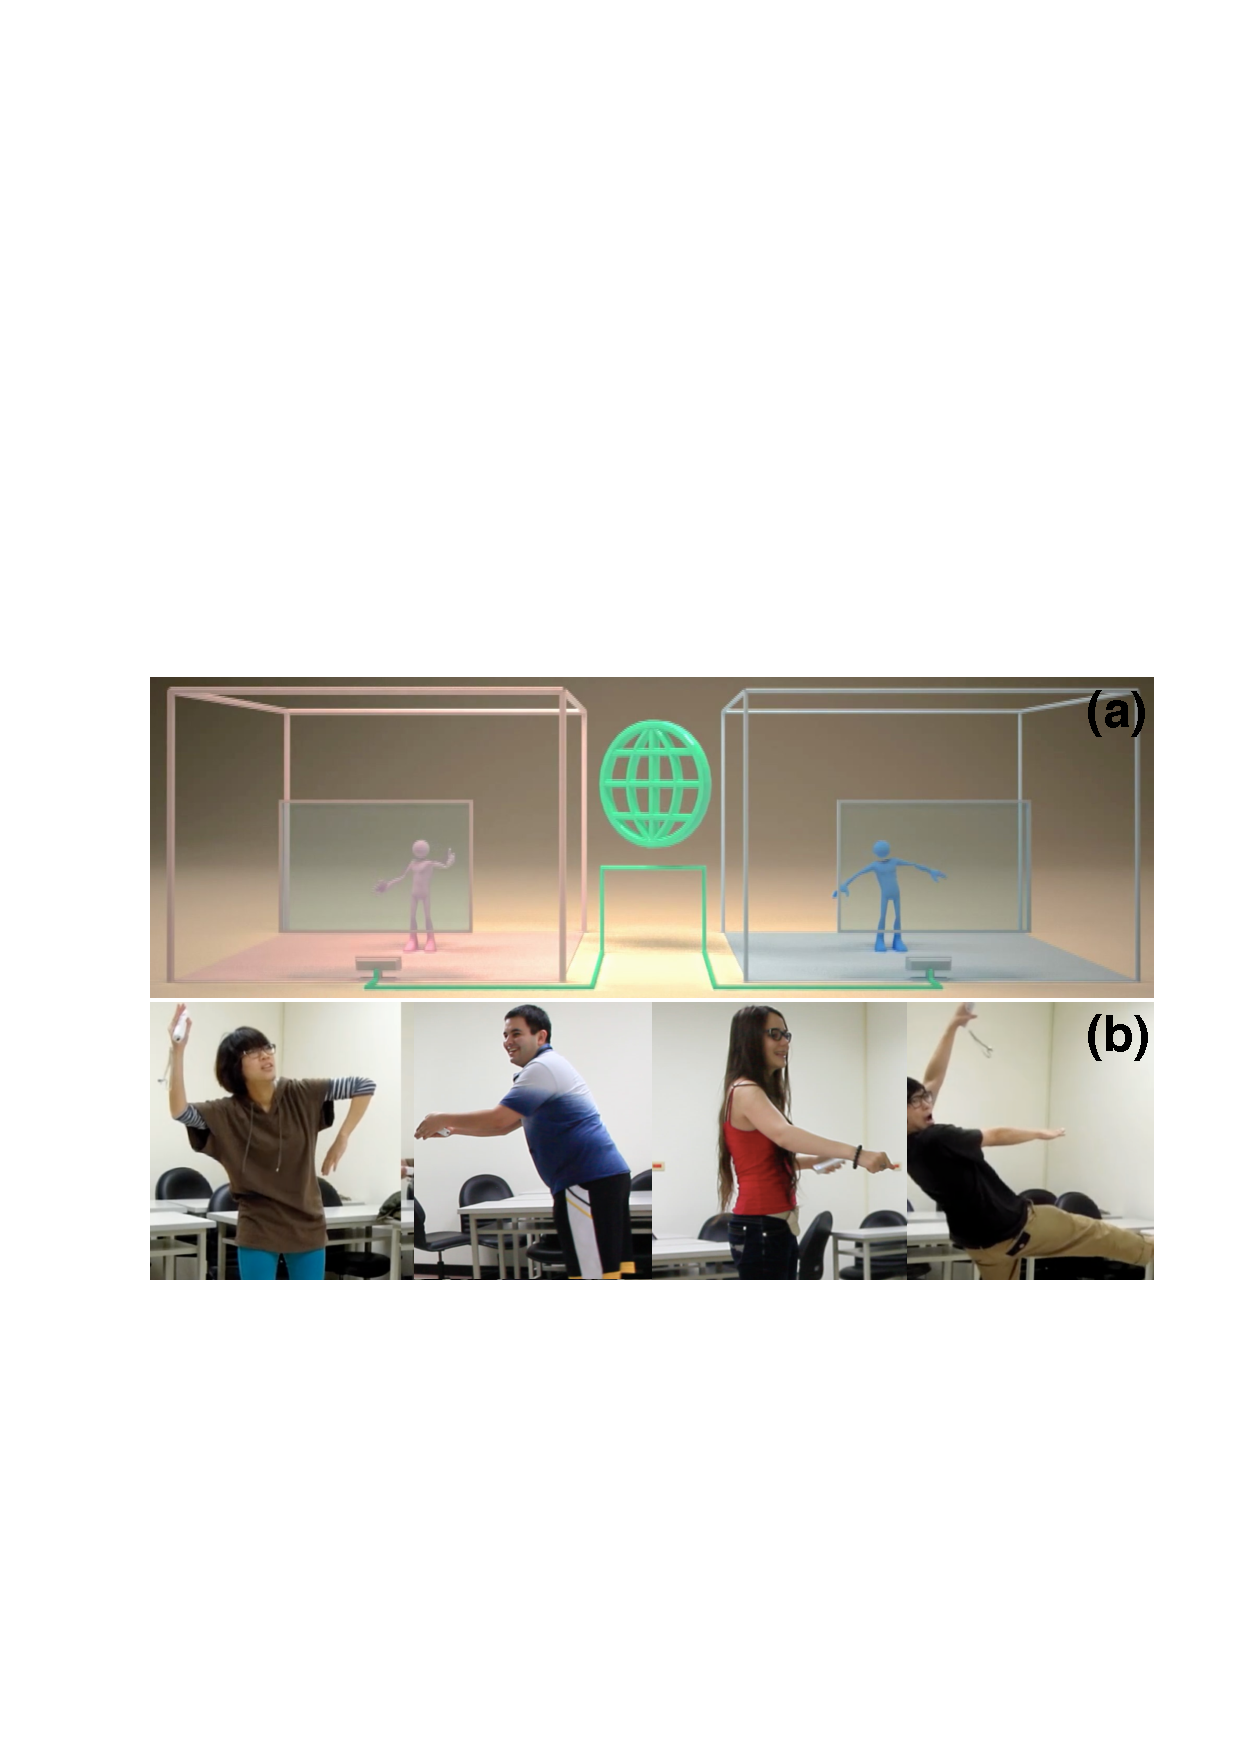
\includegraphics[width=0.9\columnwidth]{Figures/Topic.pdf}
\caption{(a) Playing cooperative games via Internet, (b) Using body language as a communication manner}
\label{fig:Topic}
\end{figure}



\section{Cooperative Game}

% Cooperative design has been an integral part of many games. With the success of games like Left4Dead,Portal 2,Gears of War, many game designers and producers are currently exploring the addition of cooperative patterns within their games.
% Cooperative Games encourage participation and collaboration, the goal is not to win as player but as a team of players. Discovering effective cooperative game patterns is an elusive and important problem.

In a growing diversity of generations, cooperative game has been an integral part of today's game development. There are a variety of great cooperative game such as Left4Dead, Portal 2, and Gears of War. With so many success cooperative game in the market, We can find out that it is a trend for game designers and related company to explore more and more cooperative patterns within their games. Cooperative games not only make players' collaboration but also result in players' higher game participation. To design a great cooperative game, the main idea is to win the game with team members rather than a single person. As we mentioned above, we know that it  is important for game designers to find out great cooperative patterns, but it also becomes a elusive problem to discover an effective cooperative game patterns.

% Some researchers analyzed a set of cooperative games to develop cooperative game design patterns. Zagal et al., for example, explored cooperative patterns within board games[1]. Also, Bjork and Holopainen presented a large number of game design patterns [2], which included cooperative and social interaction patterns.In addition Zagal et al, presented an ontology for analyzing game play [3]. Rocha et al. presented a framework of several cooperative game design patterns[4] .

In order to develop cooperative game design patterns, several researchers analyzed a set of cooperative games. For example, Zagal et al. explored cooperative patterns within board games \cite{1}, and it also presented an ontology with a view to analyzing game play \cite{3}; Bjork and Holopainen, which presented a large quantity of game design patterns \cite{2}, included cooperative and social interaction patterns; Rocha et al. presented a framework of several cooperative game design patterns \cite{4}.

% Special cases in cooperative game also become a exploring area. Wolmet et al.reports on a study of how parents and children play several cooperative co-located games with different characteristics[5]. Mark et al [6]. evaluate the communicative and cooperative behavior of same-age and mixed-age pairs (Young-Young, Young-Old, Old-Old),and identified noticeable differences between the group-types. Hamilton et al [7], explored how to design games for children with cerebral palsy to play ,and presents several cooperative gameplay prototypes.

We can realize some principle to generate cooperative game design patterns from many general cases. However, if we are eager to comprehend cooperative game design completely, some special cases in cooperative game are also an inevitable exploring area. For instance, Wolmet et al. reported a study of how parents and children play several cooperative co-located games with different characteristics \cite{5}; Mark et al. \cite{6} evaluated the communicative and cooperative behavior of same-age and mixed-age pairs (Young-Young, Young-Old, Old-Old), and identified noticable difference between group types; Hamilton et al. \cite{7} explored how to design games for children to play with cerebral palsy, and it also presented several cooperative gamplay prototypes.

% With rapid development of Internet, playing cooperative game with player from different country become a normal situation, but cooperative game for different language speaker is still an untapped area. In this work, we want to understand how language boundary affect cooperative game experience, and how to design a game that avoid negative game experience while playing with different language speaker.

With the rapid development of Internet, it is common for players to play cooperative games from different country. Nonetheless, players consist of different language speakers are still an untapped area for cooperative game design. In our work, we want to understand how language boundary affects cooperative game experience and how to design a game which can avoid negative gameplay experience while playing with different language speakers.



\section{Pilot Study}

% To understand how language boundary affect cooperative game experience, we recruit 9 Taiwaneses and 3 Japaneses and divided into 2 separate group-types(i)Taiwan-Taiwan, (ii)Taiwan-Japan. We have validated that Taiwanese players don’t understand Japanese and vise versa. We choose three different cooperative games on Steam[1] (so that player can talk to each other through Steam Talk), Rocketbirds:Hardboiled Chicken(Cooperative Action Game) ,Portal 2 (Cooperative Puzzle Game), Monaco (Cooperative Stealth Game).To emulate quick match via Internet, two players are playing these games at two distinct rooms using headphones for communication. Players play these three games 30 minutes for each. After playing each game, players will fill up an eSFQ[2] questionnaire for rapid assessment of game experiences and conduct an open-ended interviews.

In order to understand how language boundary affect cooperative game experience, we proceeded pilot study, added a factor of language boundary, for players to play the famous cooperative game on the market today. We recruited players with 9 Taiwaneses and 3 Japanese, and we divided them into 2 separated group-types: (i)Taiwan-Taiwan, (ii)Taiwan-Japan. We had confirmed that all Taiwanese players don't understand Japanese and vice versa. We choosed three different famous cooperative games: Rocketbirds:Hardboiled Chicken (Cooperative Action Game), Portal 2 (Cooperative Puzzle Game), Monaco (Cooperative Stealth Game). In addition, all three games were chosen from Steam\cite{PS1} so that players can talk to each other through Steam Talk. Besides, in order to emulate quick connection via Internet, both players were placed at two different rooms and used headphones to communicate with each other. Each time players proceed these three games for 30 minutes. Last but not least, we would like to assess game experiences and conducted an open-ended interviews, players had to fill up an eSFQ\cite{PS2} questionnaire after playing each game respectively.






\section{Game Design}

% Base on our pilot study results, we understand that if the cooperative game require High-Level Feature Communication, play it with non-common language player is really frustrating. According to GameFlow[1], games challenging should match the player’s skill level, If the challenges are greater than the skills, the result is anxiety and frustrating, if the challenges are less than the skills, the result is apathy and boring.

Based on our pilot study results(see Table 2), we realize that if playing cooperative games requires high-level-feature communication, playing with different language players would feel deeply frustrated. According to GameFlow\cite{GD1}, game challenges should match the player's skill level. If the challenges are greater than the player's skills, the gameplay result will be anxiety and frustrated. But, by constrast, if the challenges are less than the player's skills, the result will be apathy and bored.

% According to our observation, play cooperative game with different language speaker will significantly decrease cooperative skills which is really important for most cooperative games and the game challenge become too hard for this situation and causing frustrating. The most easy way to solve this problem is to decrease the game challenge difficulty for non-common language players, but it is not practical for commercial games because the players with common language would feel boring with no difficulty.

According to our observation, playing cooperative game with different language speaker will significantly decrease cooperative skills which is really important for most cooperative games. And game challenges would become too hard for this situation and cause frustrated. The easiest way to solve this problem is to decrease the game's difficulty for non-common language players. Nevertheless, this method is not practical for commercial games because it will make players with common language feel bored with no difficulty while playing the game (see Figure~\ref{fig:GD_F1}).  

\begin{figure}[!h]
\centering
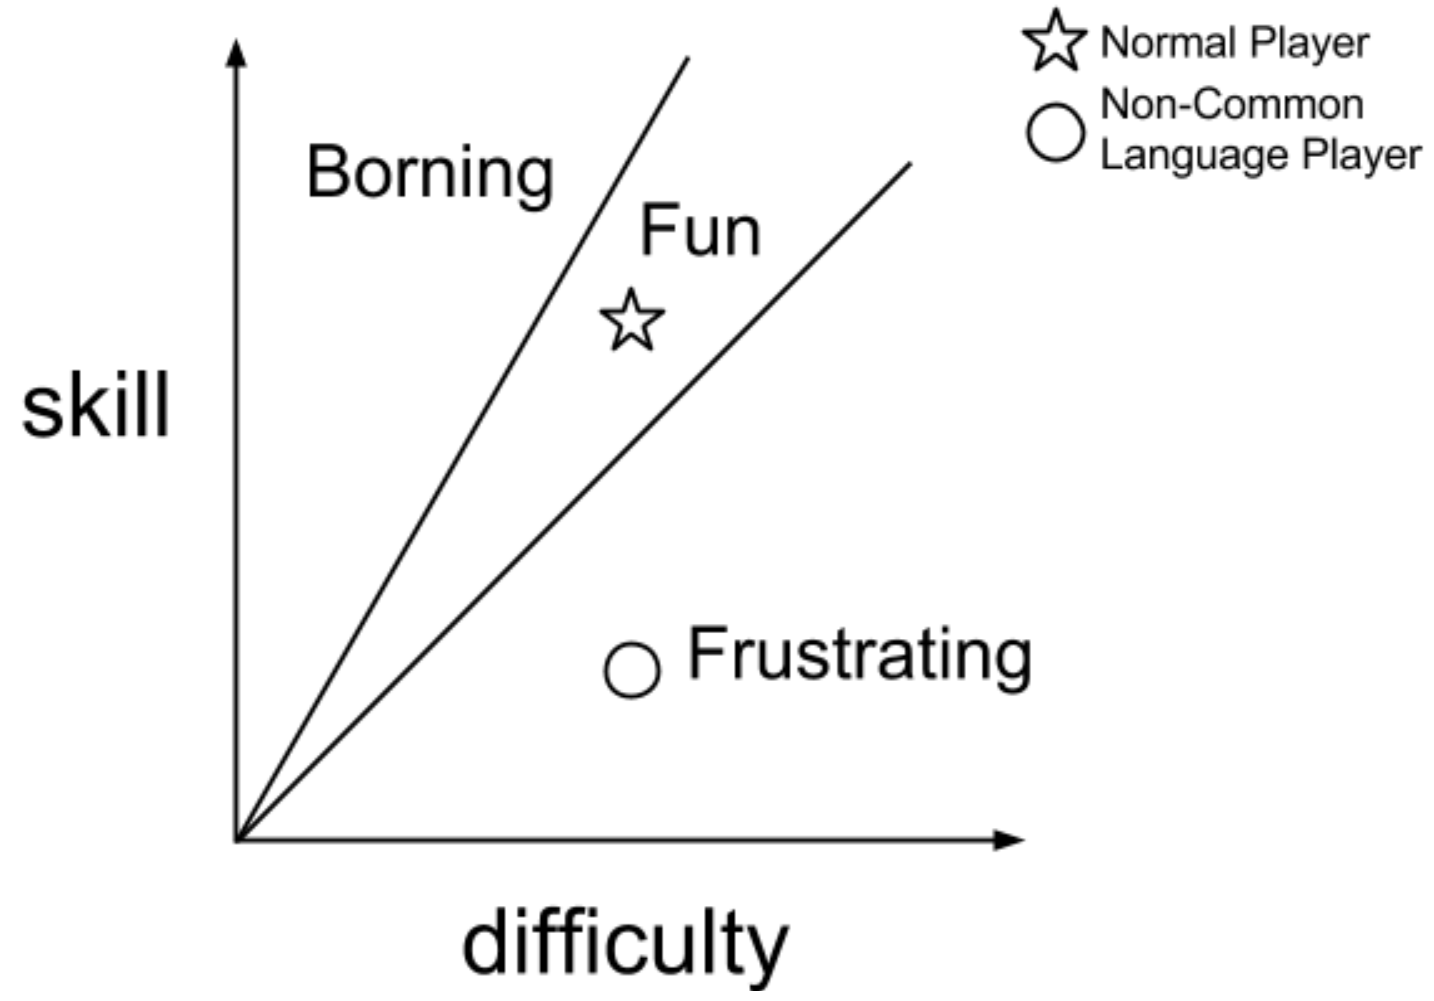
\includegraphics[width=0.9\columnwidth]{Figures/GD_F1.png}
\caption{Language boundary is causing player's skill difference}
\label{fig:GD_F1}
\end{figure}

\subsection{Body Language}

% Human communication involves not only speech, but also a wide variety of gestures and body motions. Body language is the most effective means of communicating un-spoken emotions, a non-verbal way to impart your thoughts without verbalizing it. According to The 7\% Rule [1], communication is only 7 percent verbal and 93 percent non-verbal. The non-verbal component was made up of body language(55 percent) and tone of voice (38 percent).

Consist of human communication, there are not only speech but also inclusive of various gestures and body motions. Body language, a non-verbal way to transmit your thoughts without verbalizing. Accouring to The 7\% Rule\cite{GD2}, the influence for communication for verbal is only 7\% but is 93\% for non-verbal expression. And the non-varbal expression is made up of body language (55\%) and tones of voice (38\%).

% Charades[2] is a word guessing game.In the form most played today, it is an acting game in which one player acts out a word or phrase, often by miming similar sounding words, and the other players guess the word or phrase. The idea is to use physical rather than verbal language to convey the meaning to another party.

Charades\cite{GD3} is a word guessing game. Charades is an acting game in which one player acts as a word or a phrase, and sometime imitates a similar pronounced words, while the other players guess for the answer. The main idea is to use body to make physical expression rather than using verbal language. 

% Inspired by The 7\% Rule and Charades, We suggest to use body language as a communication manner in cooperative game to normalize player’s communication skill, so that no matter players are playing with different language speaker or not, their communication skill is near enough for game developer to design a proper difficulty to please players.

Inspired by The 7\% Rule and the Charades, we suggested to use body language as a communication manner in cooperative game to normalize player's communication skill. With this idea, whether players are playing with different language speakers or not, their communication skill is near enough for game developer to design a proper difficulty to entertain players.


\subsection{Prototype - Mute Robot}

% To explore our idea that using body language communication in cooperative game , we have designed Mute Robot, a game in which 2 players must cooperate to solve a series of puzzle challenges by communicating through body language only.

The main idea we want to explore is the influence of using body language in cooperative game. In order to find out the answer, we had designed Mute Robot, a game in which 2 players must cooperate to solve a series of puzzle challenges by communicating through body language only.

To encourage players to use body language, we have designed an asymmetric puzzle system, with only one player receiving puzzle hints. The player will use body language to guide the other player to solve the puzzle. Taking one of our game stage as an example (see Figure~\ref{fig:GD_F2}), there is a locked door on the right side which obstructs both players’ route to the next stage. The top player can’t see the puzzle-solving hints but can turn the wheel to the match the puzzle answer, which consequently opens the locked door. The only way to pass the stage is for the bottom player to convey the puzzle-solving messages to the other player with body language.

\begin{figure}[!h]
\centering
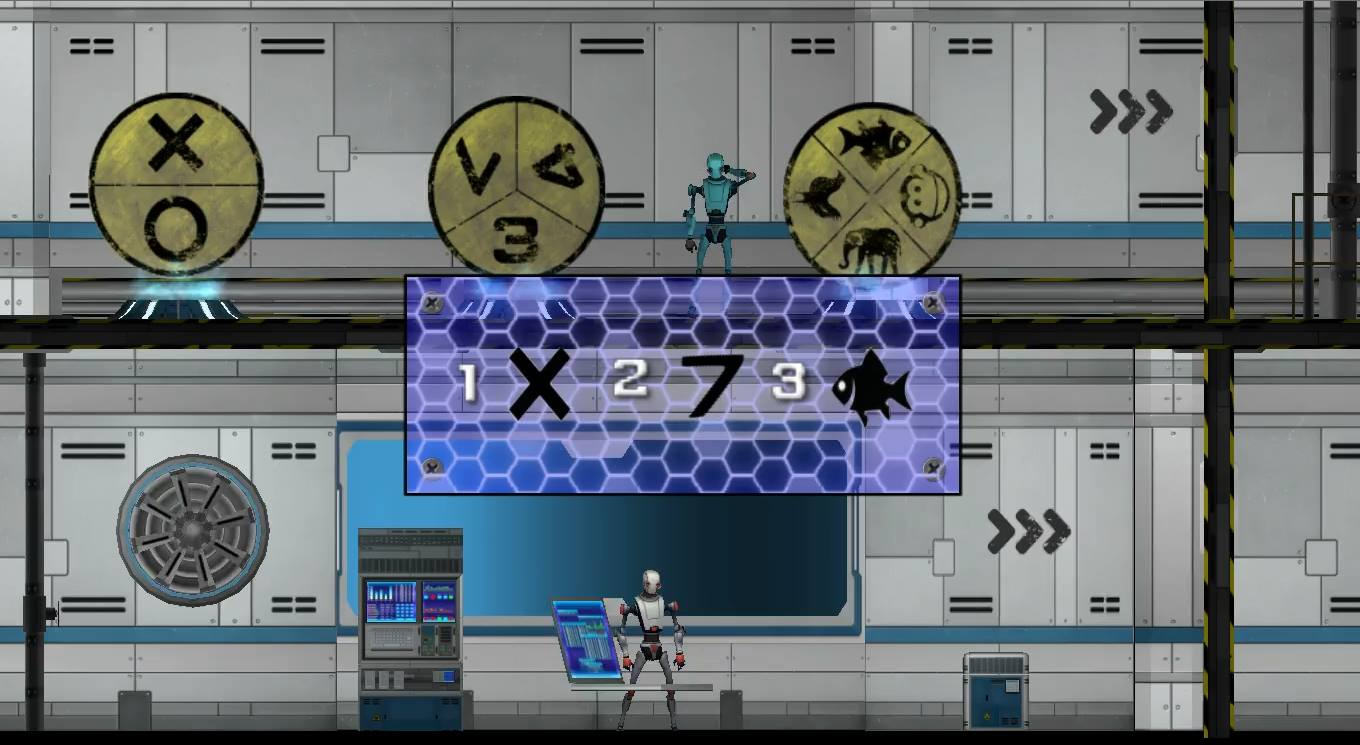
\includegraphics[width=0.9\columnwidth]{Figures/GD_F2.jpg}
\caption{The asymmetric puzzle game design in one of Mute Robot’s stages.}
\label{fig:GD_F2}
\end{figure}


\subsection{Level Design}

% To test the limitation of body language in cooperative game, we designed three puzzles with incremental difficulty. Every message for player to transmit is getting more and more complex.

In order to test the limitation of using body language in cooperative game, we designed three puzzles with incremental difficulty, which means that the message player needed to transmit will have higher complexity than previous one. Next we introduce each game level respectively.

% In the first level, we are testing sequence message to transmit which is a classic cooperative game puzzle. One player has to express the secret sequence to another player, so that he can press the apparatus buttons in correct sequence, then open the door and route to next puzzle.

In the first level, we test sequence messages whether to be transmitted or not. This is a classic puzzle in cooperative game. One player has to express the secret sequence to another player so that another player can press the apparatus buttons in correct order. If the order is correct, the door will open and both players can proceed to the next level.

% In the second level, there are three apparatus wheel to turn to the correct pattern. The symbols on the first wheel are two state of boolean value (circle and cross), and the second wheel’s symbols are numbers (3,4,7), the symbols on the last wheel are animals(fish, chicken, monkey and elephant).

In the second level, there are three apparatus wheels which need to be turned to match the correct pattern. Symbols on the first wheel are boolean value (circle and cross). The second wheel's symbols are numbers (3, 4, 7), and the last wheel's symbols are animals (fish, chicken, monkey and elephant).

% In the last level, we want to test more complex concept like emotion, so we randomly give an emotion word for player to transmit (angry, happy or tired) ,and the player on the other side needs to guess the emotion and spell it correctly.

In the last level, we want to test the concept with higher complexity, such as emtion. So we randomly provide an emotion word (angry, happy or tired) for one player and he needs to transmit to another player. The level can be passed only if another player guess the emotion and spell it correctly.

\subsection{System Implementation}

% Mute Robot is a cooperative puzzle platformer game built using Unity3D[4] engine. The game involves two players at two distinct locations connected over the Internet. The players cannot talk to each other directly and the only way to communicate is using their body language. we use Kinect to capture player’s body language and apply to their avatar. To avoid arm fatigue of mid-air interactions [1] with Kinect, each player uses a Wii[3] controller to complete trivial manipulation (e.g.move left,move right, jump, confirm, cancel). 

Mute Robot is a cooperative puzzle platformer game built using Unity3D\cite{GD4} engine. The game involves two players at two distinct locations connected over the Internet. The players cannot talk to each other directly and the only way to communicate is using their body language. We use Kinect to capture player's body language and apply to their avatar. In order to avoid arm fatigue of mid-air interactions\cite{GD6} with Kinect, each player uses a Wii\cite{GD5} controller to complete trivial manipulation (e.g. move left, move right, confirm, cancel).




\section{User Study}

Our goal is to explore how body language affects cooperative experience for players with and without common languages. 

\subsection{Study Design and Participants}
We set up our prototype game with three distinct communication modes: speaking only, body language only, and both speaking and body language. 

%To compare our solution with traditional setting, we provided three different types of communication manners to play Mute Robot. We divided users into two groups by whether they have the same native language or not. So there are common language and different language groups respectively. Different language group are required to use their native language to communicate with each other. About our experiment, every team will have two players and be placed in two distinct rooms. Players play Mute Robot with each other through the Internet connection. Totally we tested 24 groups with 48 users (34 male and 14 female, average age is 22.6), inclusive of 12 common language groups and 12 different language groups (36 Taiwanese, 5 Japanese, 2 German, 1 Netherlander, 1 Chilan, 1 Iraqi, 1 Russian, 1 Guatemalan).
%
%\subsection{Method}
%
%In our experiment, we provided three different types of communication manners to play Mute Robot:
%\begin{enumerate}
%    \item Speaking: 
%    traditional gameplay manner, user can communicate through speaking language.
%    \item Body Language: 
%    players can communicate through body language only.
%    \item Both:
%    players can communicate with each other through speaking language and body language.
%\end{enumerate}

Each pair of players were placed into two separate rooms, so that they could not see nor hear each other. The rooms were on the same local area network to minimize network latency. At the beginning of each session, players practiced controlling the avatars via Kinect and Wii controllers and speaking to their partners through voice over IP (VOIP). 

Each pair of players completed all Mute Robot stages three times, each time using one of three communication modes. The order of the communication modes was counterbalanced to eliminate the effects of ordering.
Each time the players completed Mute Robot using one of the communication modes, they filled out a Short Feedback Questionnaire (eSFQ)\cite{eSFQ} questionnaire to rate their experience. 

At the end of the session, the players filled out a final questionnaire comparing their preferences, and we conducted interviews to get their qualitative feedback. Each session took about 1 hour to finish. 
In addition, all the gameplay was recorded on video and we manually coded them using Cooperative Performance Metrics (CPM)\cite{CPMs}. 

We recruited 48 participants (15 females) with average age of 22.6, for a total of 24 pairs of participants. Half of the participant pairs shared a common language (Mandarin). The other half of the pairs were ask to speak in a language that could not be understood by their partners (12 Taiwanese speakers paired with 5 Japanese, 2 German, 1 Netherlander, 1 Chilean, 1 Iraqi, 1 Russian, and 1 Guatemalan).
  
% After our user study, we used eSFQ, CPMs, and a final questionnaire to evaluate the Mute Robot gameplay experience between different communication manners.

%conduct video recording at all experiment process and used these video to do CPMs\cite{CPMs} (see Figure~\ref{fig:US1}), 

% \begin{figure}[!h]
% \centering
% 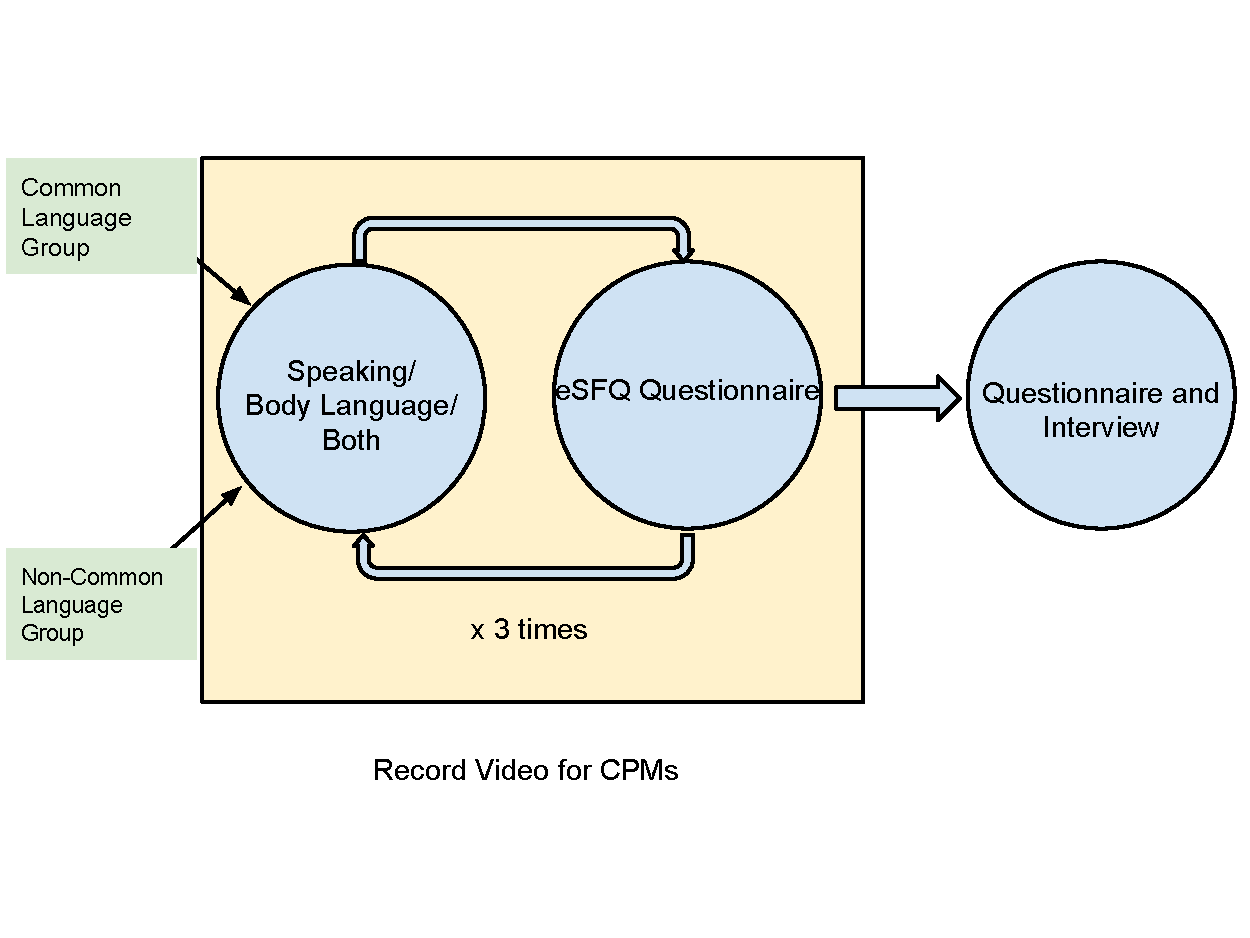
\includegraphics[width=0.9\columnwidth]{Figures/US_F1.pdf}
% \caption{User study flow}
% \label{fig:US1}
% \end{figure}

% \subsection{Result}

%After our user study, we used eSFQ, CPMs, and a final questionnaire to evaluate the Mute Robot gameplay experience between different communication manners.




\subsection{Short Feedback Questionnaire (eSFQ) Results}
In our analysis, we focus on the fun/enjoyment ratings and both the positive and negative co-experience as described through the selected keywords. 

% eSFQ\cite{eSFQ} had been proved that it is a questionnaire for rapid assessment of game experience. eSFQ capture the experienced fun/enjoyment, curiosity, and co-experience. 

% We used five-point likert scale ranging from ``I completely agree'', ``I agree'', ``neither/nor'', ``I disagree'' to ``I completely disagree''.

\subsubsection{Fun/Enjoyment Ratings}

% \begin{figure}[!h]
% \centering
% 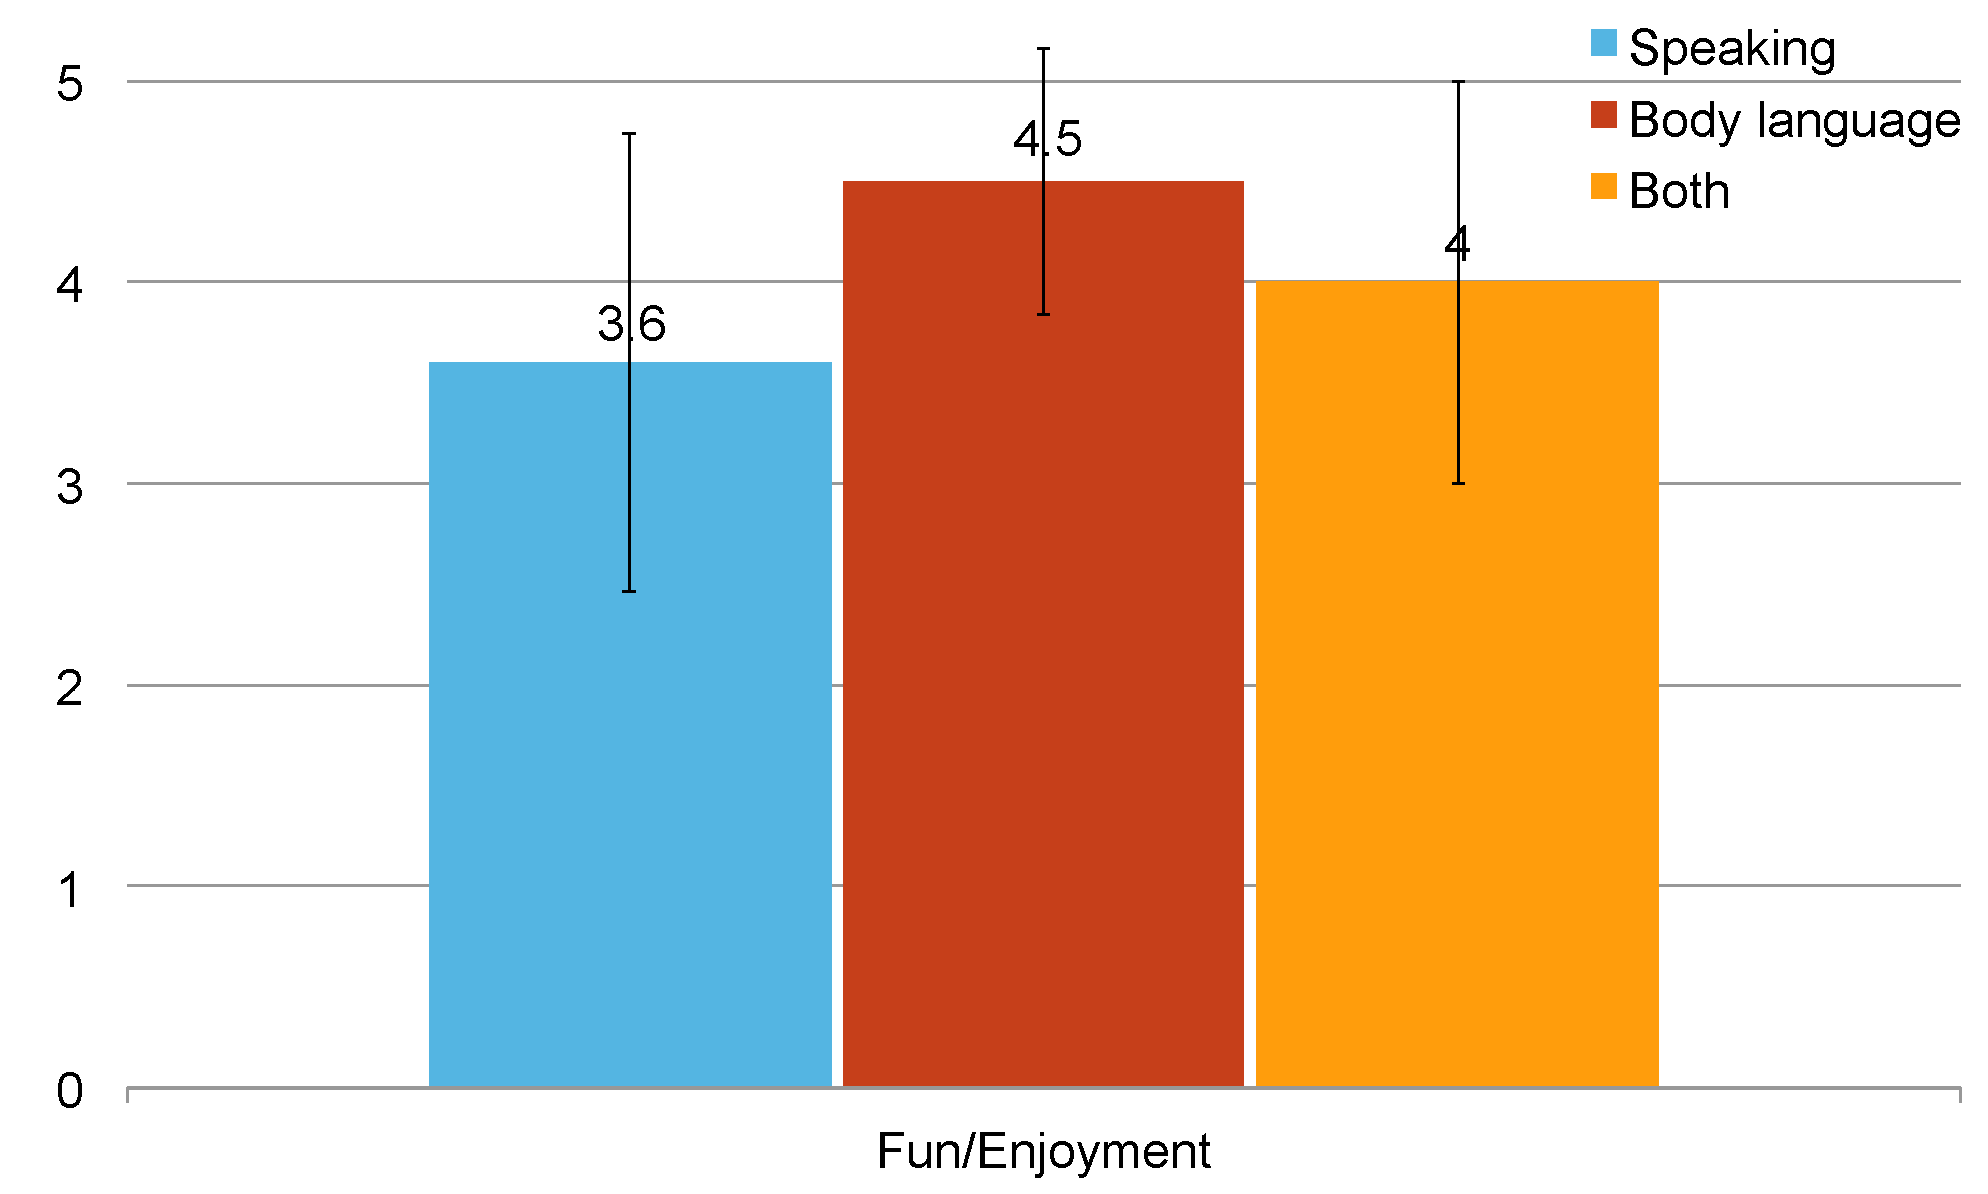
\includegraphics[width=0.9\columnwidth]{Figures/US_Fun_Com.pdf}
% \caption{eSFQ: fun/enjoyment index for Common Language Group.}
% \label{fig:US_Fun_Com}
% \end{figure}

% \begin{figure}[!h]
% \centering
% 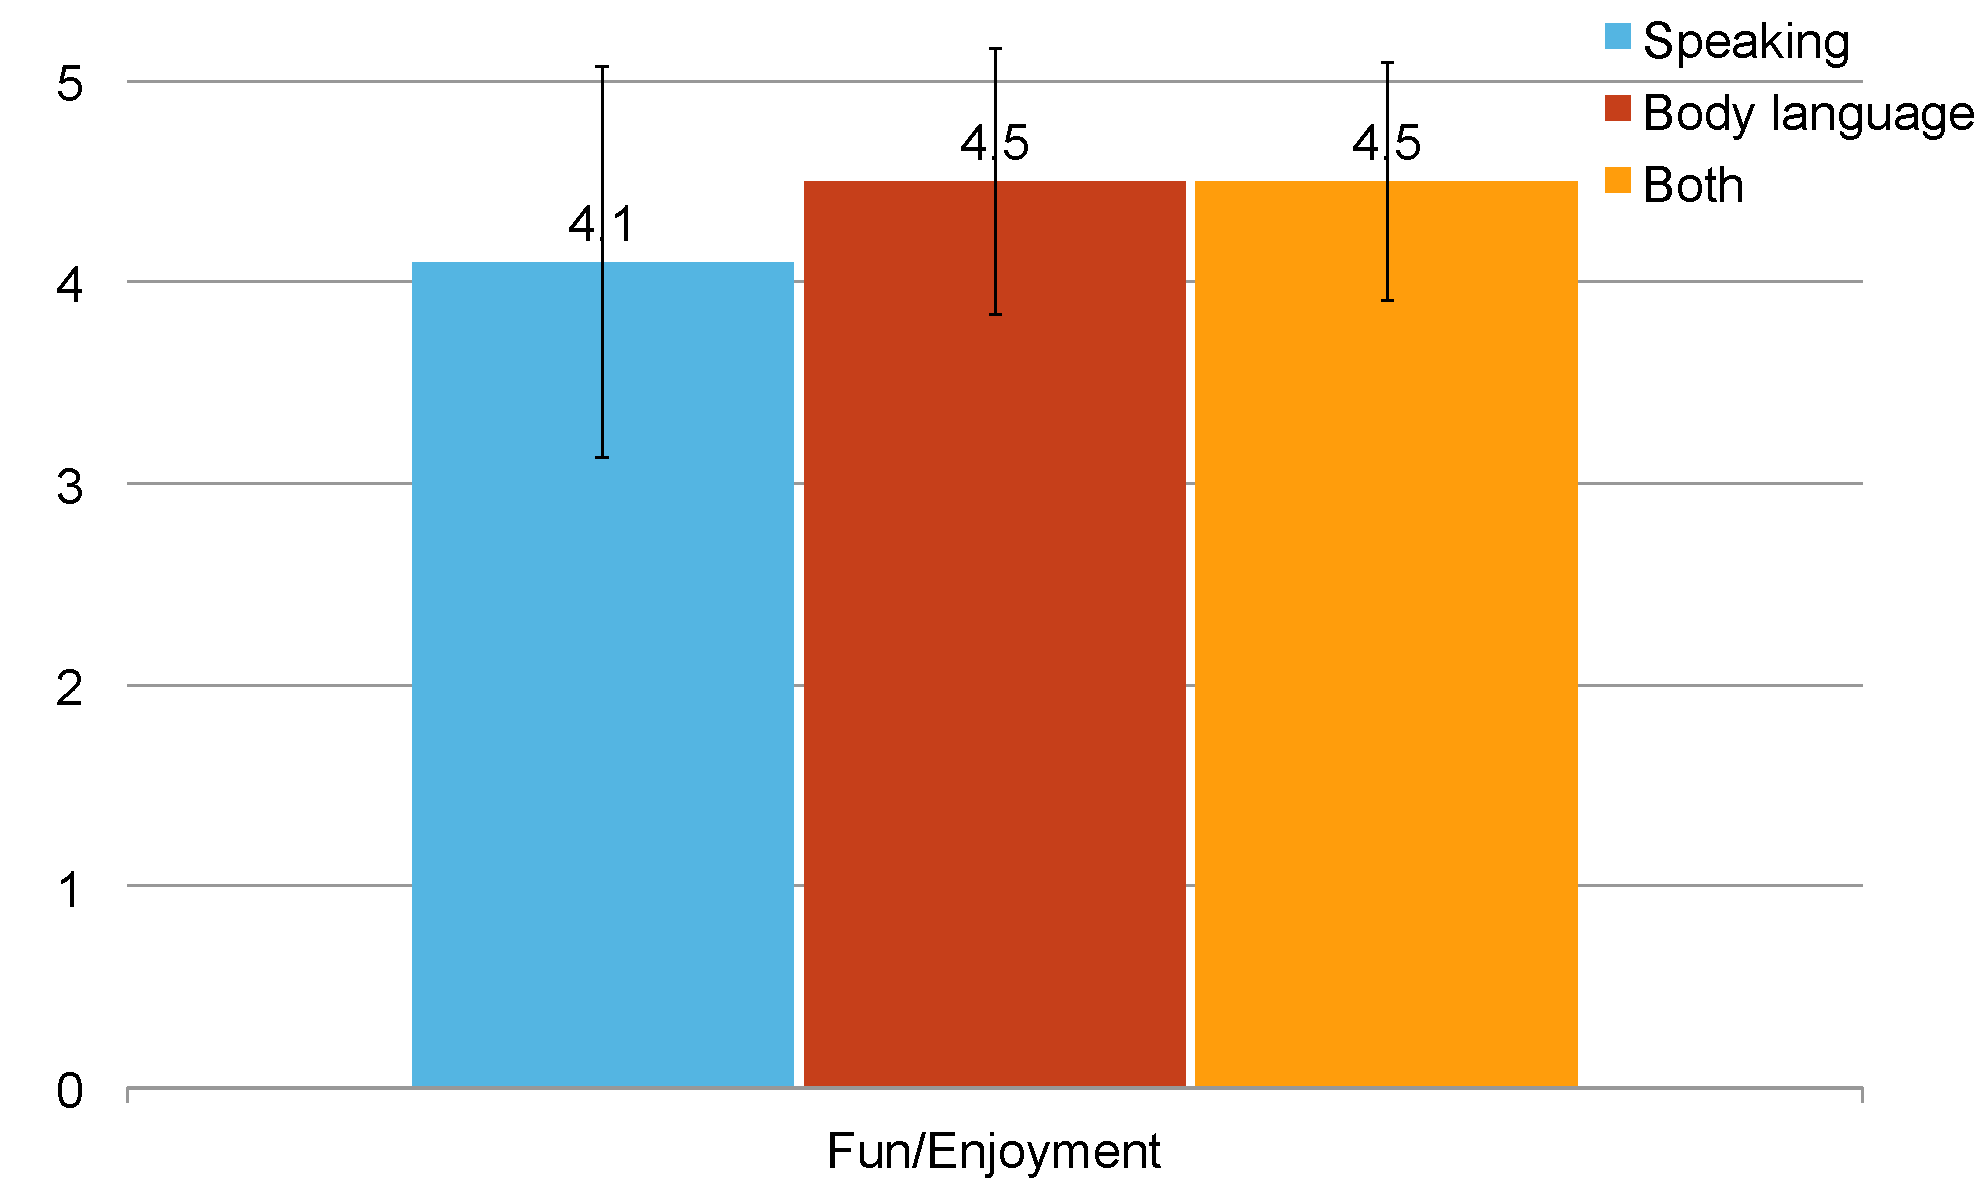
\includegraphics[width=0.9\columnwidth]{Figures/US_Fun_Dif.pdf}
% \caption{eSFQ: fun/enjoyment index for Different Language Group.}
% \label{fig:US_Fun_Dif}
% \end{figure}

\begin{figure}[!b]
\centering
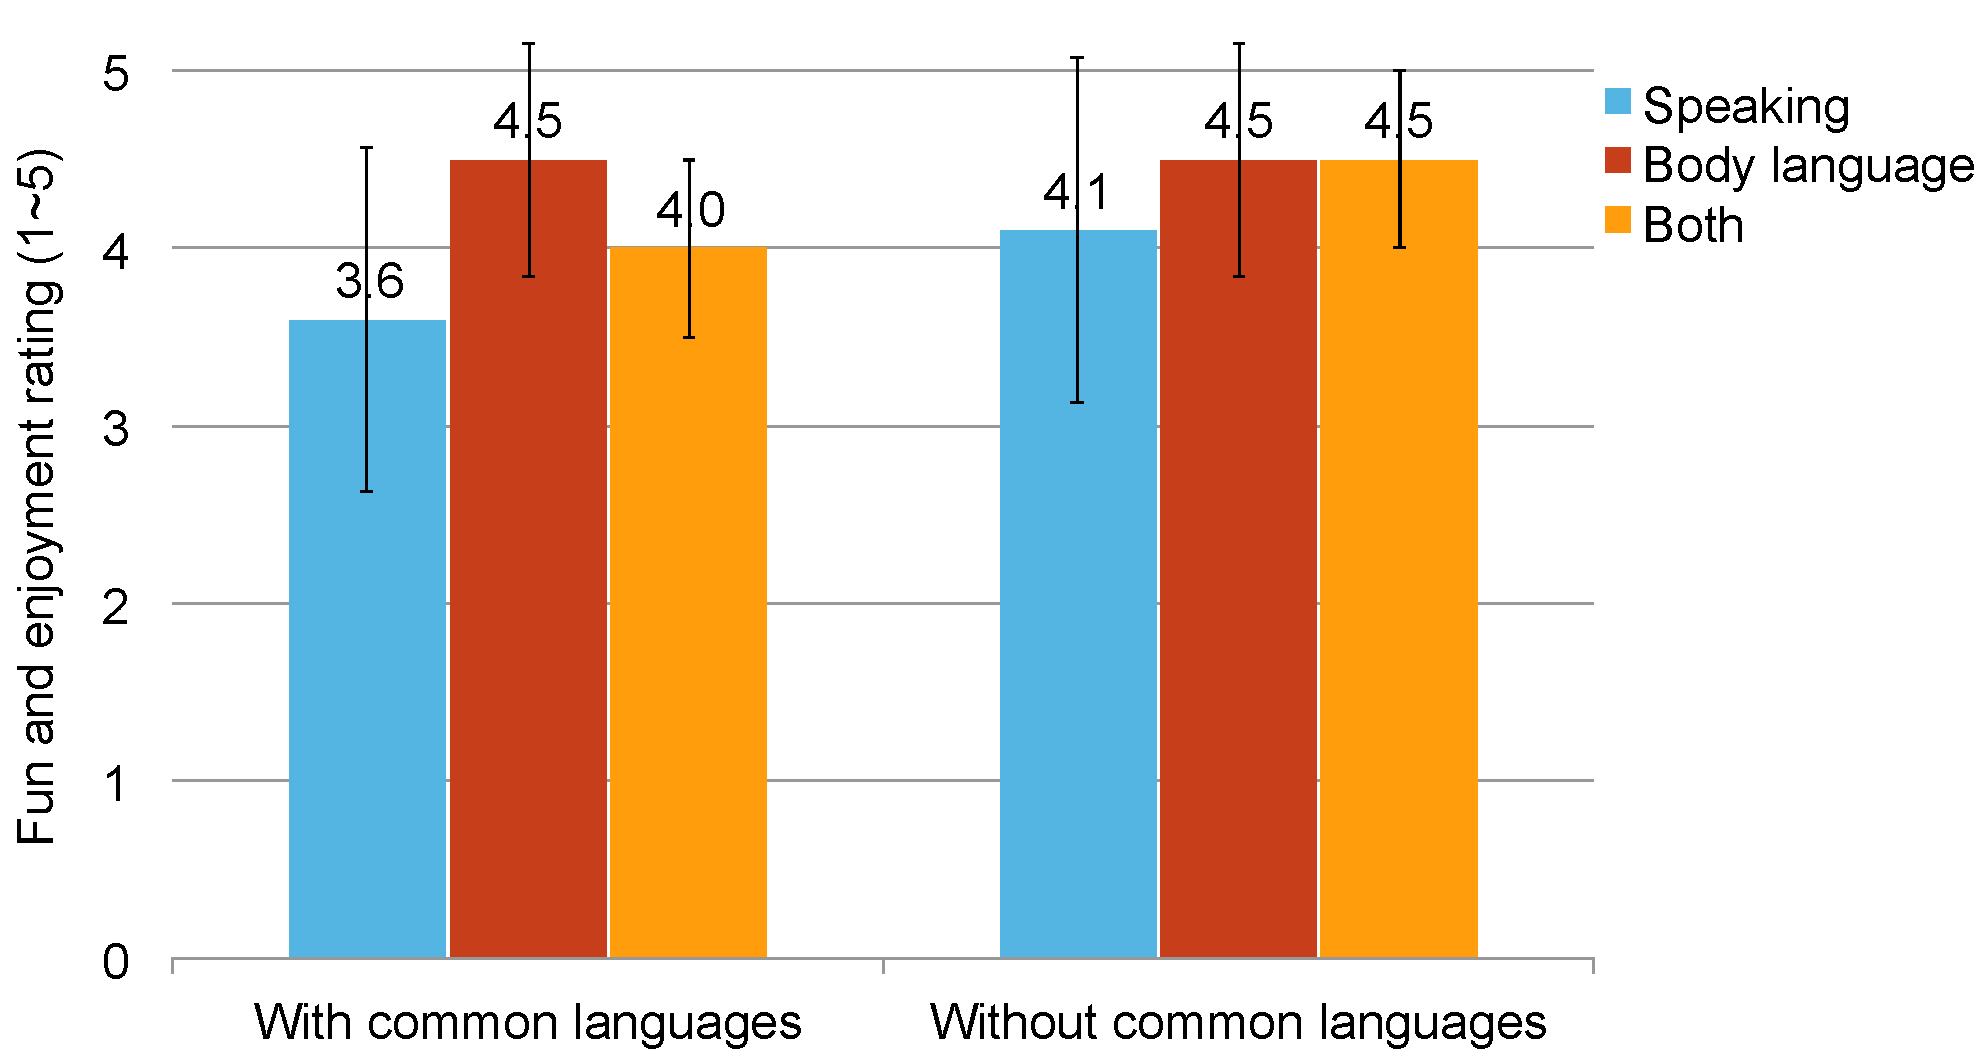
\includegraphics[width=0.9\columnwidth]{Figures/US_Fun.pdf}
\caption{eSFQ: fun/enjoyment rating for players \textit{with} and \textit{without} common languages.}
\label{fig:US_Fun}
\end{figure}


% \begin{figure}[!h]
% \centering
% 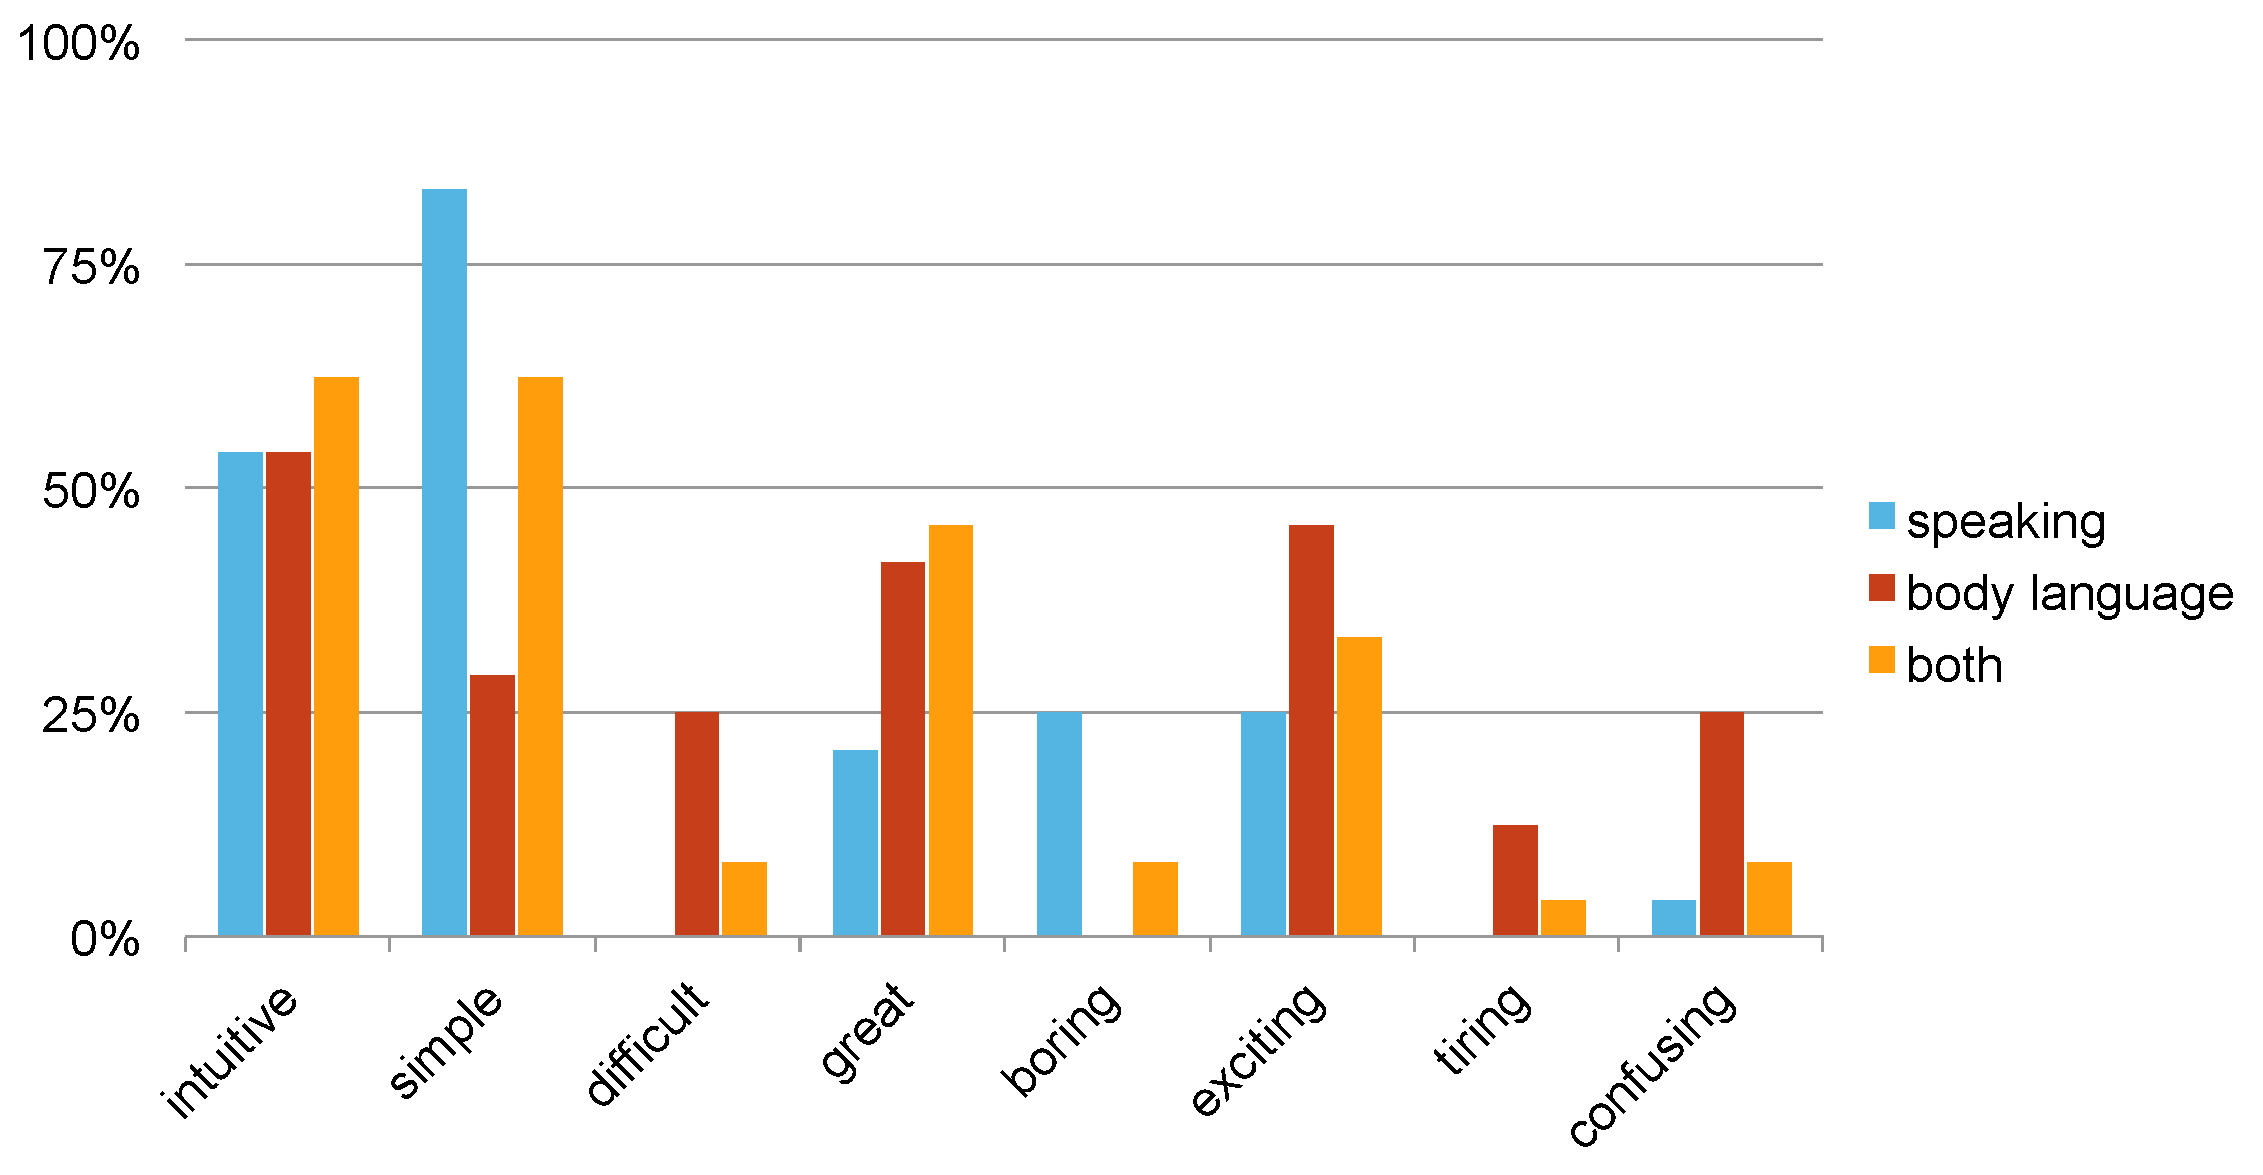
\includegraphics[width=0.9\columnwidth]{Figures/US_eSFQ_Com_Fun.pdf}
% \caption{eSFQ: fun/enjoyment game experience analysis for common language group.}
% \label{fig:US_eSFQ_Com_Fun}
% \end{figure}

% \begin{figure}[!h]
% \centering
% 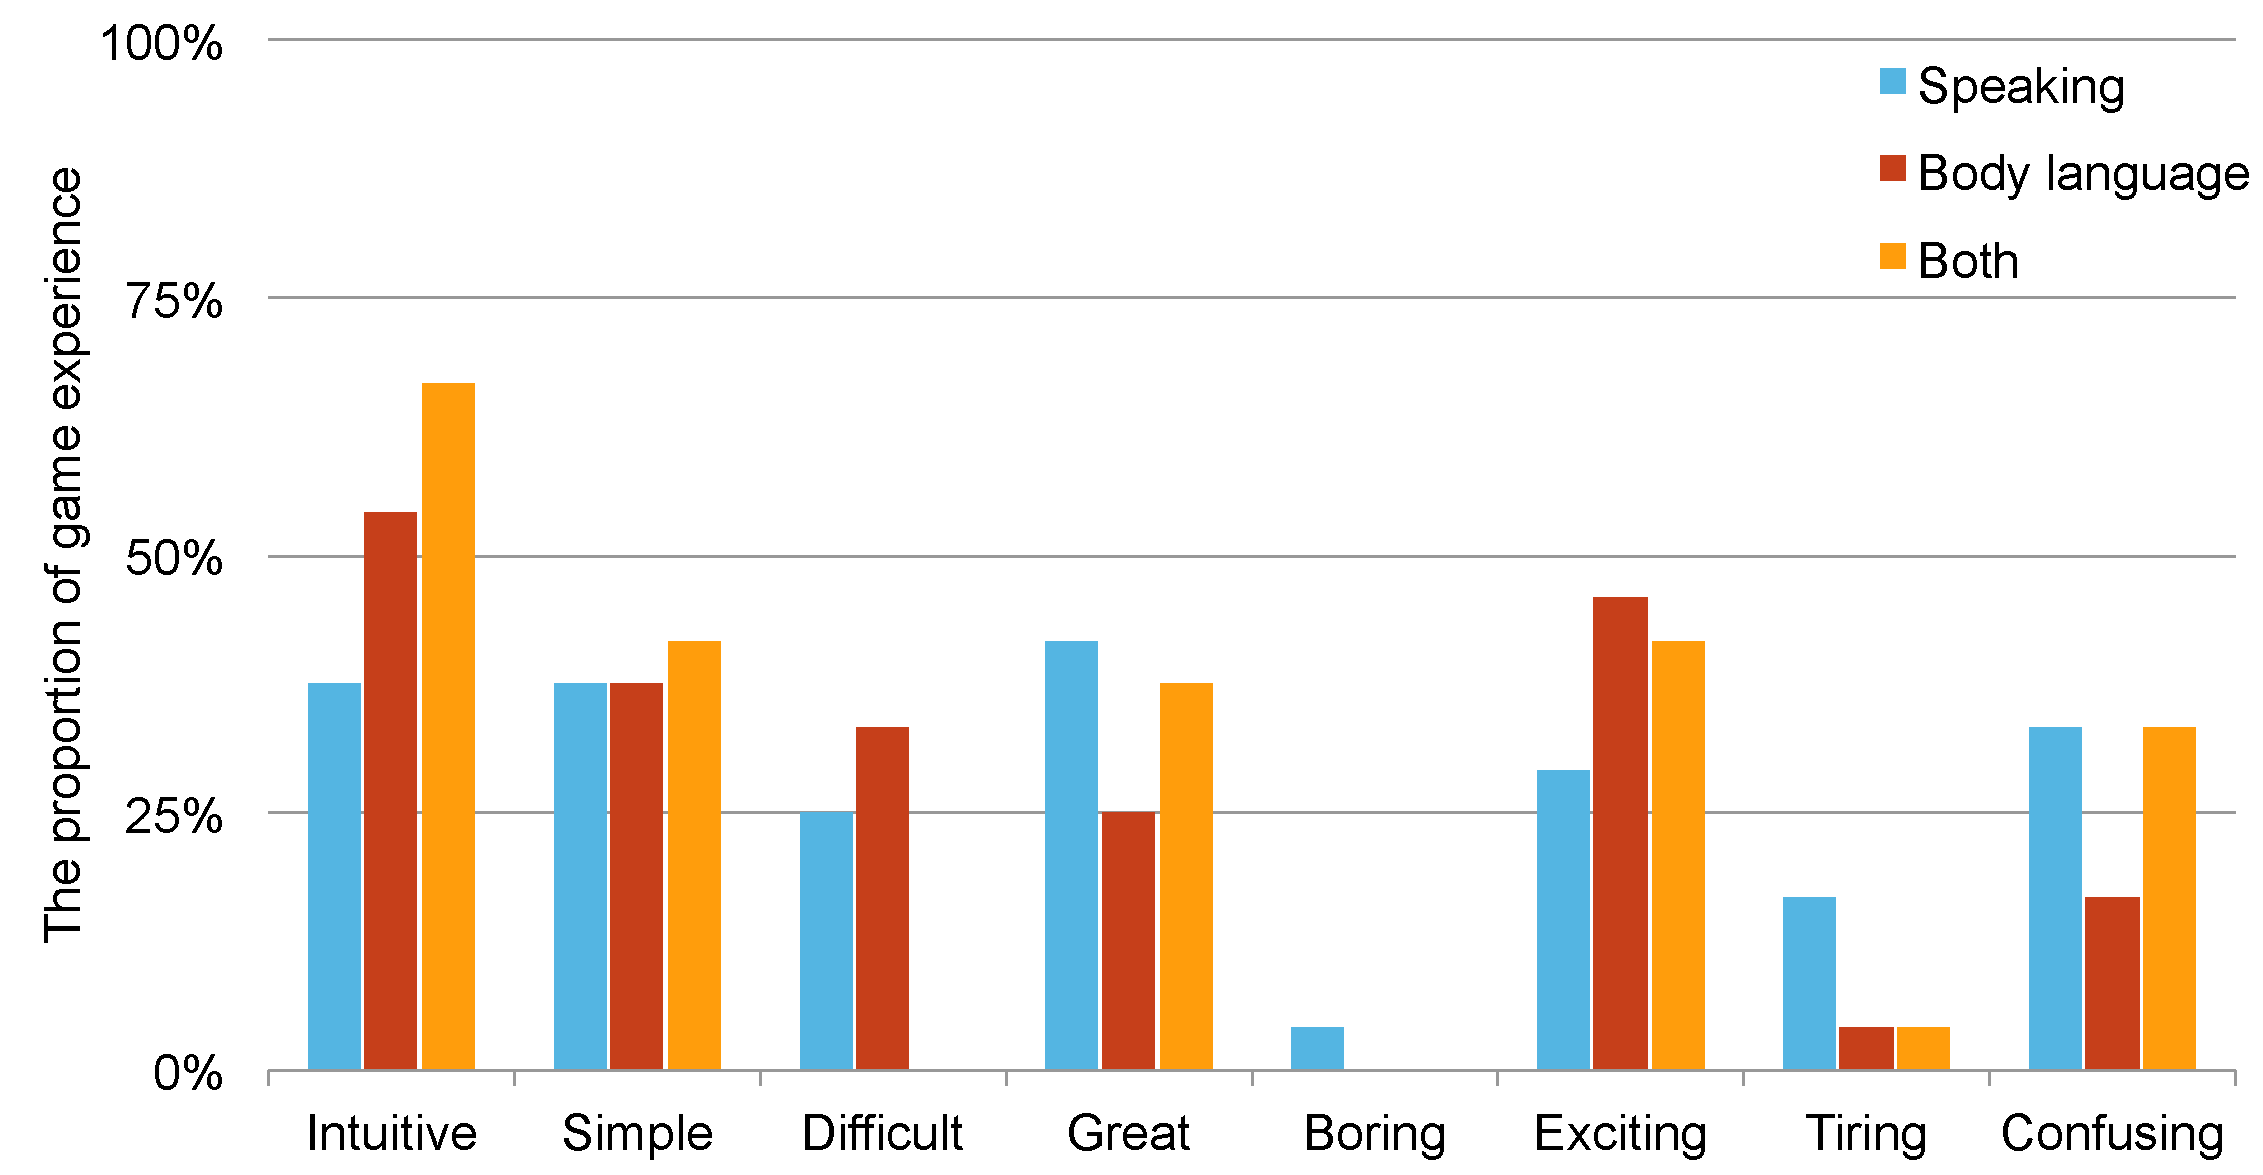
\includegraphics[width=0.9\columnwidth]{Figures/US_eSFQ_Dif_Fun.pdf}
% \caption{eSFQ: fun/enjoyment game experience analysis for different language group.}
% \label{fig:US_eSFQ_Dif_Fun}
% \end{figure}

%and ~\ref{fig:US_eSFQ_Com_Fun}

% For common language group (see Figure~\ref{fig:US_Fun_Com}), the mean of the experienced fun level for ``Speaking'' was 3.58 (SD = 1.14) (5 meaning ``Yeah, fun'' - highest level of fun and 1 meaning ``Yawn, boring'' - lowest level of fun). Their game experiences were related to simple (83\% of the users), and intuitive(54\%). The mean of the experienced fun level for ``Body language'' was 4.54 (SD = 0.66). Their game experiences were related to intuitive (54\%), exciting (46\%) and great (42\%). The mean of the experienced fun level for ``Both'' was 3.96 (SD = 1.00). Their game experiences were related to intuitive (63\%), simple (63\%) and exciting (33\%). 

% For different language group (see Figure~\ref{fig:US_Fun_Dif}), the mean of the experienced fun level for ``Speaking'' was 4.08 (SD = 0.97). Their game experiences were related to great (42\% of the users), intuitive (38\%), simple (38\%), and confusing (33\%). The mean of the experienced fun level for ``Body language'' was 4.46 (SD = 0.66). Their game experiences were related to intuitive (54\%), exciting (46\%), simple (38\%) and difficult (33\%). The mean of the experienced fun level for ``Both'' was 4.50 (SD = 0.59). Their game experiences were related to intuitive (67\%), exciting (42\%), simple (42\%), great (34\%) and confusing (33\%).

Figure~\ref{fig:US_Fun} shows the fun/enjoyment rating for players with and without common languages using the three communication modes. 
For players with common languages, their mean rating for Speaking mode was 3.58 (SD = 1.14), and the most popular keywords selected were ``simple'' (83\% of the users) and ``intuitive'' (54\%). 
Their mean rating for Body language mode was 4.54 (SD = 0.66), and the most popular keywords selected were ``intuitive'' (54\%), ``exciting'' (46\%) and ``great'' (42\%). 
Their mean rating for Both mode was 3.96 (SD = 1.00), and the most popular keywords selected were ``intuitive'' (63\%), ``simple'' (63\%) and ``exciting'' (33\%). 

For players without common languages (see Figure~\ref{fig:US_Fun}), 
their mean rating for Speaking mode was 4.08 (SD = 0.97), and the most popular keywords selected were ``great'' (42\% of the users), ``intuitive'' (38\%), ``simple'' (38\%), and ``confusing'' (33\%). 
Their mean rating for Body language mode was 4.46 (SD = 0.66), and the most popular keywords selected were ``intuitive'' (54\%), ``exciting'' (46\%), ``simple'' (38\%) and ``difficult'' (33\%). 
Their mean rating for Both mode was 4.50 (SD = 0.59). , and the most popular keywords selected were ``intuitive'' (67\%), ``exciting'' (42\%), ``simple'' (42\%), ``great'' (34\%) and ``confusing'' (33\%).

% The mean of the experienced fun level for ``Body language'' was 4.54 (SD = 0.66). Their game experiences were related to intuitive (54\%), exciting (46\%) and great (42\%). 
% The mean of the experienced fun level for ``Both'' was 3.96 (SD = 1.00). Their game experiences were related to intuitive (63\%), simple (63\%) and exciting (33\%). 

% For different language group (see Figure~\ref{fig:US_Fun}), 
% the mean of the experienced fun level for ``Speaking'' was 4.08 (SD = 0.97). Their game experiences were related to great (42\% of the users), intuitive (38\%), simple (38\%), and confusing (33\%). 
% The mean of the experienced fun level for ``Body language'' was 4.46 (SD = 0.66). Their game experiences were related to intuitive (54\%), exciting (46\%), simple (38\%) and difficult (33\%). 
% The mean of the experienced fun level for ``Both'' was 4.50 (SD = 0.59). Their game experiences were related to intuitive (67\%), exciting (42\%), simple (42\%), great (34\%) and confusing (33\%).
% The fun/enjoyment rate of ``Body language'' and ``using speaking and body language together'' were better than ``Speaking'', no matter in common language group or in different language group. In sum, ``Body language'' got the best rate of fun level, and the rate of ``using speaking and body language together'' was only slightly lower than ``Body language'' but is still very good. And ``Speaking'' got the worst rate. We dicovered that the difficulty of the game would make an influence on fun. In other words, both index were in direct proportion. For instance, when the ratio of simple becomes higher, the ratio of fun will be lower than before. In addition, different language group had higher experienced fun level for ``Speaking'', but it also make users feeling confused for ``Speaking'' and``using speaking and body language together''.

% As we can see in Figure~\ref{fig:US_Fun_Com} and \ref{fig:US_Fun_Dif}, whether players have common language or not, body language has higher rate of fun/enjoyment than traditional manner(speaking). In other words, body language can enhance fun and enjoyment. According to Figure~\ref{fig:US_eSFQ_Com_Fun} and \ref{fig:US_eSFQ_Dif_Fun}, the confusing index was in contrast to common language group and different langauge group. Common language group felt that using body language was the most confused. However, different language group thought using body languagae was the least confused manner to communicate.

% As we can see in Figure~\ref{fig:US_Fun_Com} and \ref{fig:US_Fun_Dif}, whether players have a common language or not, body language has a higher rate of fun/enjoyment than traditional manner(speaking). In other words, body language can enhance fun and enjoyment.

As we can see in Figure~\ref{fig:US_Fun}, the two communication modes with body language had higher fun/enjoyment ratings compared to the speaking-only mode for all players (both with and without common languages). 

% \paragraph{2. curiosity}

% For common language group, the curiosity about ``Speaking'' was rated with a mean of 4.01 (SD = 0.85 (5 meaning very curious and 1 meaning not curious at all). ``Body language'' with 4.39 on average (SD = 0.74) and ``Both'' with 4.25 on average (SD = 0.73).

% For different language group, the curiosity about ``Speaking'' was rated with a mean of 4.04 (SD = 0.90). ``Body language'' with 4.11 on average (SD = 0.93) and ``Both'' with 4.07 on average (SD = 0.89).

% According to the curiousity index, we could find out that users were curious about the game. Analyzed data in detail, we find out that ``Body language'' had the highest rate. Second is ``Both'', and ``Speaking'' has the worst rate. But there was no significant difference between the ratings. As a result, no matter in common language groups or different language groups, communication manners has no significant impact on the index of curiosity.

% \begin{table}[!h]
% \renewcommand\arraystretch{1.5}
%   \centering
%   \begin{tabular}{
%   !{\vrule width2pt}c
%   !{\vrule width2pt}c
%   !{\vrule width2pt}c
%   !{\vrule width2pt}c
%   !{\vrule width2pt}}
%     \Xhline{2pt}
%     \multicolumn{1}
%     {!{\vrule width2pt}c!{\vrule width2pt}}
%     {\tabhead{}} &
%     \multicolumn{1}
%     {c!{\vrule width2pt}}
%     {\centering\tabhead{Speaking}} &
%     \multicolumn{1}
%     {c!{\vrule width2pt}}
%     {\centering\tabhead{Body Language}} &
%     \multicolumn{1}
%     {c!{\vrule width2pt}}
%     {\centering\tabhead{Both}} \\
%     \Xhline{2pt}
%     Common Language & 4.01 & 4.39 & 4.25 \\
%     \Xhline{2pt}
%     Different Language & 4.04 & 4.11 & 4.07 \\
%     \Xhline{2pt}
%   \end{tabular}
%   \caption{Curiosity index of eSFQ}
%   \label{tab:KappaValue}
% \end{table}


% we found out that in common language group, although the game is the same, curiosity still be impacted by communication manners. But different langauge group didn't have obvious difference.

% \begin{figure}[!h]
% \centering
% 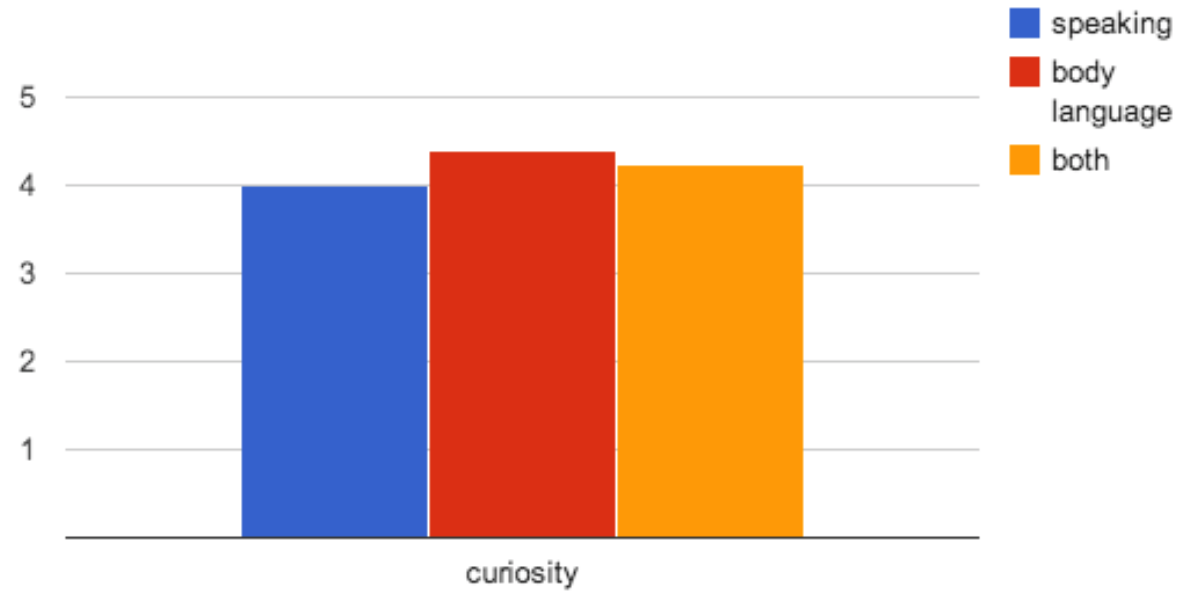
\includegraphics[width=0.9\columnwidth]{Figures/US_Curi_Com.png}
% \caption{Common Language Group}
% \label{fig:US_Curi_Com}
% \end{figure}

% \begin{figure}[!h]
% \centering
% 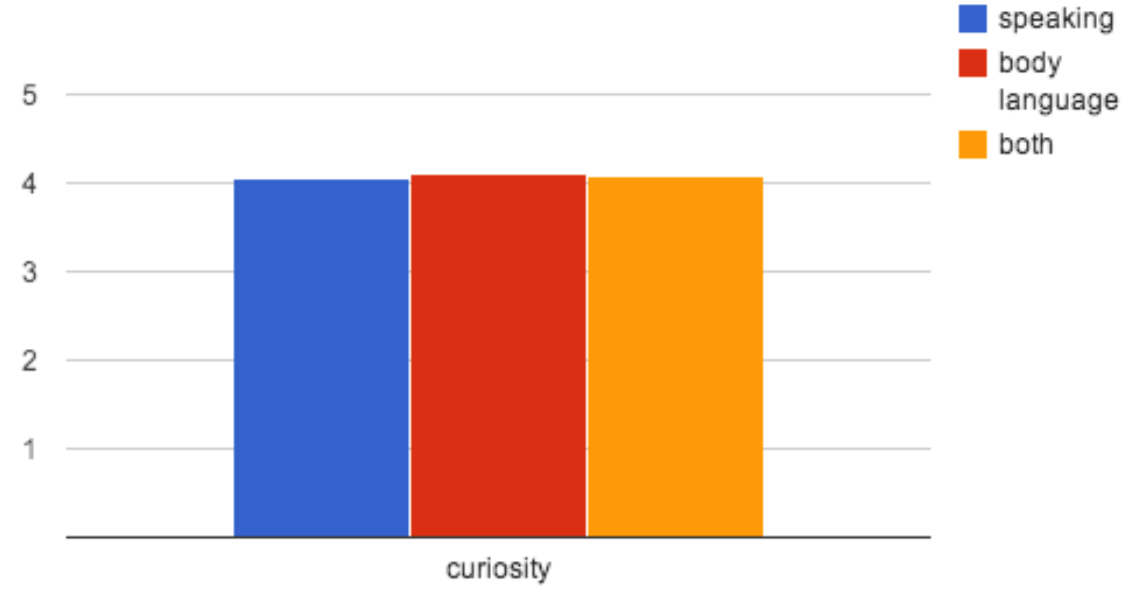
\includegraphics[width=0.9\columnwidth]{Figures/US_Curi_Dif.png}
% \caption{Different Language Group}
% \label{fig:US_Curi_Dif}
% \end{figure}


\subsubsection{Positive and Negative Co-experience}

\begin{figure}[!t]
\centering
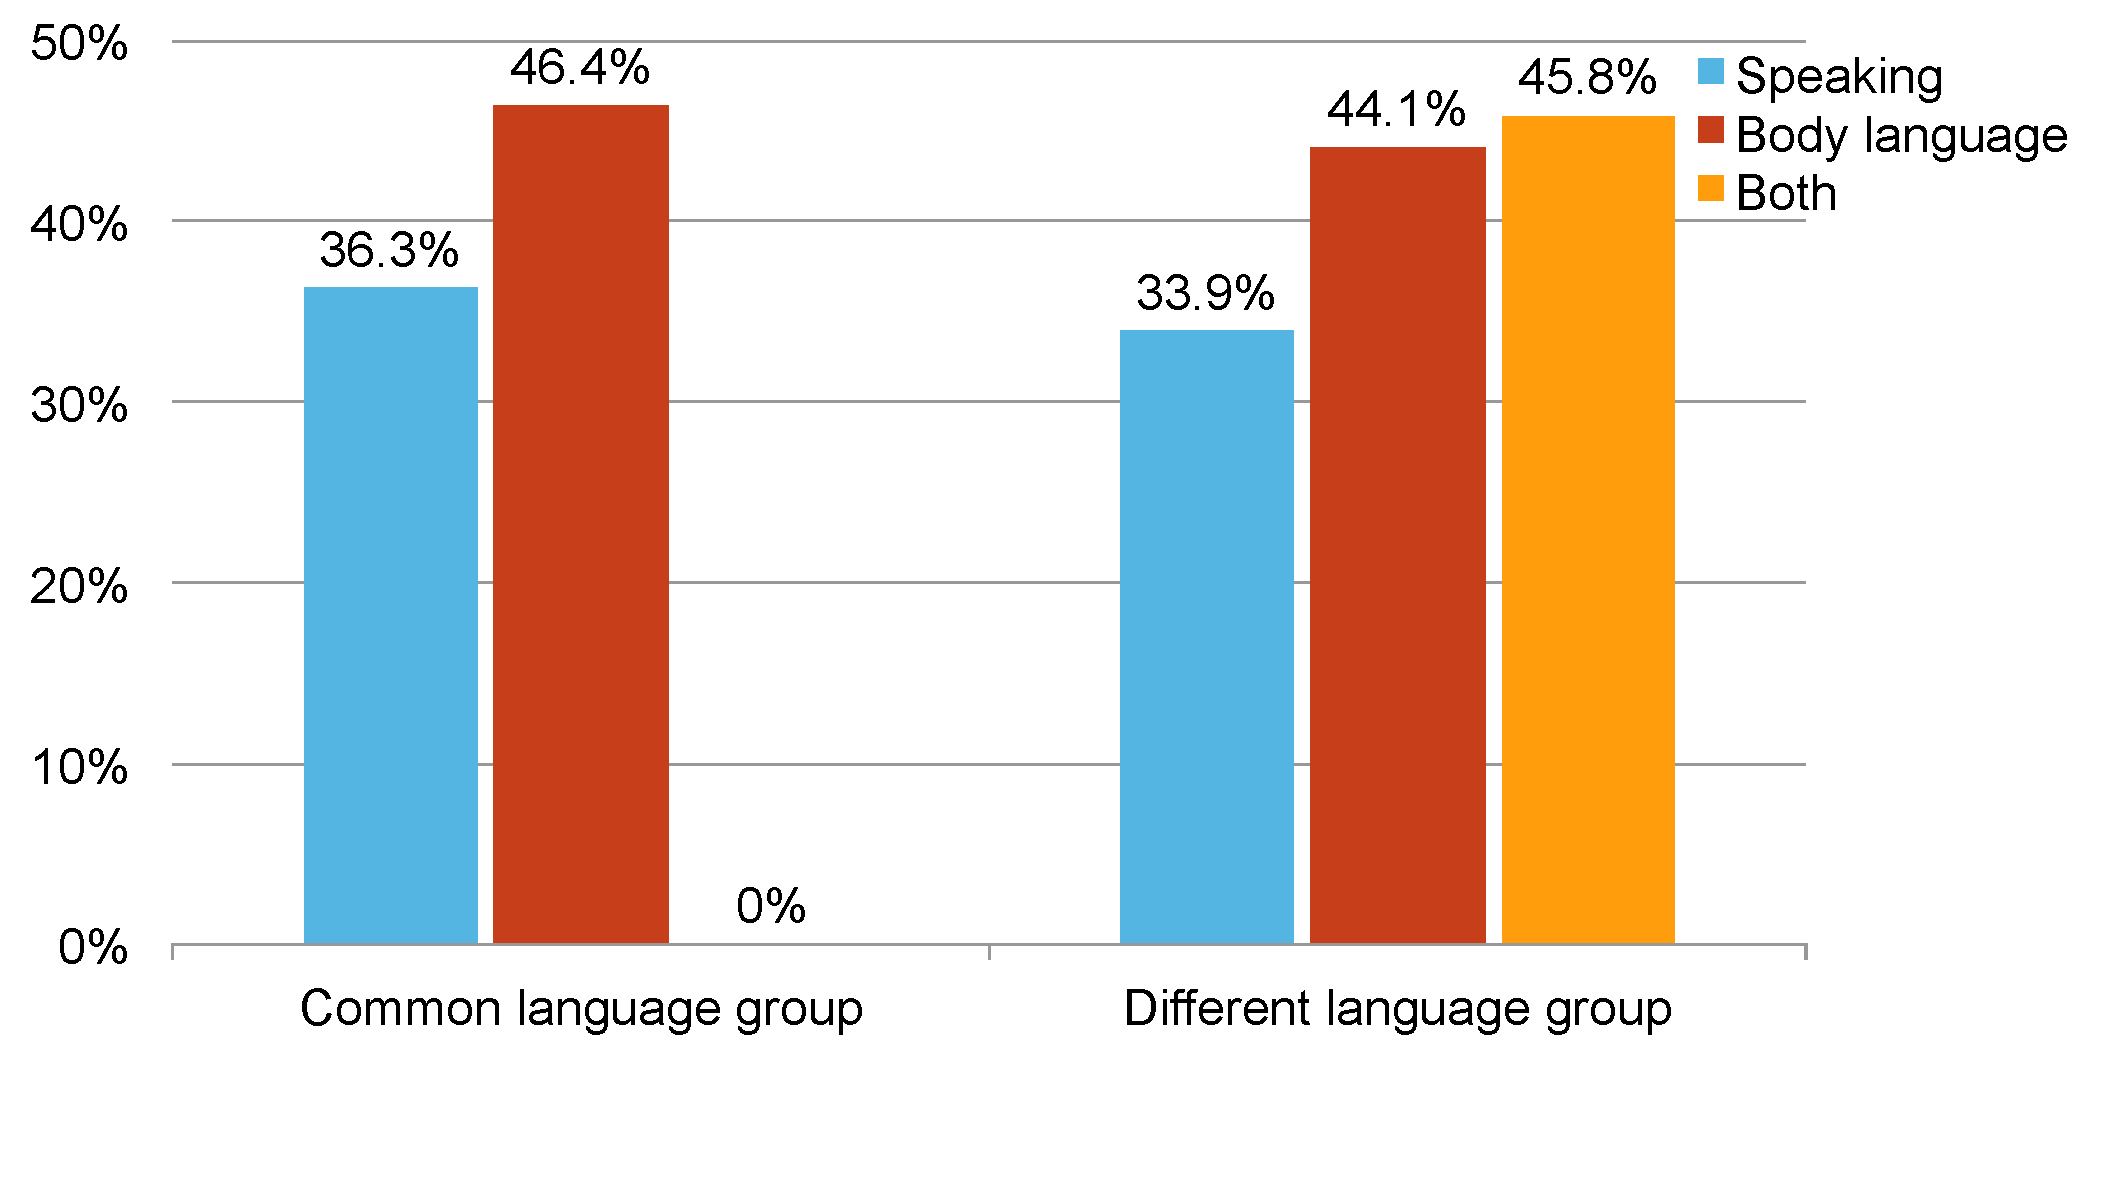
\includegraphics[width=0.8\columnwidth]{Figures/US_eSFQ_Pos_Average.pdf}
\caption{eSFQ: average co-experience of positive indexes (Cooperative, Happy, Fun, Fair, Encouraging, Triumphing, Satisfying).}
\label{fig:US_eSFQ_Pos_Average}
\end{figure}

\begin{figure}[!t]
\centering
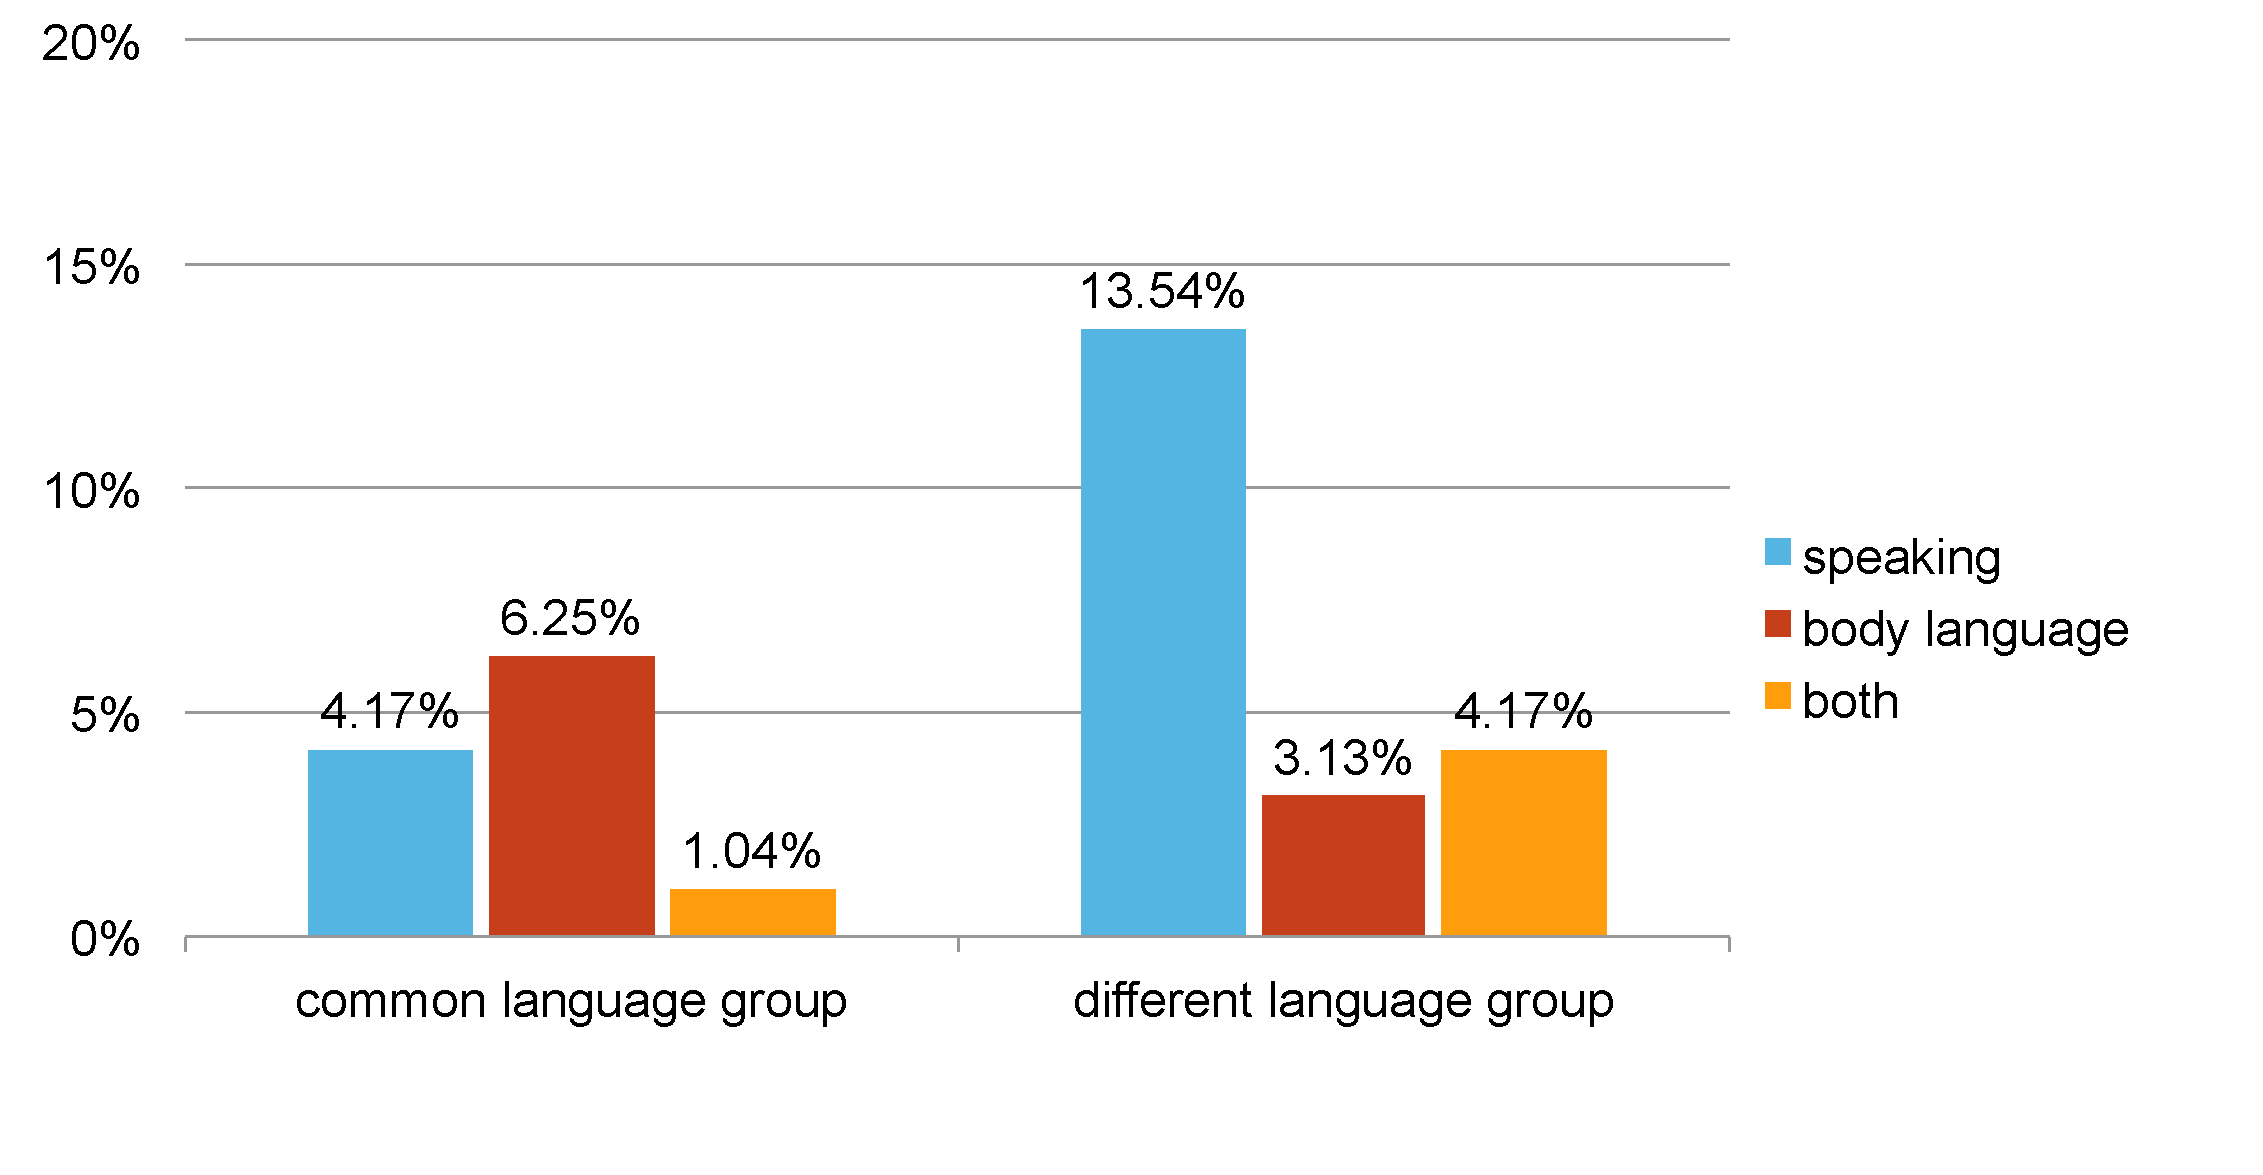
\includegraphics[width=0.8\columnwidth]{Figures/US_eSFQ_Neg_Average.pdf}
\caption{eSFQ: average co-experience of negative indexes (Defeat, Angry, Frustrating, Boring).}
\label{fig:US_eSFQ_Neg_Average}
\end{figure}

% \begin{figure}[!h]
% \centering
% 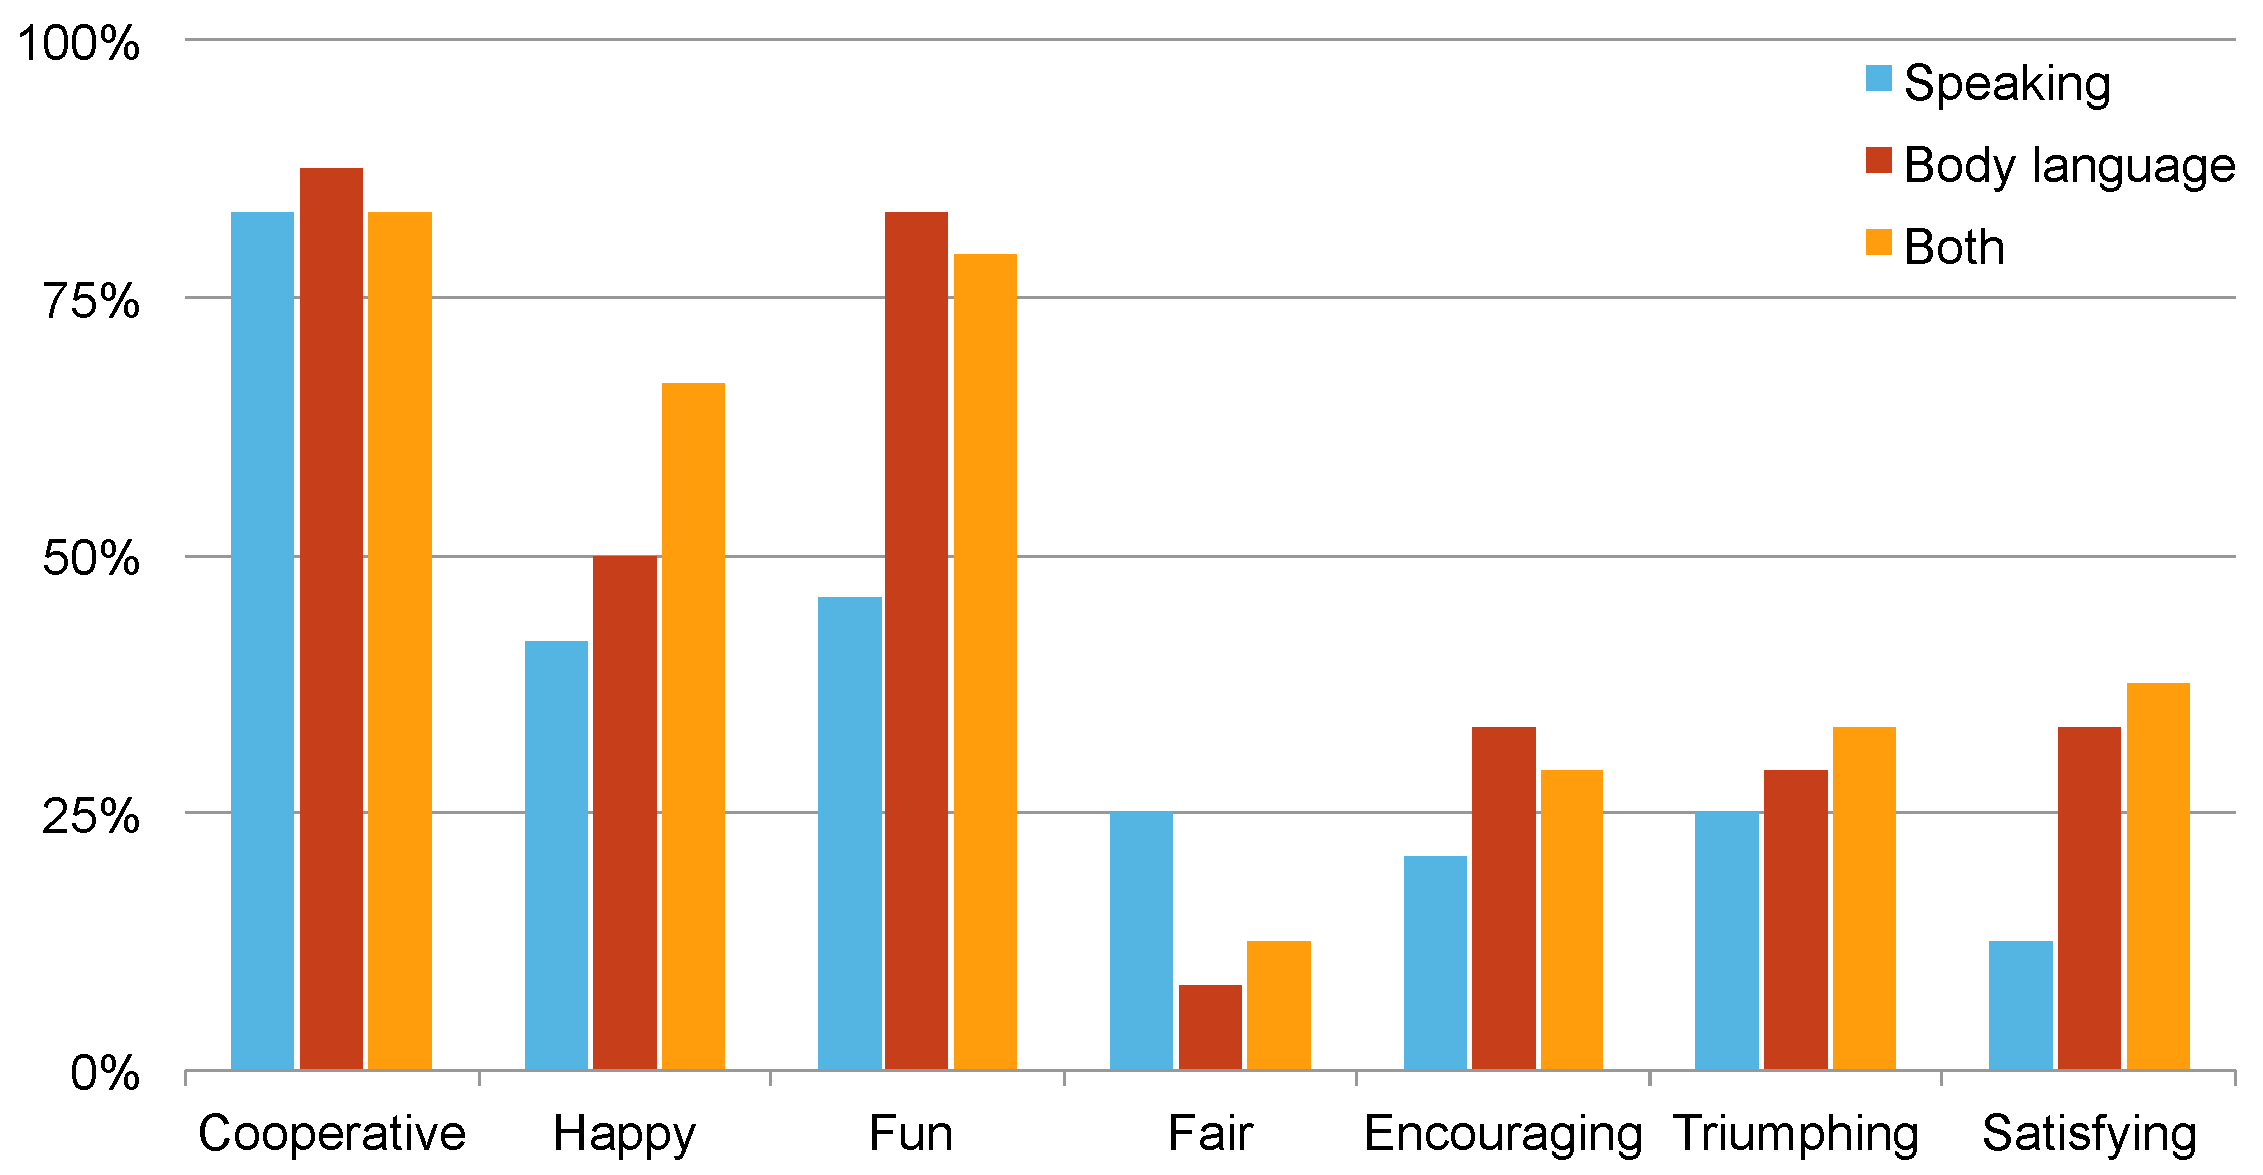
\includegraphics[width=0.9\columnwidth]{Figures/US_Co-ex_Com_Pos.pdf}
% \caption{Positive co-experience indexes for common language group.}
% \label{fig:US_Co-ex_Com_Pos}
% \end{figure}

% \begin{figure}[!h]
% \centering
% 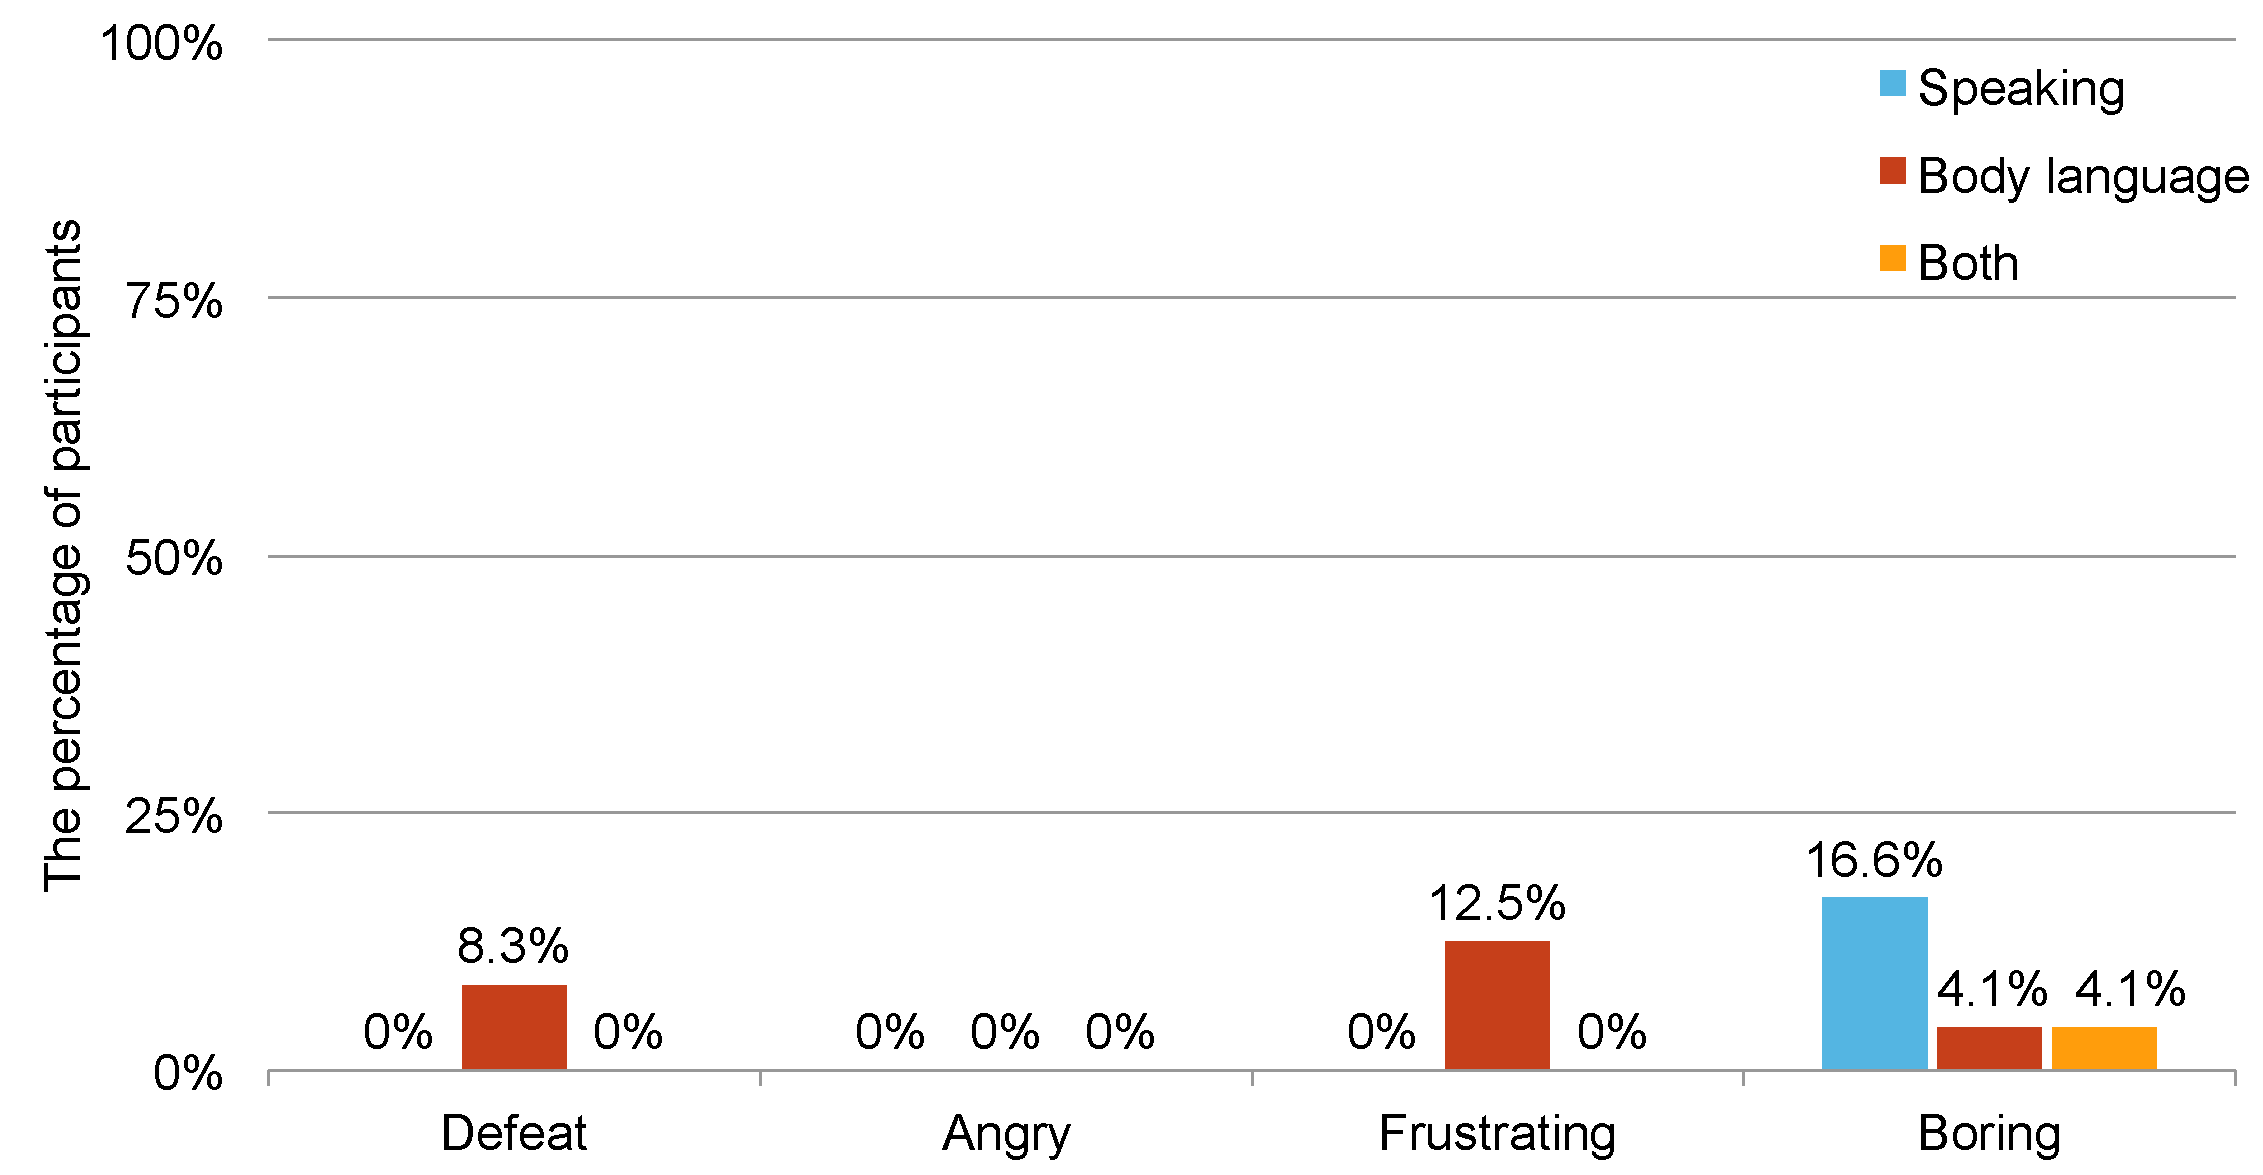
\includegraphics[width=0.9\columnwidth]{Figures/US_Co-ex_Com_Neg.pdf}
% \caption{Negative co-experience for common language group.}
% \label{fig:US_Co-ex_Com_Neg}
% \end{figure}


Figure~\ref{fig:US_eSFQ_Pos_Average} shows the average positive co-experience indexes for players with and without common languages. The positive co-experience is higher for communication modes with body language. Compared to speaking-only mode, adding body language 
improved positive co-experience by an average of 31\% and 33\% for players with and without common languages, respectively.

Figure~\ref{fig:US_eSFQ_Neg_Average} shows the average negative co-experience indexes for players with and without common languages. Compared to speaking-only mode, adding body language 
improved negative co-experience by an average of 13\% and 73\% for players with and without common languages, respectively.

%For common language group, the users experienced playing ``Speaking'' together as cooperative (83\% of the users), fun (46\%) and happy (42\%). The users experienced playing ``Body language'' together as cooperative (88\% of the user), fun (83\%), happy (50\%), encouraging (33\%) and satisfying (33\%). The users experienced playing ``Both'' together as cooperative (83\% of the user), fun (79\%), happy (67\%), satisfying (38\%) and triumphing (33\%).

%For different language group,the users experienced playing ``Speaking'' together as cooperative (83\% of the users), fun (54\%), happy (50\%) and frustrating (25\%). The users experienced playing ``Body language'' together as cooperative (79\% of the user), fun (67\%), happy (58\%), satisfying (54\%) and frustrating (13\%). The users experienced playing ``Both'' together as cooperative (88\% of the user), fun (88\%), happy (58\%), satisfying (46\%) and frustrating (13\%). 


\begin{figure}[!b]
\centering
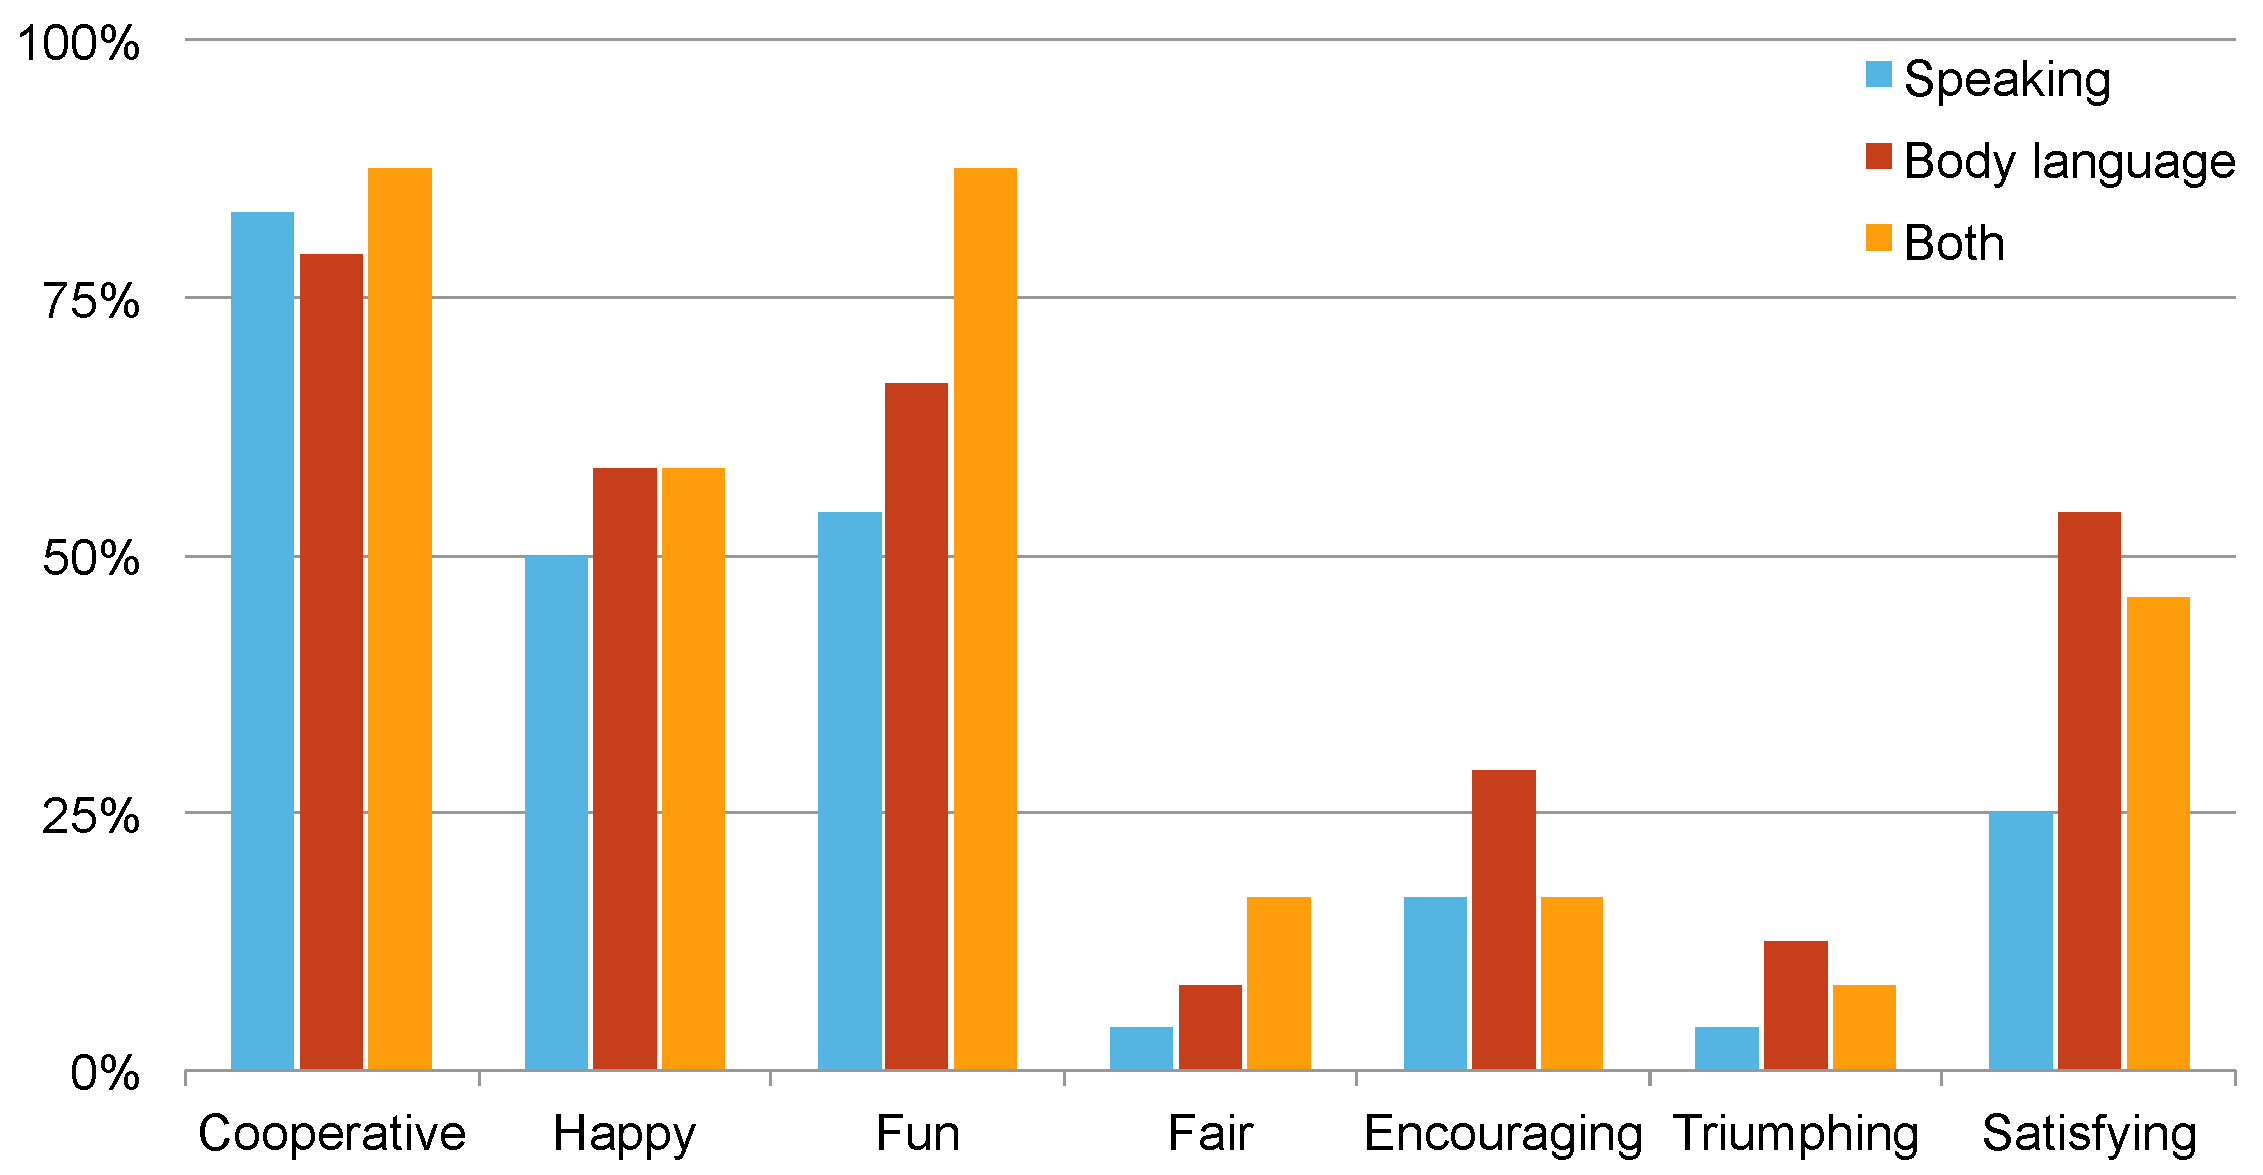
\includegraphics[width=0.9\columnwidth]{Figures/US_Co-ex_Dif_Pos.pdf}
\caption{Positive co-experience indexes for players without common languages.}
\label{fig:US_Co-ex_Dif_Pos}
\end{figure}

\begin{figure}[!t]
\centering
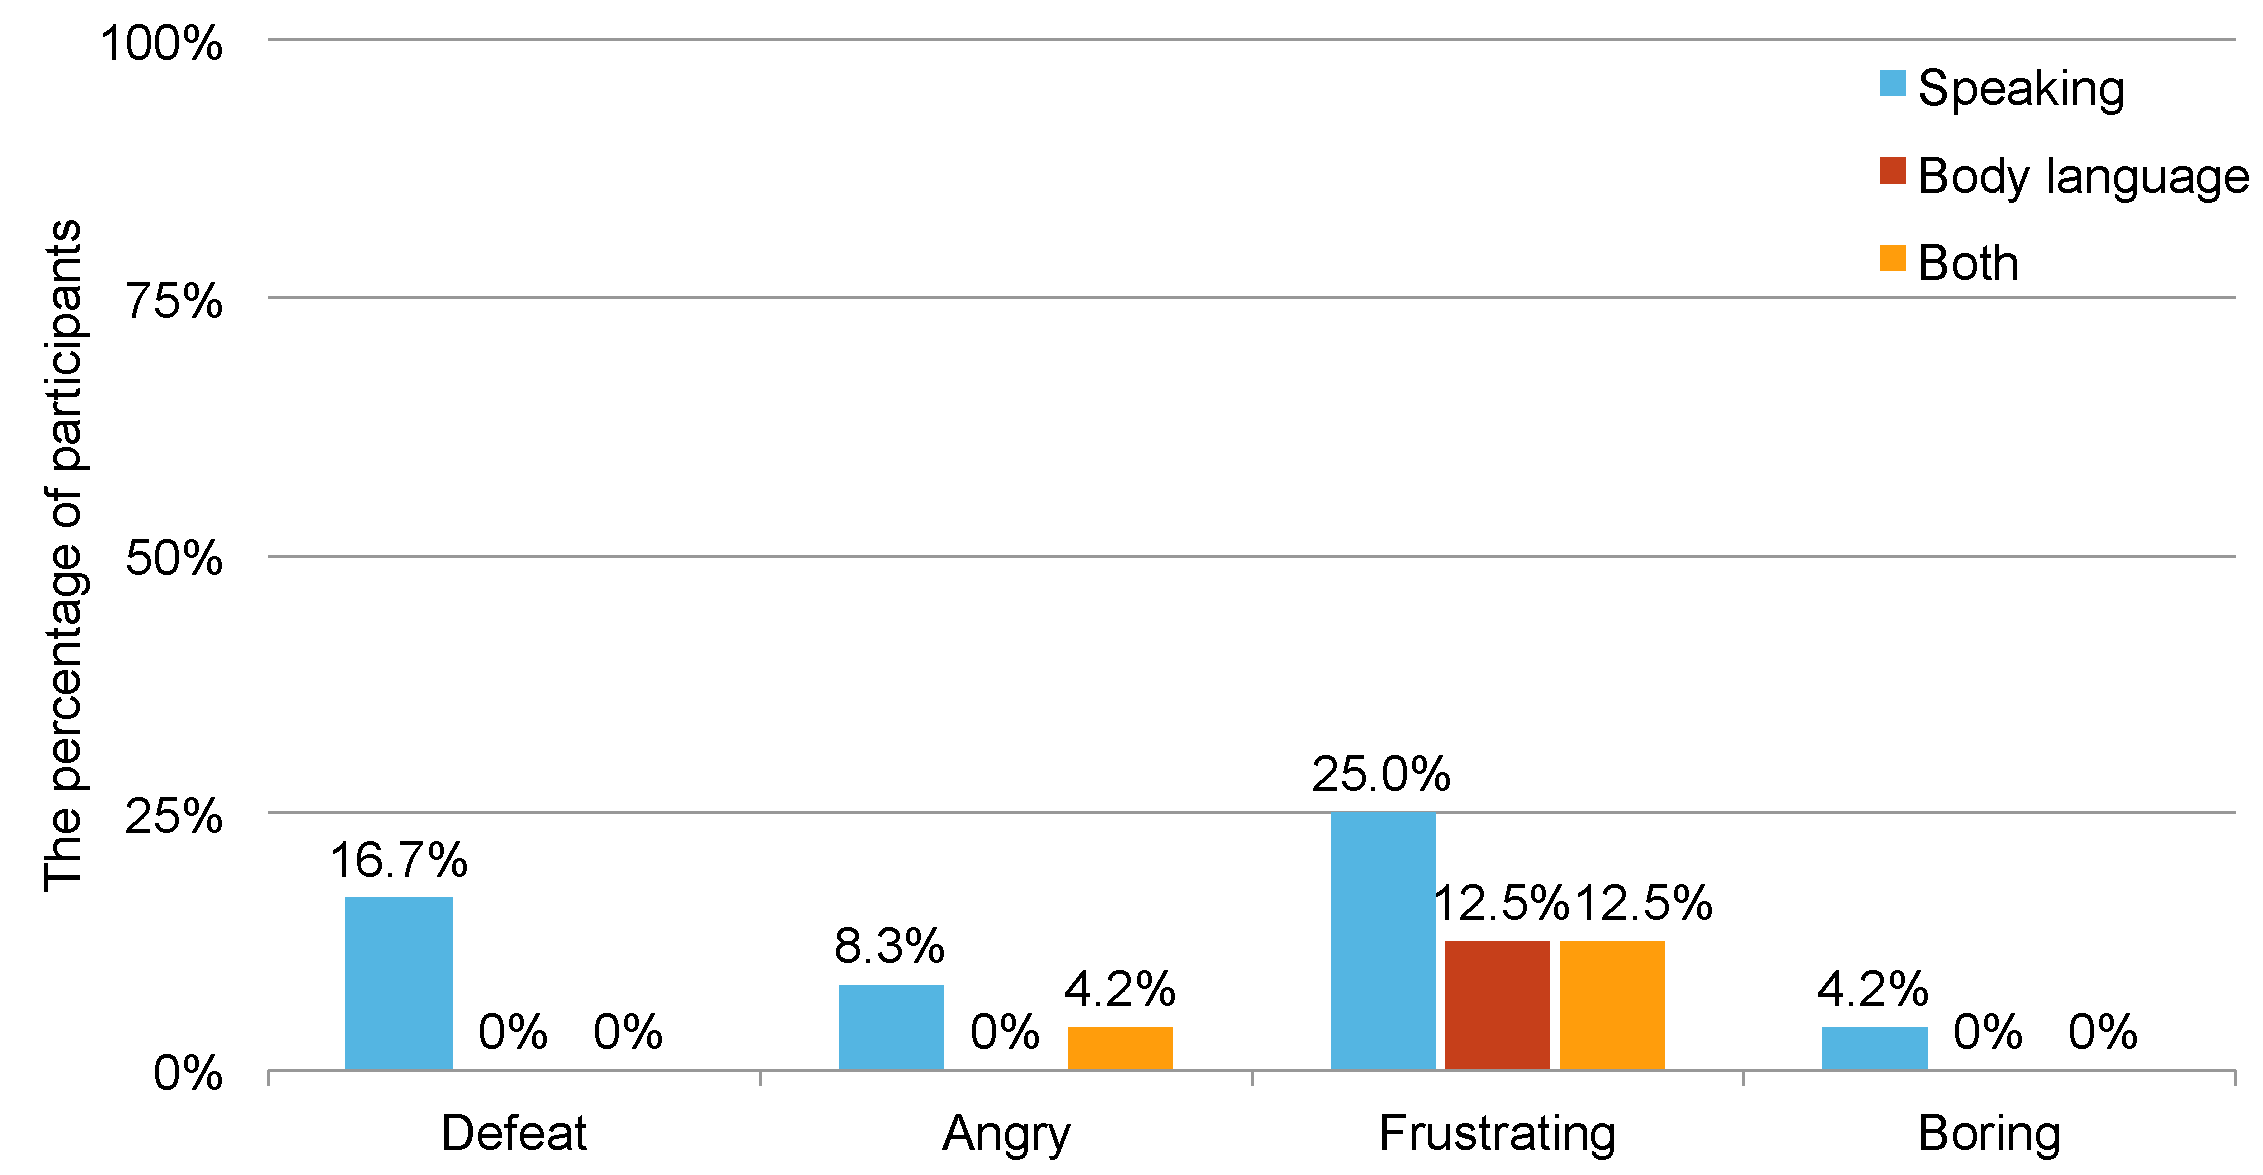
\includegraphics[width=0.9\columnwidth]{Figures/US_Co-ex_Dif_Neg.pdf}
\caption{Negative co-experience indexes for players without common languages (lower is better).}
\label{fig:US_Co-ex_Dif_Neg}
\end{figure}

Figure~\ref{fig:US_Co-ex_Dif_Pos} shows the individual positive co-experience indexes for players without common languages. Compared to speaking-only mode, we can see that all of these positive indexes increase when body language is added (except for cooperative in body language only mode). Specifically, satisfaction improved by an average of 99.5\%. 


% The co-experience rate ``Body language'' and ``using speaking and body langauge together'' were better than ``Speaking'', no matter in common language group or in different language group. In different language group, ``Speaking'' made 25\% people feel frustrated, and both ``Body language'' and ``using speaking and body language togther'' are 13\%.

% According to Figure~\ref{fig:US_Co-ex_Com_Pos}, ``Body language'' communication manner has the highest fun index for common language group. In accordance with Figure~\ref{fig:US_Co-ex_Dif_Pos}, ``Both'' communication manner has the highest fun index for different language group. However, from Figure~\ref{fig:US_Co-ex_Dif_Neg}, compared to traditional setting and body language setting, the frustrating rate decreases obviously from 25\% to 13\%, which means the ratio of frustrating decreased 48\%.

%According to the results, ``Body language'' communication manner has the highest fun index for common language group. And in accordance with Figure~\ref{fig:US_Co-ex_Dif_Pos}, ``Both'' communication manner has the highest fun index for different language group. However, from 

Figure~\ref{fig:US_Co-ex_Dif_Neg} shows the individual negative co-experience indexes for players without common languages. Compared to speaking-only mode, we can see that all of these negative indexes decrease when body language is added. Specifically, defeat and boring dropped from 16.7\% to zero, and frustration improved by an average of 48\%. 

%compared to traditional setting and body language setting, the frustrating rate decreases obviously from 25\% to 13\%, which means the ratio of frustrating decreased 48\%.


\subsection{Cooperative Performance Metrics (CPM) Results}

Cooperative Performance Metrics (CPM)\cite{CPMs} is designed to analyze cooperative gaming experience, typically through manual coding of the video recordings of players' facial expression (e.g. laughter) and body movement. CPM counts the occurrences of the following six types of co-behavior: ``Laughter or excitement together'', ``Work out strategies'', ``Helping each other'', ``Global Strategies'', ``Waited for each other'' and ``Got in each other's way ''.
Because `Global Strategies'' and ``Got in each other's way'' do not apply to our game, they are not shown in the subsequent analysis.

% Because the index of ``Laugher or excitement together'' is unfair to body language communicatin manner, which can't hear another player's sound, thus we added an additinal index: ``Laugher or excitement'', which indicates count of personal user's laugh times, and 


% Furthermore, for each CPM label within the video analysis, the researcher identified a cause based on the cooperative design patterns. Thus, before discussing our results, we will discuss the validation process we performed to evaluate the reliability of the results. First, to establish face validity, patterns and CPMs were developed through an intensive review process. To establish the scientific validity, we performed a formal validation process. We asked two independent researchers to rate four sessions given the CPMs and the cooperative patterns identified. All researchers read the CPMs in detail and were shown an example of how to apply them using a video-taped gameplay session. Afterwards, they were given four videos of play session to analyze. We then perform inter-rater agreement and calculated kappa values\cite{Kappa1,Kappa2}. 

Before we started coding CPMs, we performed a formal validation process to ensure inter-rater consistency. We asked two independent researchers to understand CPMs in depth and were shown examples of how to apply them using video of a gameplay session. Afterwards, researchers were given four videos to analyze and we calculated inter-rater agreement using kappa values\cite{Kappa1,Kappa2}. 

Table~\ref{tab:KappaValue} shows the results of our validation for each metric and for each of the sample videos. The lowest Kappa value, 0.75, is greater than 0.6 and is sufficient to establish validity. To further ensure accurate coding of CPMs, each of the 24-pairs of user study sessions was coded by oth researchers, and the results were averaged. 

% Table~\ref{tab:KappaValue} shows the results of this process. Based on these results, the kappa value presented are sufficient to establish validity of the approach and the results (\textgreater 0.6 means highly consistent degree).

\begin{table}[!h]
\renewcommand\arraystretch{1.2}
  \centering
  \begin{tabular}{
  !{\vrule width2pt}m{0.15\columnwidth}
  !{\vrule width2pt}m{0.15\columnwidth}
  !{\vrule width2pt}m{0.17\columnwidth}
  % !{\vrule width2pt}p{0.15\columnwidth}
  % !{\vrule width2pt}p{0.08\columnwidth}
  % !{\vrule width2pt}p{0.08\columnwidth}
  %!{\vrule width2pt}p{0.08\columnwidth}
  %!{\vrule width2pt}p{0.08\columnwidth}
  %!{\vrule width2pt}p{0.08\columnwidth}
  !{\vrule width2pt}m{0.15\columnwidth}
  !{\vrule width2pt}m{0.15\columnwidth}
  !{\vrule width2pt}}
    \Xhline{2pt}
    \multicolumn{1}
    {!{\vrule width2pt}c!{\vrule width2pt}}
    {\tabhead{\multirow{2}{*}{Inter-rater}}} &
    %\multicolumn{6}
    \multicolumn{4}
    {c!{\vrule width2pt}}
    {\centering\tabhead{Kappa for Metrics}} \\
    \Xcline{2-5}{2pt}
    % \hline
    %& M1 & M2 & M3 & M4 & M5 & M6 \\
     & Laughter together & Work out strategies & Helping each other & Waited for each other\\
    \Xhline{2pt}
    %Session1 & 0.75 & 1 & 0.79 & - & 1 & - \\
    Session1 & 0.75 & 1 & 0.79 & 1\\
    \Xhline{2pt}
    %Session2 & 1 & 0.8 & 1 & - & 1 & - \\
    Session2 & 1 & 0.8 & 1 & 1\\
    \Xhline{2pt}
    %Session3 & 0.75 & 1 & 0.87 & - & 1 & - \\
    Session3 & 0.75 & 1 & 0.87 & 1\\
    \Xhline{2pt}
    %Session4 & 1 & 1 & 0.96 & - & 1 & - \\
    Session4 & 1 & 1 & 0.96 & 1\\
    \Xhline{2pt}
    %Average & 0.88 & 0.96 & 0.91 & - & 1 & - \\
    Average & 0.88 & 0.96 & 0.91 & 1\\
    \Xhline{2pt}
  \end{tabular}
  \caption{Inter-rater Agreement (M stands for CPM)}
  \label{tab:KappaValue}
\end{table}


\begin{figure}[!h]
\centering
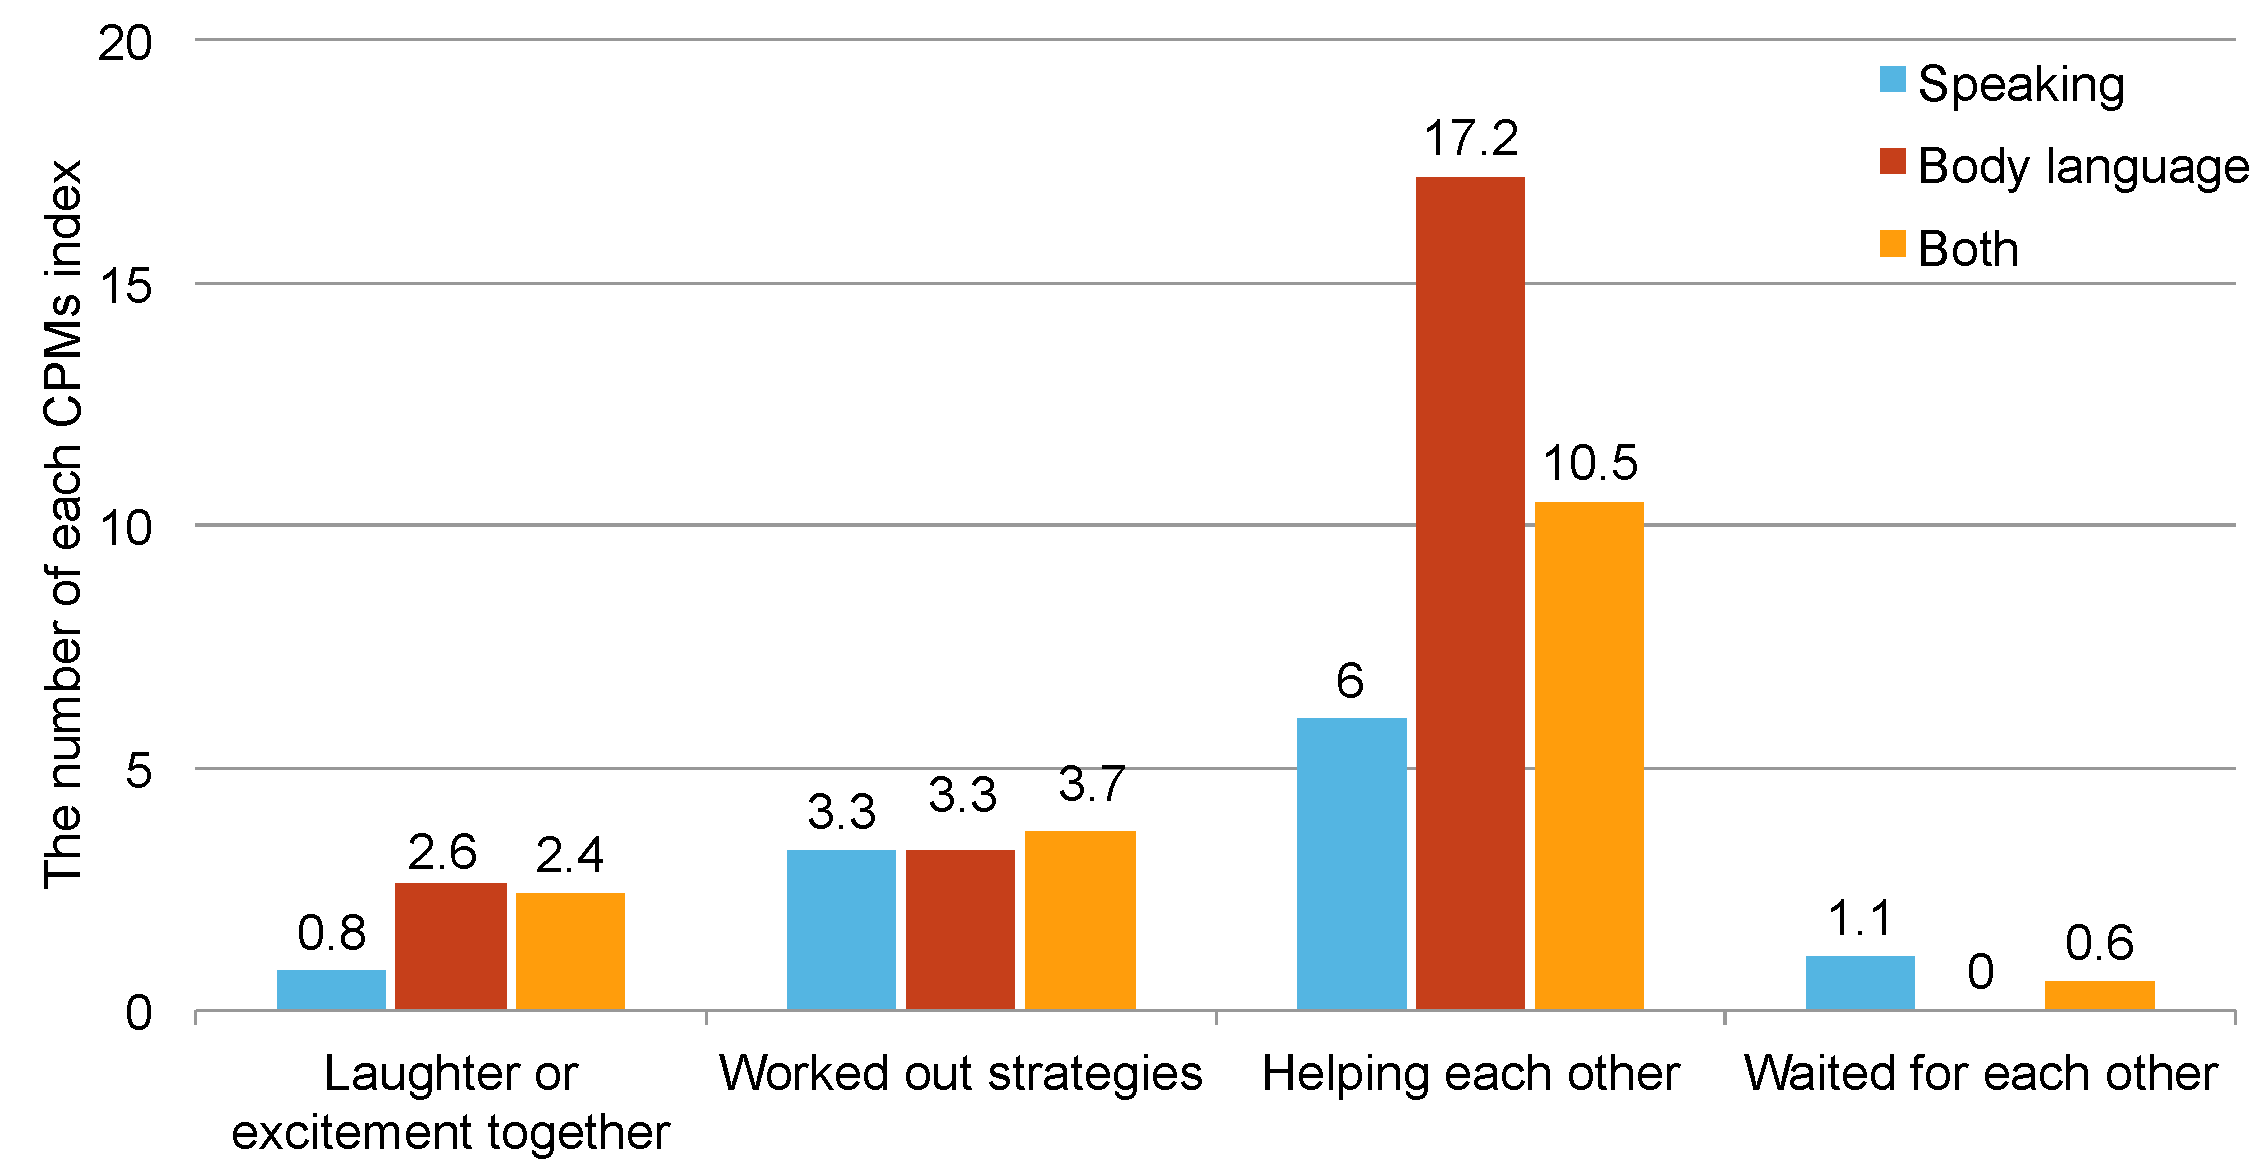
\includegraphics[width=0.9\columnwidth]{Figures/US_CPMs_Com.pdf}
\caption{CPMs result for players with common languages.}
\label{fig:US_CPMs_Com}
\end{figure}

\begin{figure}[!h]
\centering
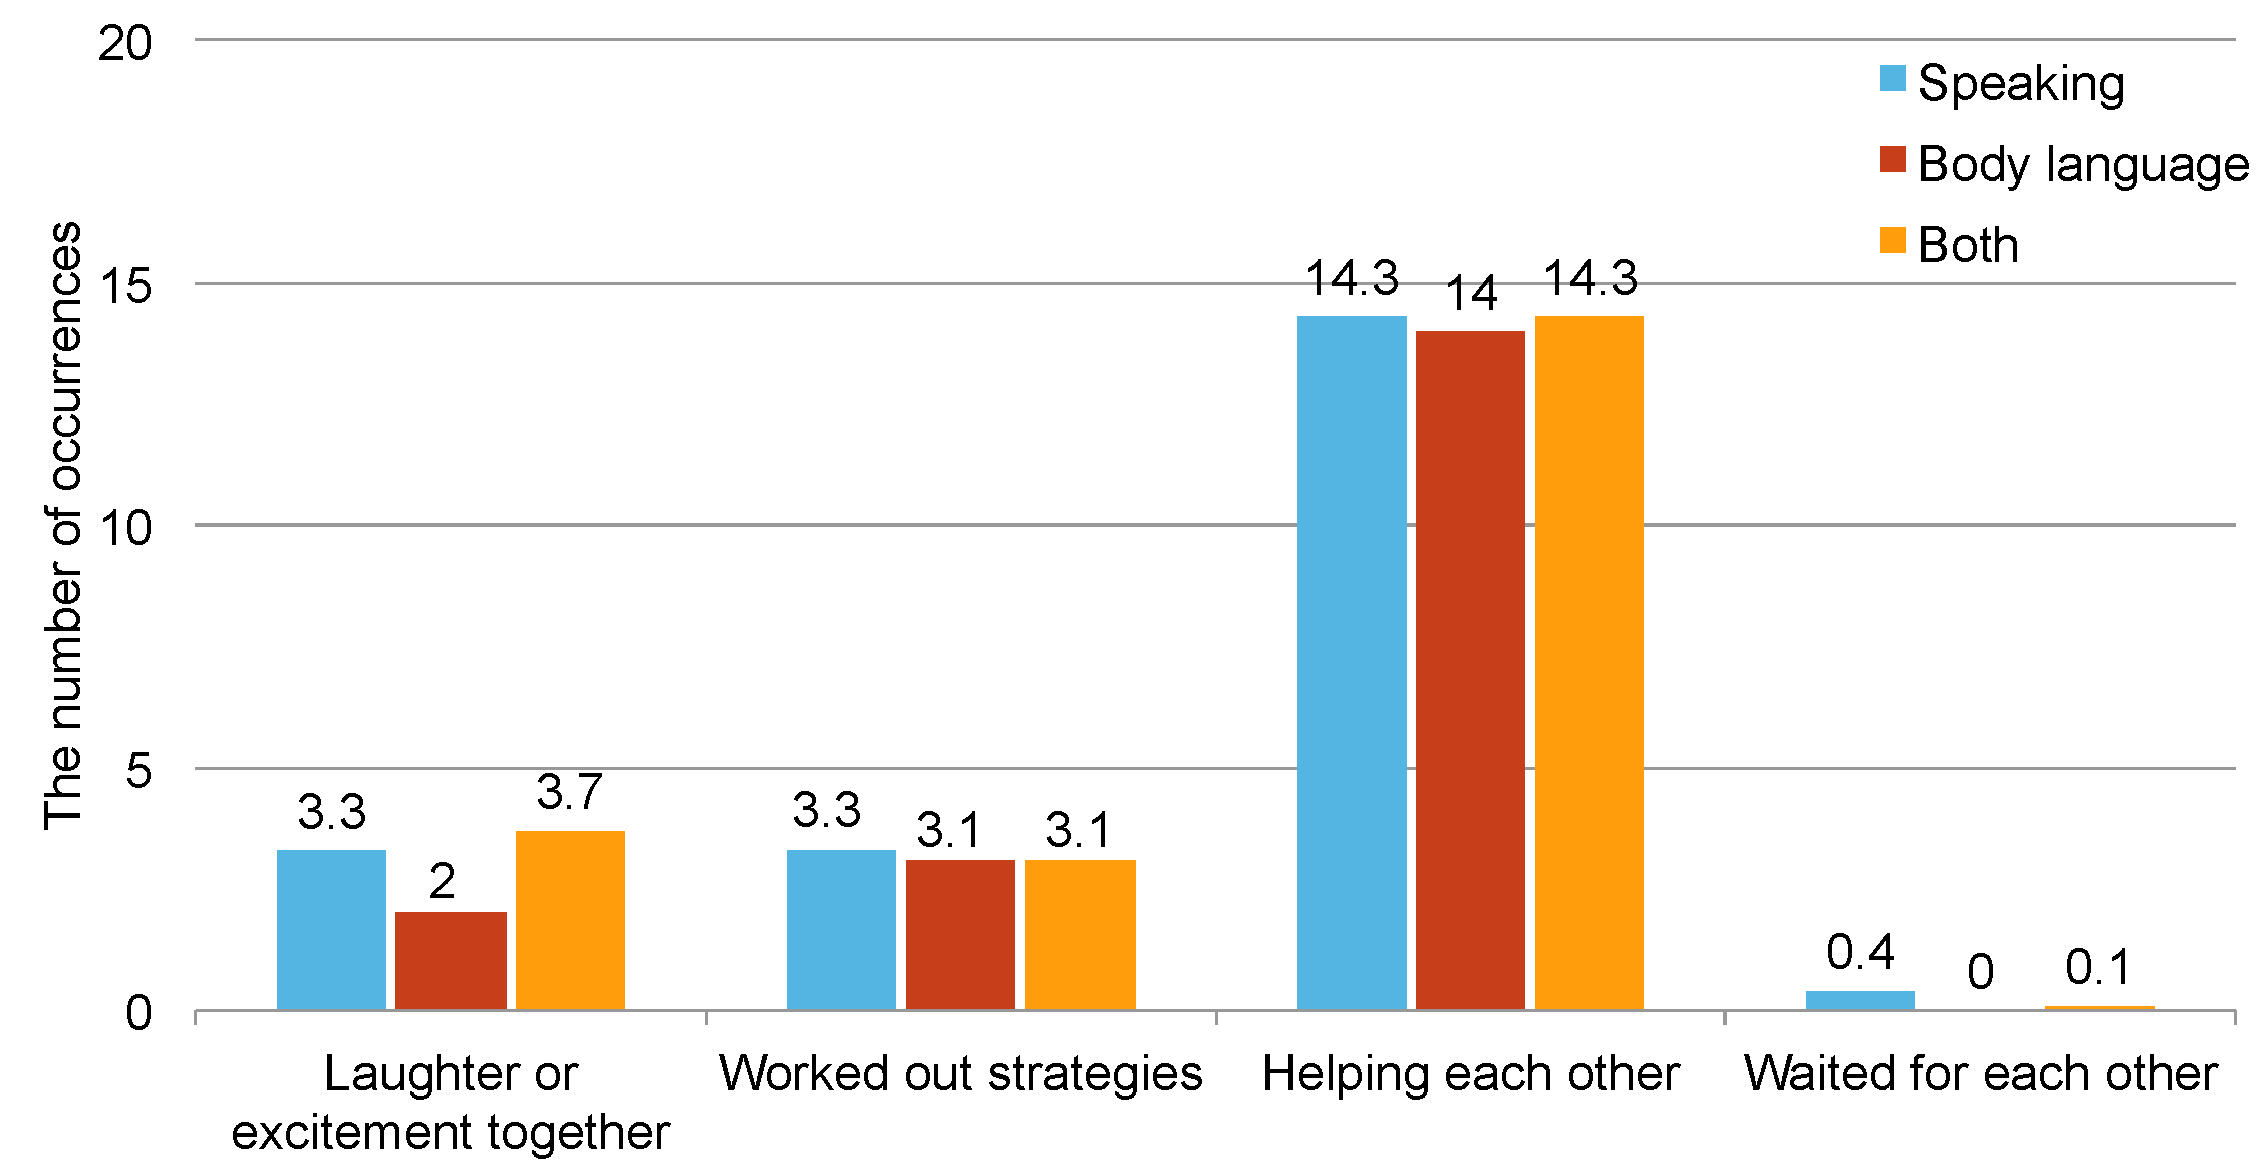
\includegraphics[width=0.9\columnwidth]{Figures/US_CPMs_Dif.pdf}
\caption{CPMs result for players without common languages.}
\label{fig:US_CPMs_Dif}
\end{figure}

Figure~\ref{fig:US_CPMs_Com} shows the CPM results for players with common languages. Compared to speaking only, adding body language communication increased ``laughter or excitement'' and ``helping each other''. ``Laughter or excitement'' increased because body language sometime led to unexpected and funny body movement. ``Helping each other'' increased because players were communicating with shorter but more frequent instructions, leading to more occurrences of helping each other being recorded. 

Figure~\ref{fig:US_CPMs_Dif} shows the CPM results for players without common languages. 
``Laughter or excitement'' was lowest for the body language mode.  We observed funny sounds and tones the players would make, such as when someone fumbled and made a clumsy mistake, and would lead to laughter. Also, laughter by one player was often mirrored by the other player. 

%, ``Speaking'' and ``Both'' communication manner cause more ``laughter or excitement''. We concluded that it is hard to trigger ``laugher or excitement'' without sound transmission. Compared to common language group and different langauge group, it shows that CPMs index of body language is similar, providing a consistent experience.

 
% after the integration of our data, we could find out that ``Body language'' occurred most frequently at CPMs indexes except index of ``Waited for each other''. Second is ``using speaking and body language together'', and ``Speaking'' occurred least frequently. Furthermore, ``Helping each other'' and ``Laugher or excitement'' were in direct proportion. And ``Helping each other'' increased significantly while using body language communication manner.

% from the count of each index happened, we could conclude that ``using speaking and body language together'' had highest frequency to happen. Second is ``Speaking'', and ``Body language'' had lowest frequency to happen. In addition, making comparison between different language group and common language group, count of ``Helping each other'' of different language group increased significantly in ``Speaking'' and ``using speaking and body language together'', and count of all CPMs indexes happened in ``Body language'' were almost the same for common language group.



\subsection{Final Questionnaire Results}
Our final questionnaire asked the preferences among the communication modes: ``Favorite'', ``Most fun'', ``Easiest'', ``Most difficult'', ``Most intuitive'', and ``Most cooperative''.
%communication manners respectively with ``Speaking'', ``Body language'' and ``Both'' three distinct choice.


%\subsubsection{Players With Common Languages}


\begin{figure}[!t]
\centering
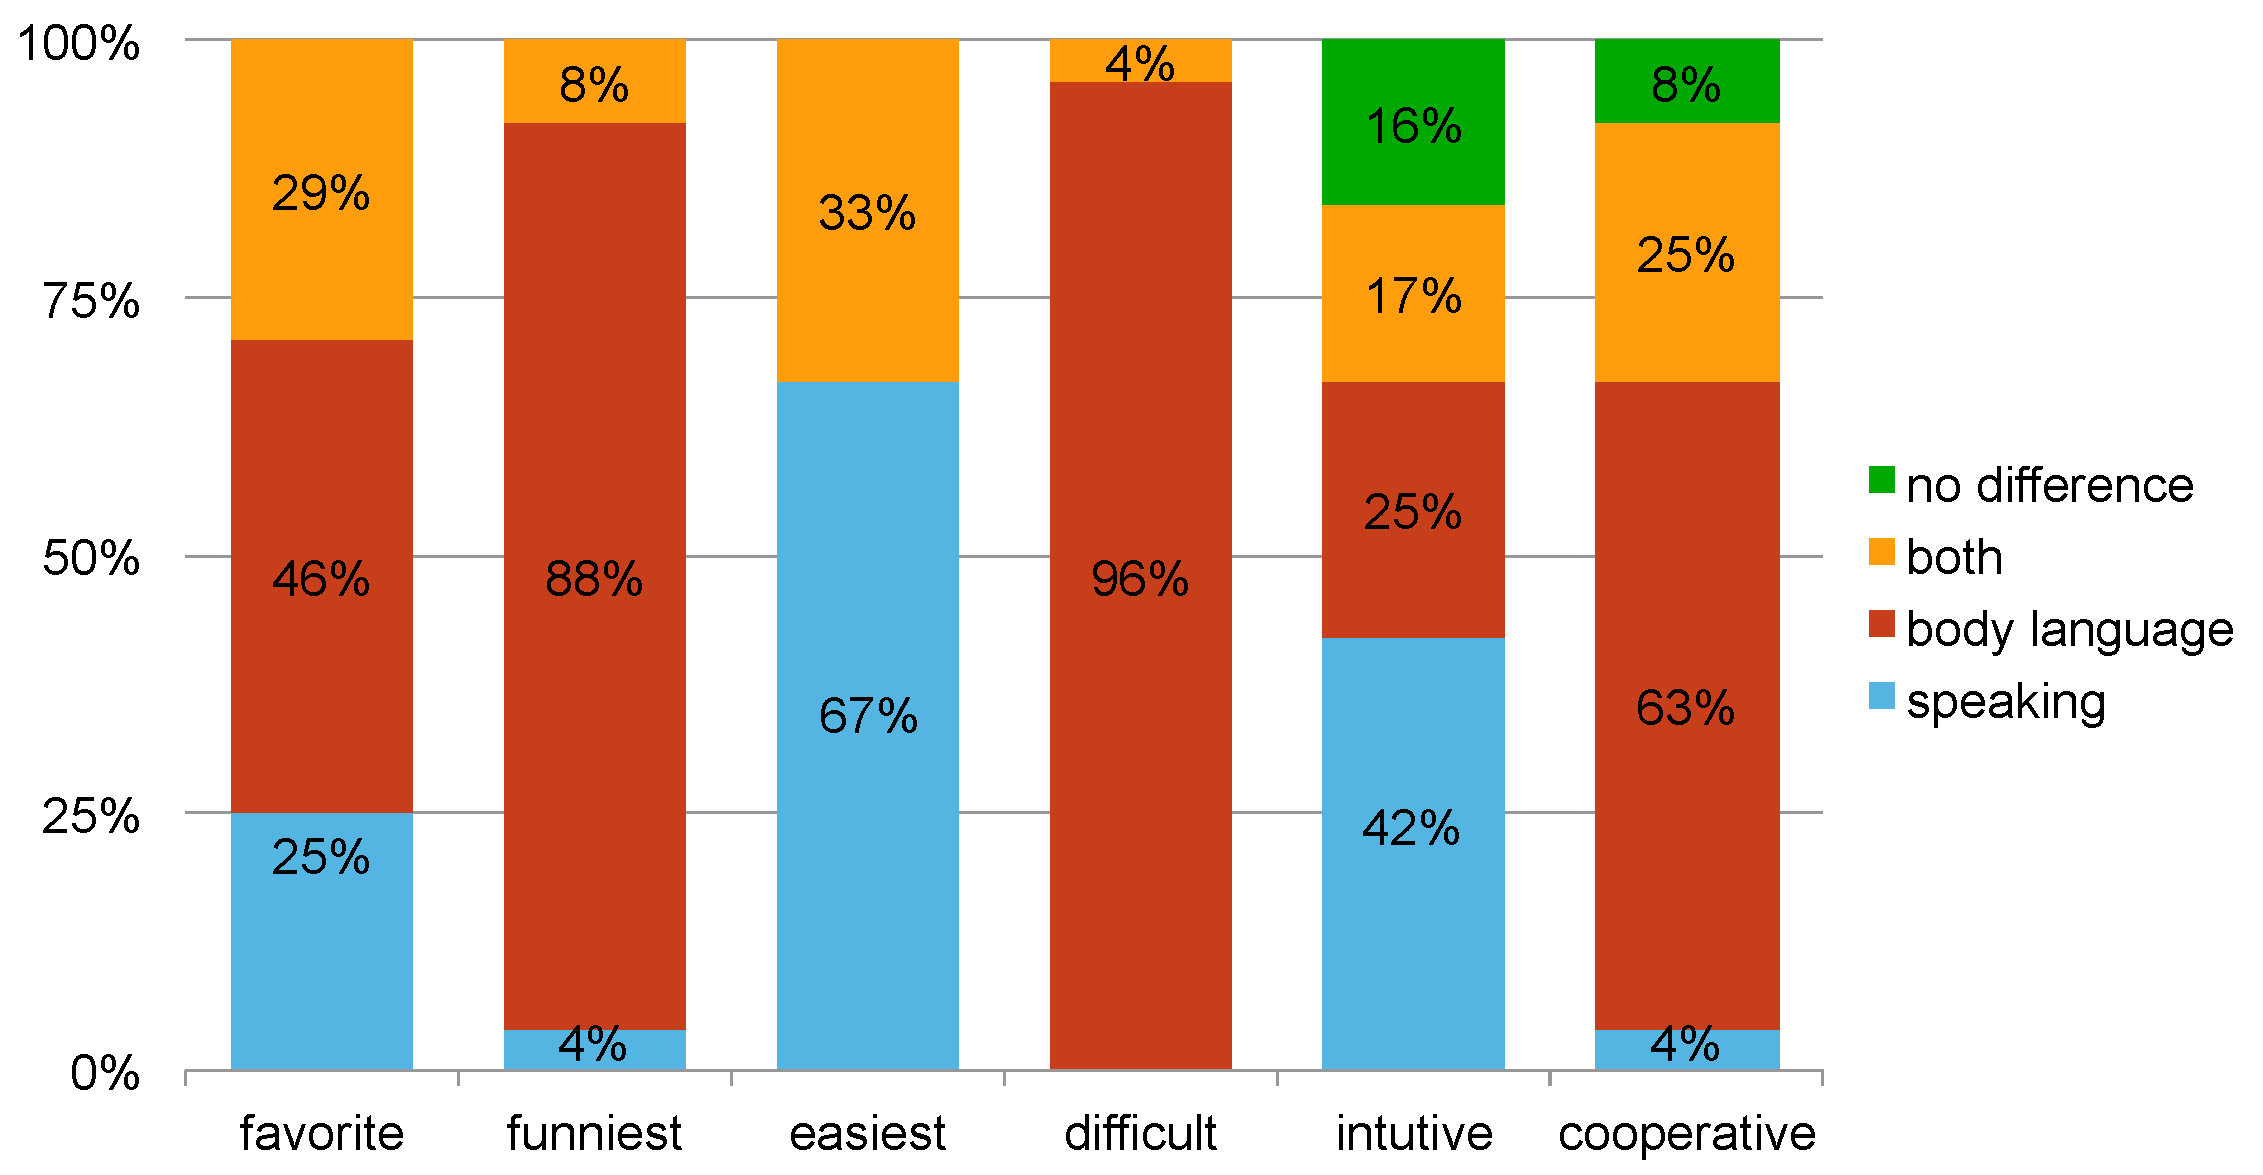
\includegraphics[width=0.9\columnwidth]{Figures/US_FQ_Com.pdf}
\caption{Overall preference for players with common languages.}
\label{fig:US_FQ_Com}
\end{figure}

Figure~\ref{fig:US_FQ_Com} shows the preferences for players with common languages. 
% We could find out that most users feel ``Body language'' is the most difficult one. However, 
Body language without speaking was found to be most difficult by 96\% of the players, yet had the highest proportion in the index of ``Favorite'' (46\%), ``Most fun'' (88\%), and ``Most cooperative'' (63\%). Using the GameFlow model shown in Figure~\ref{fig:GD_F1}, the experience in speaking mode may be boring, and the body language mode may lower the skill level and make the experience more fun.
% most people also felt ``Body language'' is the most interesting, the best cooperative feeling's, and the most favorite communication manner. Another communication manner, ``using speaking and body language together'', also have good expression. From our statistics, users considered that ``using speaking and body language together'' has better gameplay interesting and cooperative feeling's than ``Speaking''. 
%And more than half of users felt ``Speaking'' is the easiest, the most intuitive and the least interesting manner to communicate.


%\subsubsection{Players Without Common Languages}


\begin{figure}[!t]
\centering
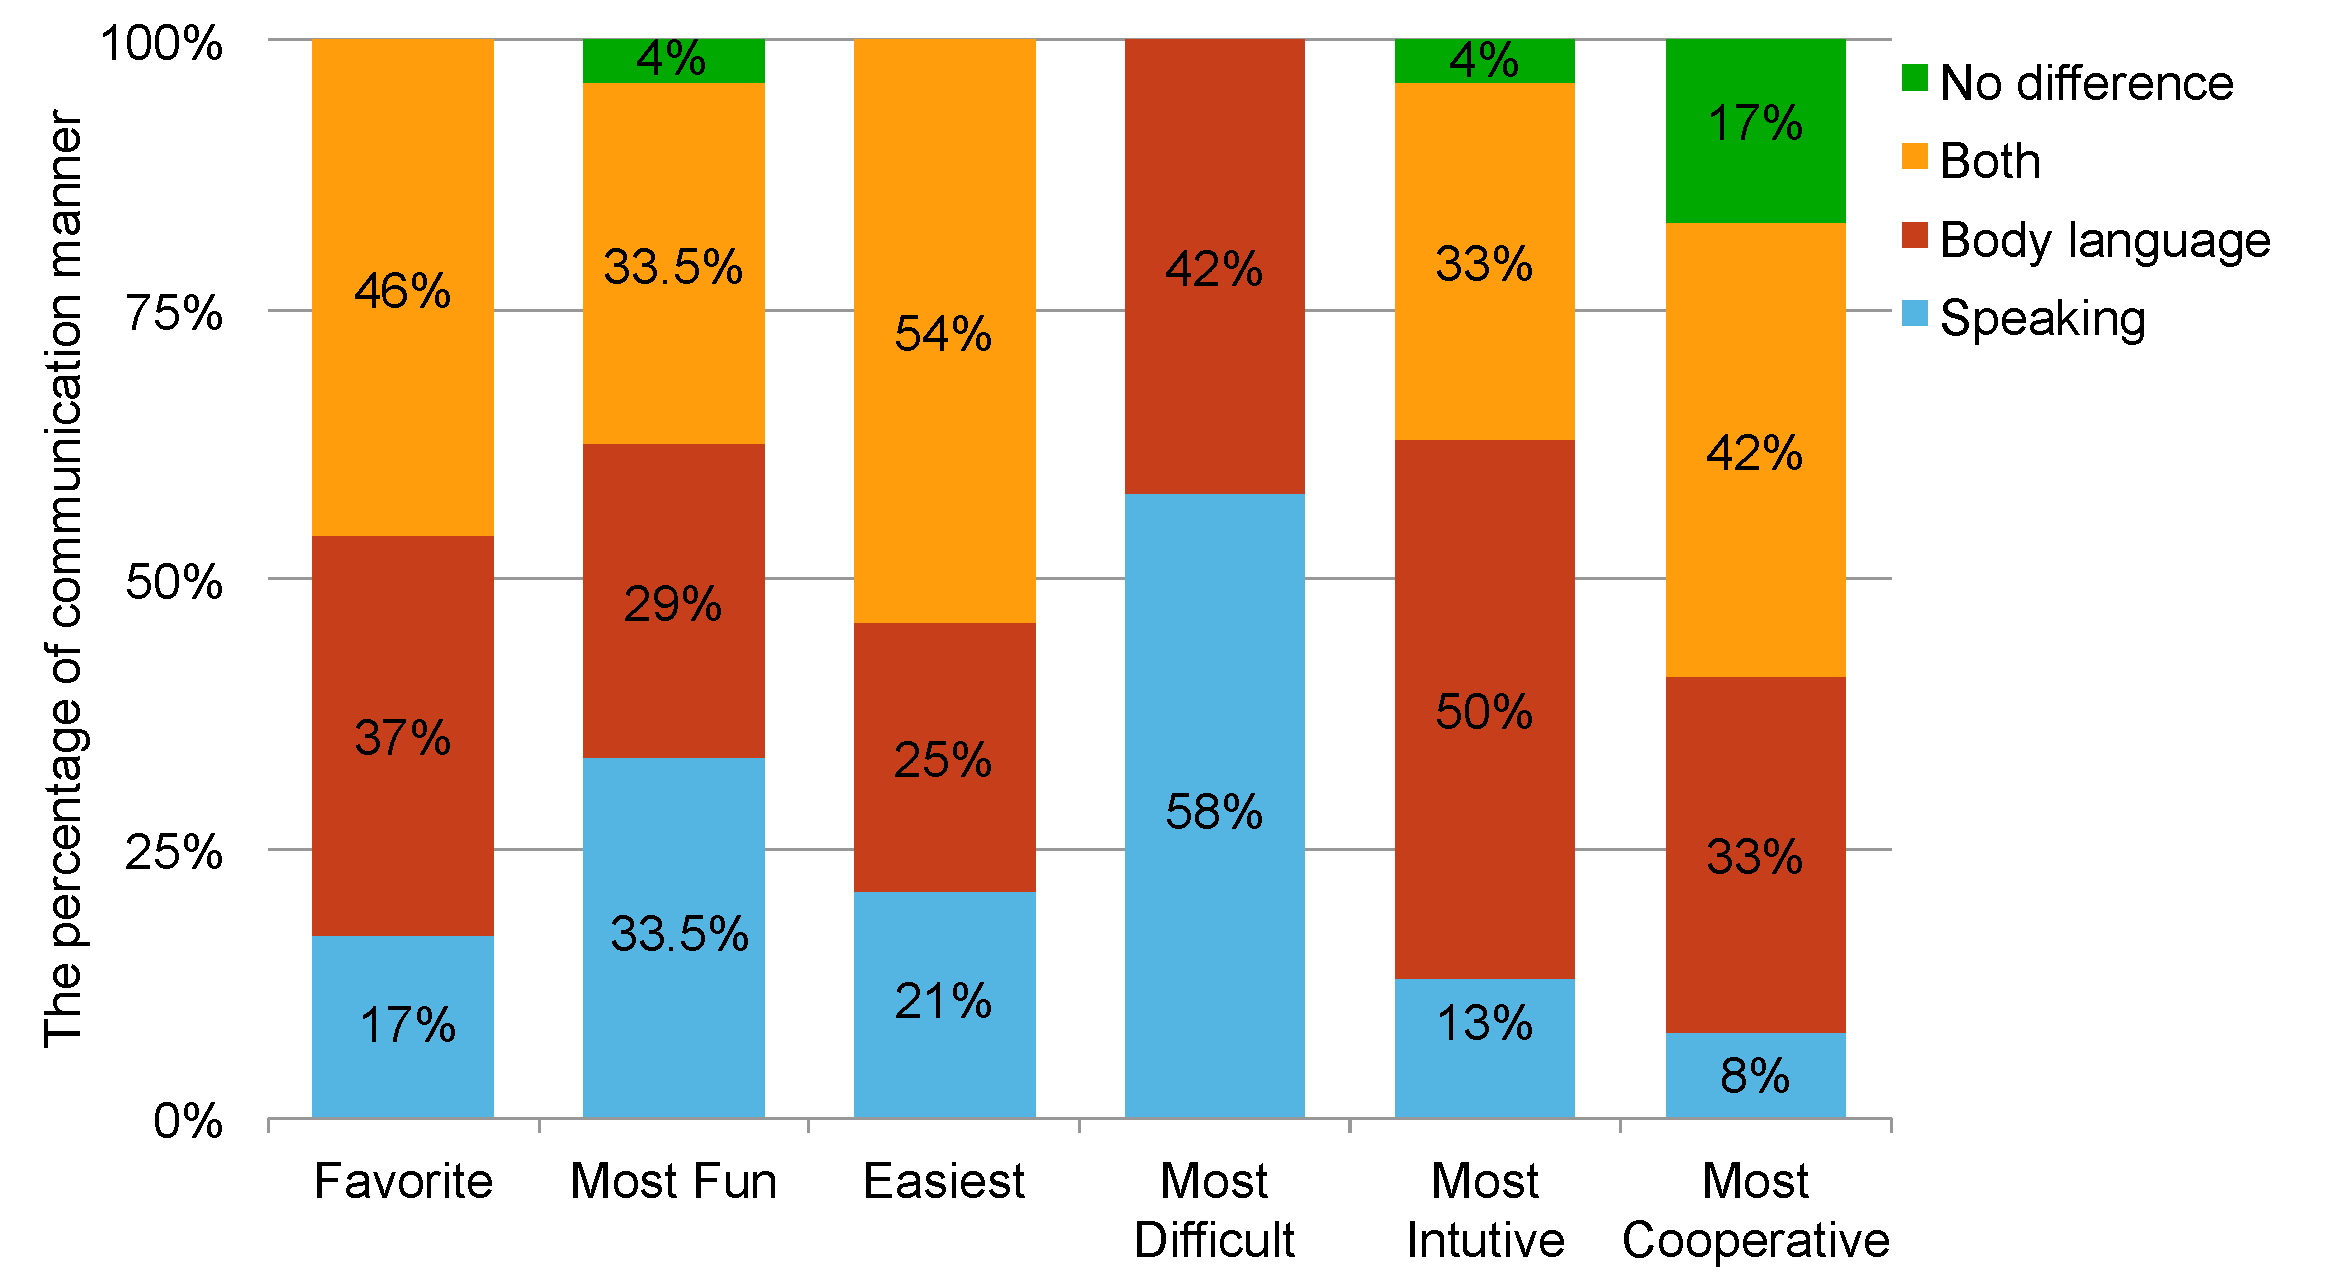
\includegraphics[width=0.9\columnwidth]{Figures/US_FQ_Dif.pdf}
\caption{Overall preference for players without common languages.}
\label{fig:US_FQ_Dif}
\end{figure}

Figure~\ref{fig:US_FQ_Dif} shows the preferences for players without common languages.
Most of the users (58\%) found the speaking mode as the most difficult, and found the body-language mode as the most intuitive (50\%). Most users preferred using both speaking and body language together (46\%) and found it ``Most fun'' (33.5\%), ``Easiest'' (54\%), and ``Most cooperative'' (42\%).


% and the difficulty and interesting proportion had increased significantly to compare with common language group. 
% Nonetheless, the ratio of favorite and intuitive decreased, which could be explained that user felt not intuitive to use speaking language to communicate if both player were original in different language group. In addition, the cooperative feeling didn't have obvious increase. 
%Most users thought that ``Both'' communication manner was the easiest, the best cooperative feeling's and the most favorite communication manner. We could find out that although it was easy, but most player still felt fun. ``Body language'' remained a great gameplay experience and most players thought that it's the most intuitive manner to communicate when we have language boundary with the other player.


\section{Discussion}

\subsection{Consistency in Game Experience}

% As we can see in Figure~\ref{fig:US_Consistent} and Table~\ref{tab:Consistency}, we can observe that, with traditional setting (speaking), the eSFQ and CPMs index patterns are inconsistent(the average difference is 22.40\% and 2.90 times). In other words, it's a different game expereience. However, with our body language communication manner design, the eSFQ and CPMs index patterns are similar(the average difference is 6.25\% and 1.00 time). It implies cooperative game has more consistent game experience with body language communication.



% \begin{table}[!h]
% \renewcommand\arraystretch{1.5}
%   \centering
%   \begin{tabular}{
%   !{\vrule width2pt}c
%   !{\vrule width2pt}c
%   % !{\vrule width2pt}c
%   !{\vrule width2pt}}
%     \Xhline{2pt}
%     \multicolumn{1}
%     {!{\vrule width2pt}c!{\vrule width2pt}}
%     {\tabhead{}} &
%     \multicolumn{1}
%     {c!{\vrule width2pt}}
%     {\centering\tabhead{average difference of eSFQ game experience}} \\
%     % \multicolumn{1}
%     % {c!{\vrule width2pt}}
%     % {\centering\tabhead{CPMs (count)}} \\
%     \Xhline{2pt}
%     Speaking & 22.40\%\\
%     \Xhline{2pt}
%     Body Language & 6.25\%\\
%     \Xhline{2pt}
%   \end{tabular}
%   \caption{Average Difference between players \textit{with} and \textit{without} common languages from Figure~\ref{fig:US_Consistent_Speaking} and Figure~\ref{fig:US_Consistent_Bodylanguage}}
%   \label{tab:Consistency}
% \end{table}

% As we can see in Figure~\ref{fig:US_Consistent} and Table~\ref{tab:Consistency}, we can observe that, with traditional setting (speaking), the eSFQ index patterns are inconsistent(the average difference is 22.40\%). In other words, it's a different game experience. However, with our body language communication manner design, the eSFQ 


Figure~\ref{fig:US_Consistent_Speaking} shows the eSFQ game experience ratings for players with and without common languages, when communicating only by speaking. The experience ratings by the two player groups varied significantly. However, as shown in Figure~\ref{fig:US_Consistent_Bodylanguage}, the ratings between players with and without common languages was much more consistent when communicating via only body language. The average absolute difference in ratings was 22.4\% across the 8 indexes when communicating by speaking, compared to 6.25\% by body language only.

\begin{figure}[!h]
\centering
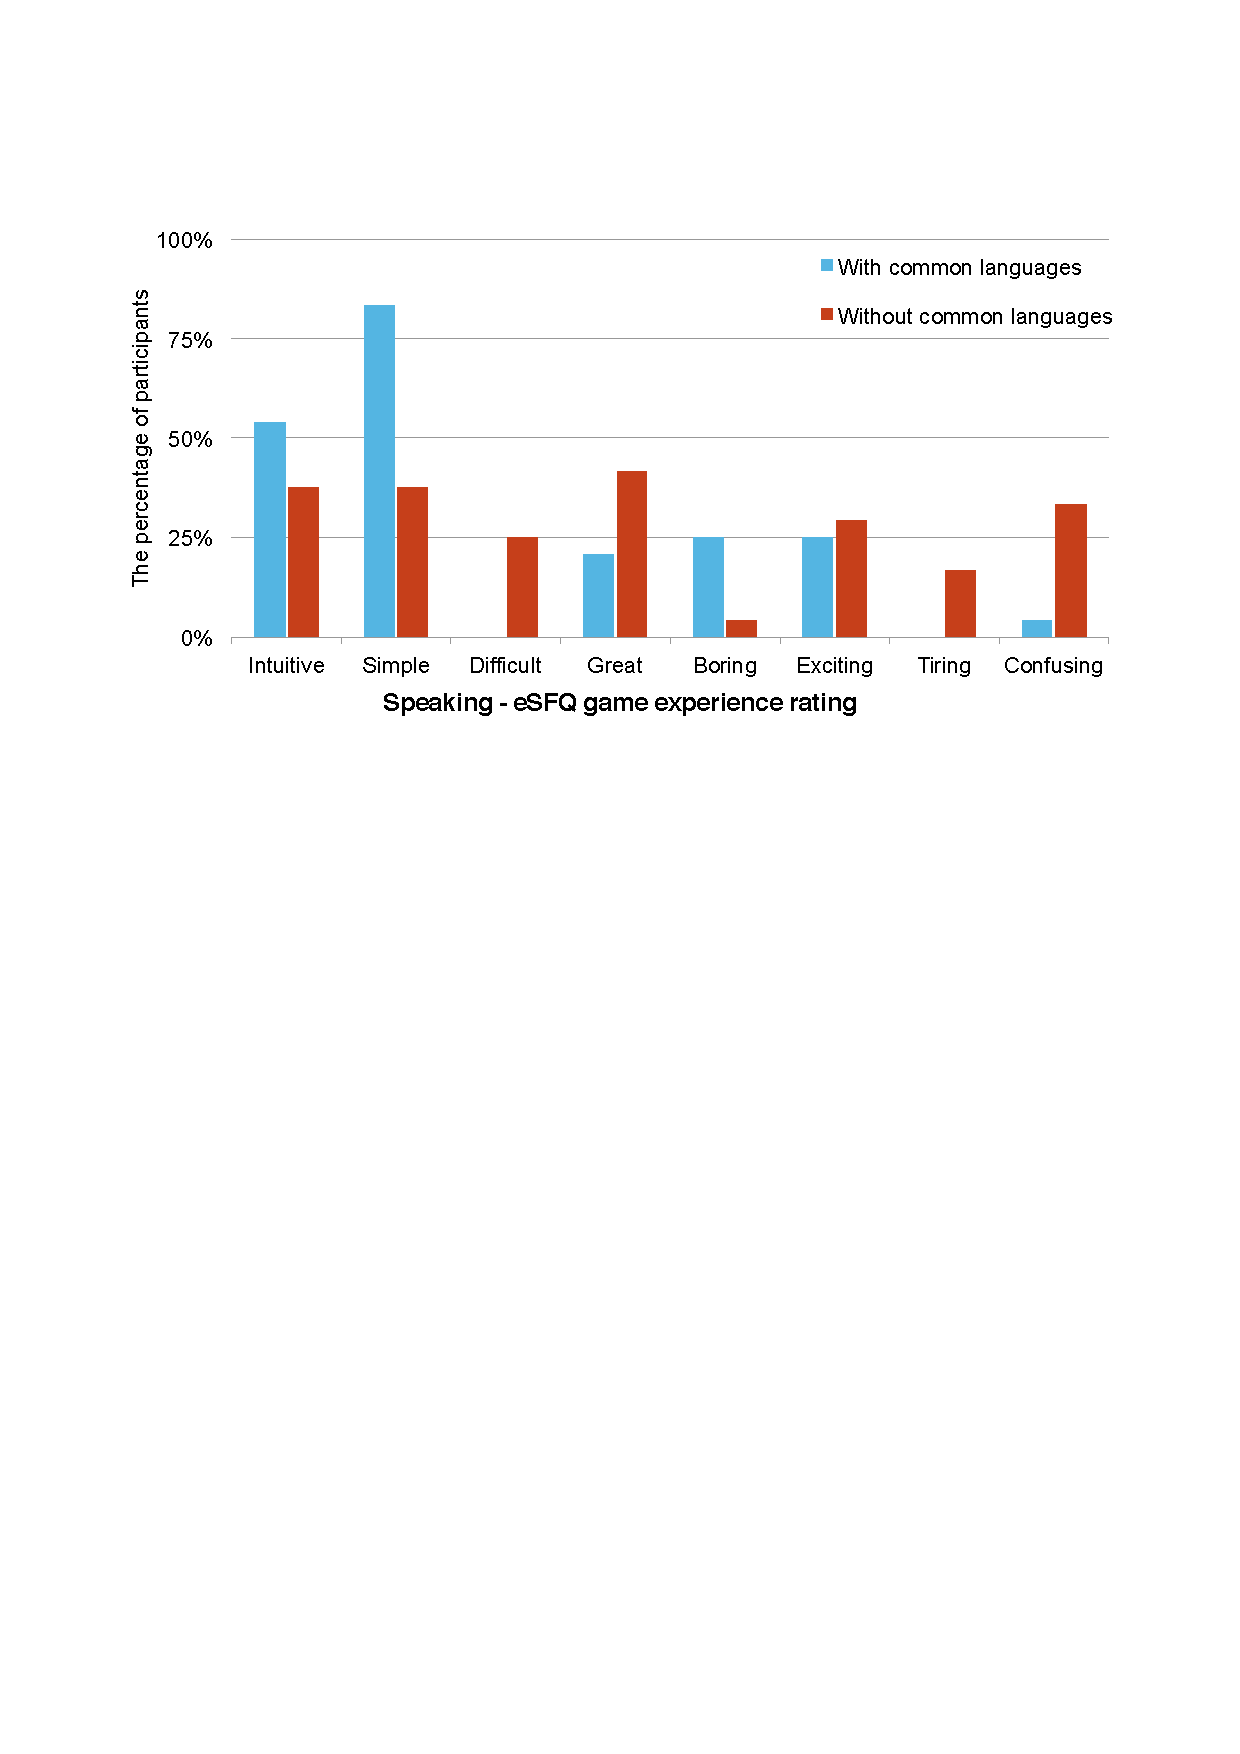
\includegraphics[width=1.0\columnwidth]{Figures/US_Consistent_Speaking.pdf}
\caption{Index patterns of eSFQ game experience rating for speaking}
\label{fig:US_Consistent_Speaking}
\end{figure}

\begin{figure}[!h]
\centering
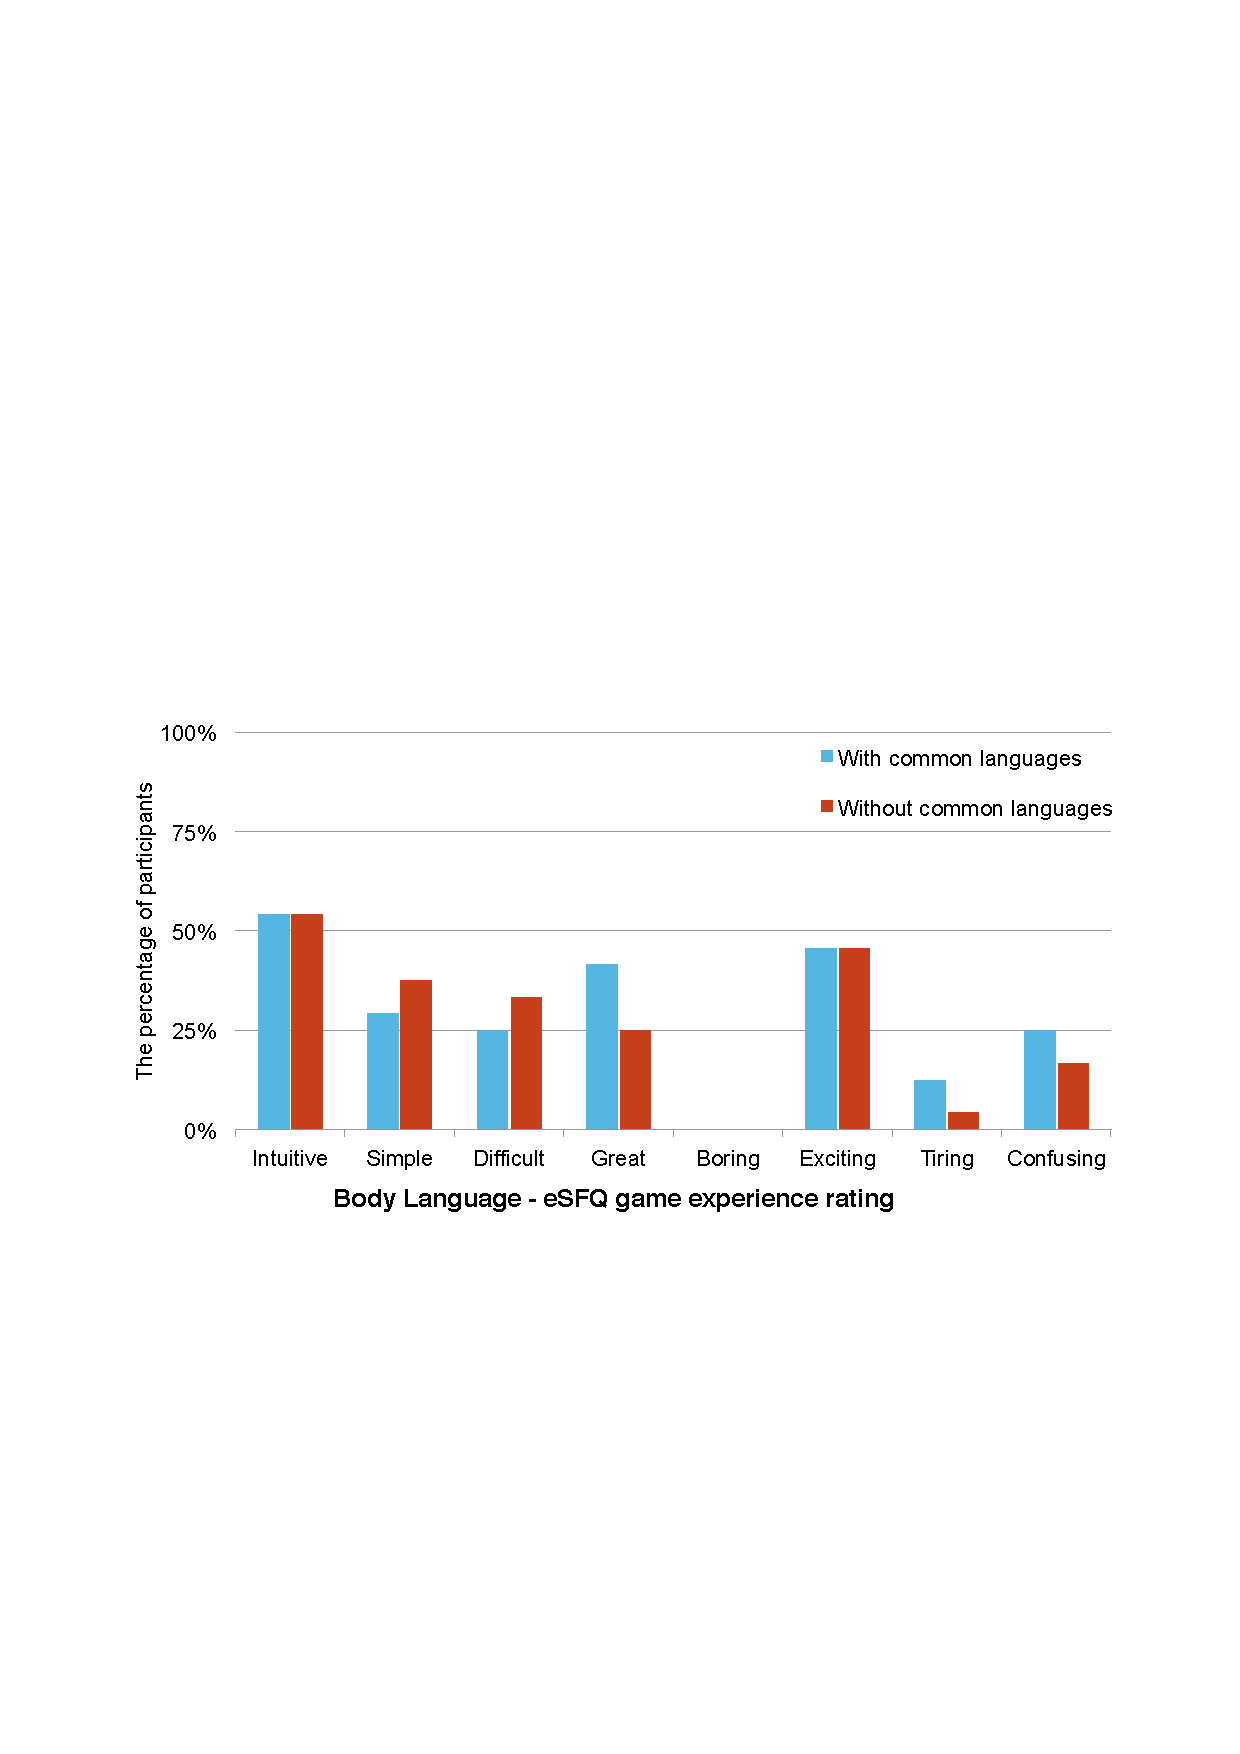
\includegraphics[width=1.0\columnwidth]{Figures/US_Consistent_Bodylanguage.pdf}
\caption{Index patterns of eSFQ game experience rating for body language}
\label{fig:US_Consistent_Bodylanguage}
\end{figure}

%, the difference in rating by players with and without common languages was much more similar when communicating only via body language. The  

%and Table~\ref{tab:Consistency}, we can observe that, with traditional setting (speaking), the eSFQ index patterns are inconsistent(the average difference is 22.40\%). In other words, it's a different game experience. However, with our body language communication manner design, the eSFQ 
%and CPMs 

%index patterns are similar (the average difference is 6.25\%). It implies cooperative game has more consistent game experience with body language communication.


% \begin{figure}[!h]
% \centering
% \includegraphics[width=0.5\columnwidth]{Figures/US_Consistent2.png}
% \caption{index pattern of CPMs}
% \label{fig:US_Consistent2}
% \end{figure}

\subsection{Communication Patterns}
We summarize the communication patterns we observed when participants were communicated by: speaking, body language, and both speaking and body language.

\subsubsection{Speaking}
For participants with common languages, communicating by speaking was straight-forward. For participants without common languages, although there were language barriers, they still found ways communicate with each other by tones, short words, and sounds.

\begin{enumerate}
   \item Simple words: participants spoke simple words and short sentences. For example, Japanese speakers would say ``hai (yes)'', ``ie (no)'', ``koko (here)'', and ``soko (there)''.
   
     \item Repeating continuously: participants often repeated the same simple words until the other player performed the corresponding action. For example, Japanese speakers would repeat ``kuru (come)'' until the the other player come. The player receiving the words would try different actions until the repeating stops. 
  
     \item Emphasized tones: participants frequently used different tones to express doing things right vs doing things wrong. They often used calm and longer repeating tones to express doing alright, and used urgent repeating tones to express doing things wrong. For example, Japanese speakers would say ``hai (yes)'' in a calm tone to express correct, and say ``ie (no)'' in an urgent tone to express wrong.
   
  % For example, such as ``YES'' or ``NO'', use simple words to disassemble complex instruction.

  
% \item Move more: moving avatar constantly to express some elements such as position, direction etc.
  
  \item Sound imitation: we observed participants mimicking animals' sounds to express the corresponding animals, such as roosters.
\end{enumerate}

\subsubsection{Body Language}
We observed similar body languages communication for players with and without common languages. We summarize them below:

\begin{enumerate}
  \item Divide and conquer: player who received puzzle-solving hints would perform one action at a time, then stops until the other player completes the corresponding action. For example, a player jumped in a particular place several times in order to imply that the other player should move to and jump at the corresponding position (see Figure~\ref{fig:US_F2}). This was the most frequently used communication pattern.

  \item Repeat it all: player who received the puzzle-solving hints would perform all the actions in one go before stopping for the other player to follow. For example, in one of our game stages shown in Figure~\ref{fig:US_F2}, the 3 buttons on the floor had to be stepped on one after another in a specific order. The top player would perform the sequence all at once for the bottom player to repeat. 
                                   
  \item Pictogram: players would use their own body to express and mimic the hints. As shown in Figure~\ref{fig:US_F3}, one participant wanted to express the letter ``N'' to the other player. Her solution was using her body to perform a pictogram.
\end{enumerate}

\begin{figure}[!t]
\centering
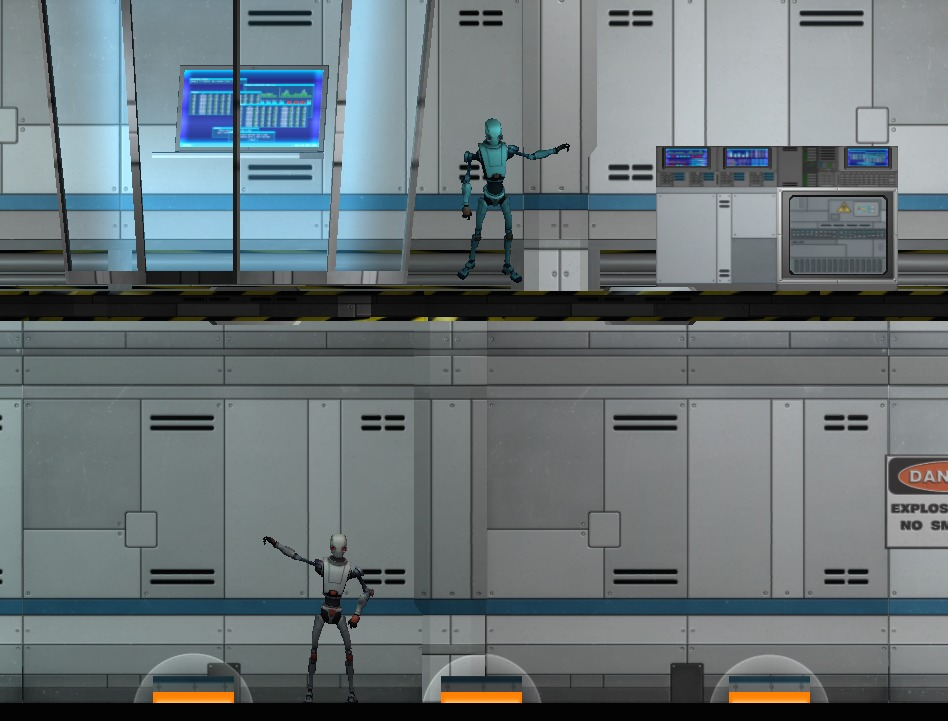
\includegraphics[width=0.7\columnwidth]{Figures/US_F2.jpg}
\caption{A sequence puzzle from Mute Robot. The top player knows the correct sequence and is showing the bottom player to move to and jump on the center yellow button among the three buttons.}
\label{fig:US_F2}
\end{figure}

\begin{figure}[!t]
\centering
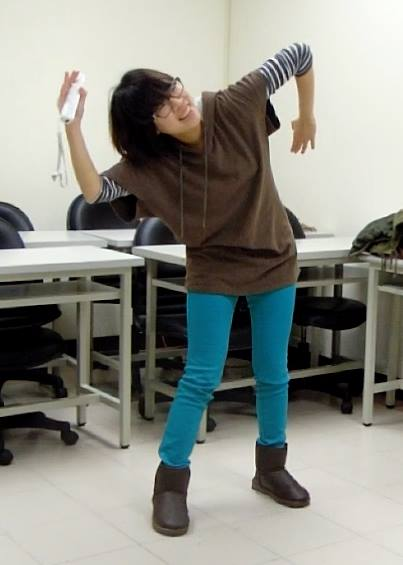
\includegraphics[width=0.4\columnwidth]{Figures/US_F3.jpg}
\caption{A participant performing a pictogram (the letter ``N'') using body language.}
\label{fig:US_F3}
\end{figure}


\subsubsection{Both Speaking and Body Language}
When both speaking and body language were available for communication, the players without common languages primarily used body language communication, and used tones and word to facilitate, such as when confirming a correct action. Players with common languages primarily communicated by speaking, and used body language to facilitate. 


%
%The difference between groups was the proportion of communication patterns ttonehat they used.
%
%\begin{enumerate}
%  \item Mixture usage: using both speaking and body language together to transmit messages and assist illustration.
%
%  \item Choosing only one pattern from speaking or body language: users will choose the most suitable or favorite communication manner, and maybe change when special condition happened.
%\end{enumerate}


\subsection{Player Feedback}
We summarize participants' feedback below:
\begin{enumerate}
  \item Fun: players reported that adding body language to cooperative gameplay enhanced gaming experience and enjoyment. For example, one participant reported ``body language is intuitive, without restriction, really funny and becoming an innovative way for a cooperative game.'' (P34), and another reported
	``For cooperative games, it's nice to be possible to be mis-understood, add something new to the gameplay'' (P18).

%“body language is intuitive, without restriction, really funny and innovative way for cooperative game.”
%“For cooperative game , it's nice to possible to be misunderstand,it's add something to the game is better.” 


  \item Voice: players found that voice improved the gaming experience compared to only using body language. For example, one participant reported that ``it is too silent when playing with only body language, I feel less lonely with voice.'' (P5) and another said ``it is more fun to hear the other player in addition to body language'' (P19).

%,It is funny to hear the other player as well
%只用肢體語言玩遊戲太過安靜了
%跟陌生人直接講話會感到尷尬,使用肢體語言則沒有這種困擾

  \item Interactivity: players reported that having body language enriched the game's interactivity. For example, players reported ``Body language provides more challenges and feels like really playing with my partner.''(P37), ``I feel embarrassed talking to a stranger, but using body language is not.'' (P23), and another player reported ``It's great to move your body, and it's more interactive'' (P11). 

%比較有挑戰性,可以互動,真的在跟他玩
%body, 跟平常不一樣的互動體驗,運動肢體的感覺很快樂 , 比較有互動的感覺


  \item Preferred communication methods: one player reported ``Using body language to communicate is more challenging, and more rewarding.''(P37), yet another player reported preference for having both speaking and body language because ``you can use whatever you prefer to communication to your partner to convey your meaning.''(P48). 

%body language比較有挑戰性,使用肢體讓別人瞭解會比較有成就感
%Different manner of communicating, you can use whatever you want to make your partner to get your meaning


\end{enumerate}

\subsection{Consistency in Game Experience}
% As we can see in Figure~\ref{fig:US_Consistent} and Table~\ref{tab:Consistency}, we can observe that, with traditional setting (speaking), the eSFQ and CPMs index patterns are inconsistent(the average difference is 22.40\% and 2.90 times). In other words, it's a different game expereience. However, with our body language communication manner design, the eSFQ and CPMs index patterns are similar(the average difference is 6.25\% and 1.00 time). It implies cooperative game has more consistent game experience with body language communication.

\begin{figure}[!h]
\centering
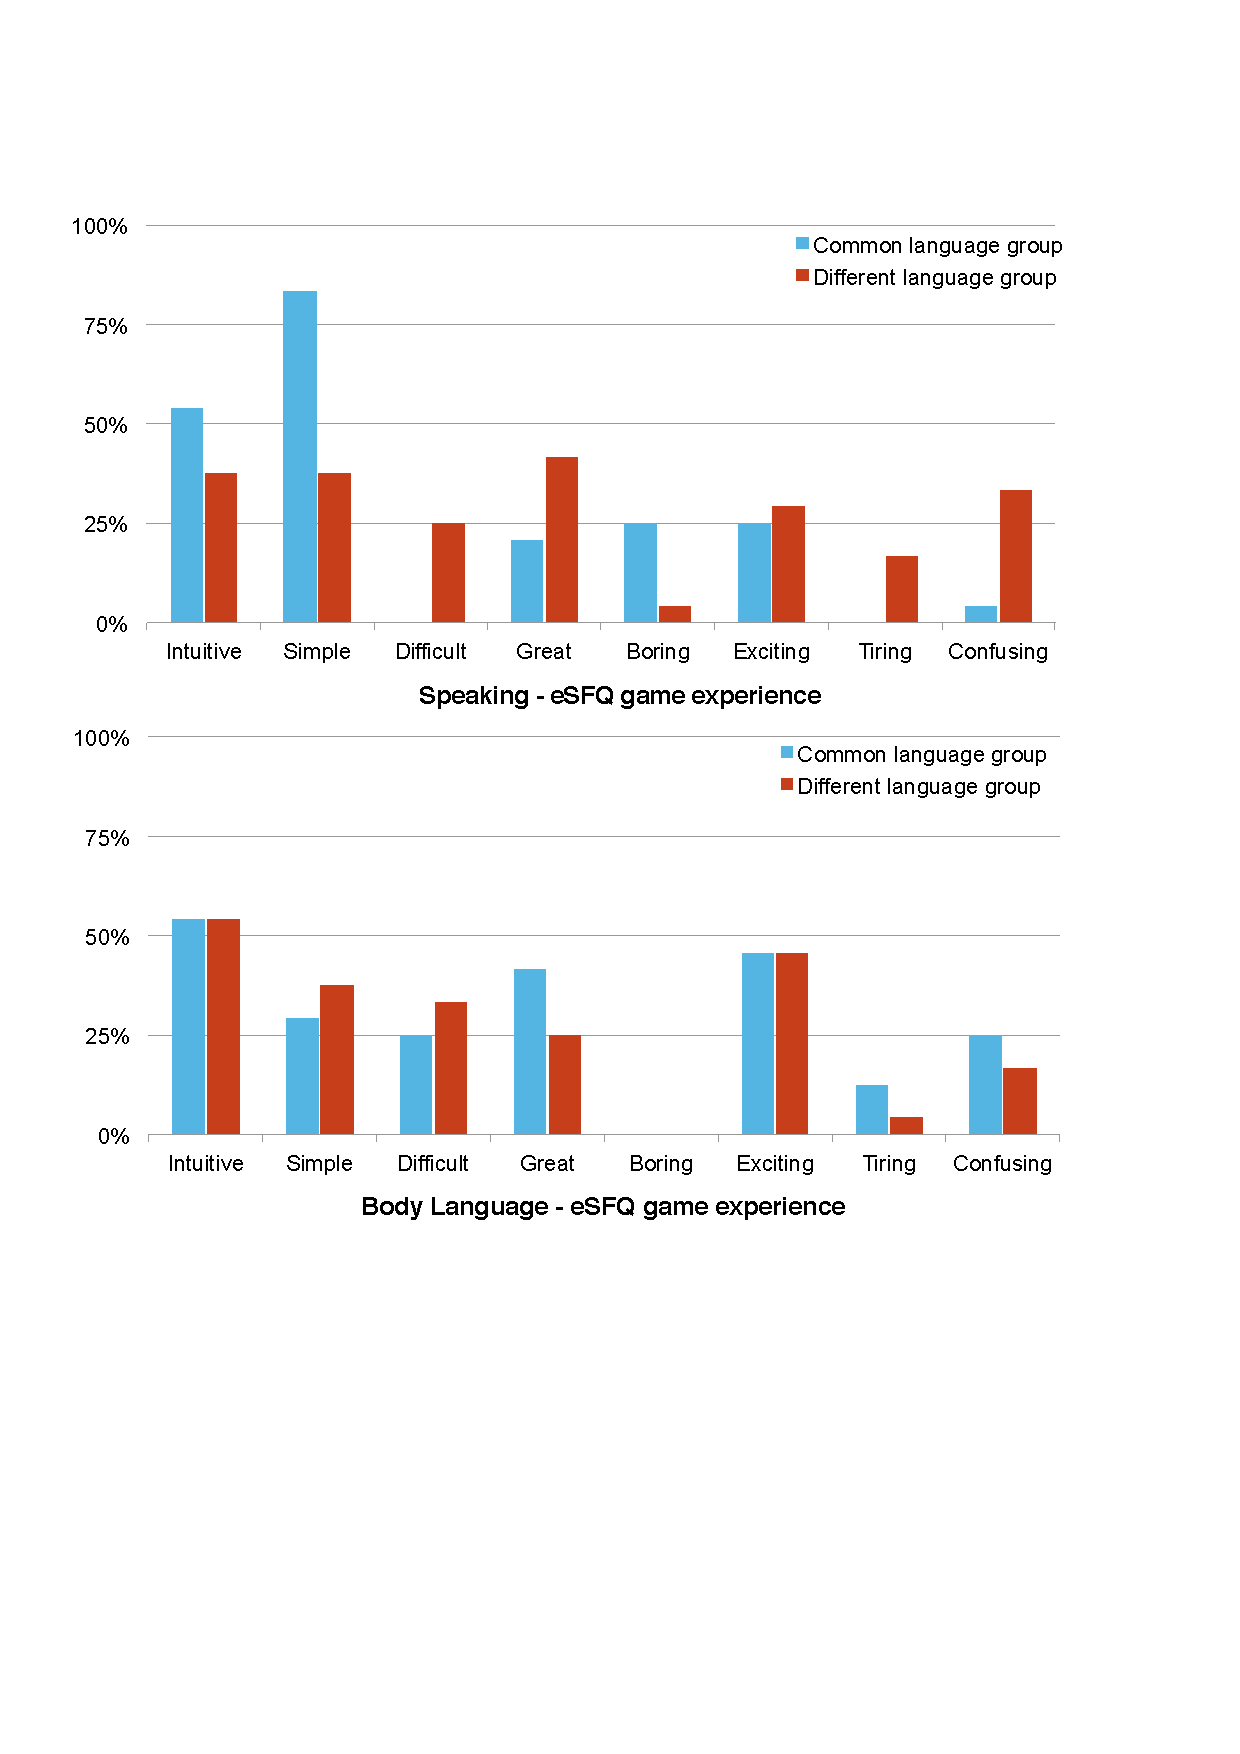
\includegraphics[width=1.0\columnwidth]{Figures/US_Consistent.pdf}
\caption{Index patterns of eSFQ game experience rating}
\label{fig:US_Consistent}
\end{figure}
%
%\begin{table}[!h]
%\renewcommand\arraystretch{1.5}
%  \centering
%  \begin{tabular}{
%  !{\vrule width2pt}c
%  !{\vrule width2pt}c
%  % !{\vrule width2pt}c
%  !{\vrule width2pt}}
%    \Xhline{2pt}
%    \multicolumn{1}
%    {!{\vrule width2pt}c!{\vrule width2pt}}
%    {\tabhead{}} &
%    \multicolumn{1}
%    {c!{\vrule width2pt}}
%    {\centering\tabhead{average difference of eSFQ game experience}} \\
%    % \multicolumn{1}
%    % {c!{\vrule width2pt}}
%    % {\centering\tabhead{CPMs (count)}} \\
%    \Xhline{2pt}
%    Speaking & 22.40\%\\
%    \Xhline{2pt}
%    Body Language & 6.25\%\\
%    \Xhline{2pt}
%  \end{tabular}
%  \caption{Average Difference between players \textit{with} and \textit{without} common languages from Figure~\ref{fig:US_Consistent}}
%  \label{tab:Consistency}
%\end{table}

Figure~\ref{fig:US_Consistent} shows the eSFQ game experience ratings for players with and without common languages, when communicating only by speaking. The experience ratings by the two player groups varied significantly. However, as shown in Figure~\ref{fig:US_Consistent}, the ratings between players with and without common languages was much more consistent when communicating via only body language. The average absolute difference in ratings was 22.4\% across the 8 indexes when communicating by speaking, compared to 6.25\% by body language only.

%, the difference in rating by players with and without common languages was much more similar when communicating only via body language. The  

%and Table~\ref{tab:Consistency}, we can observe that, with traditional setting (speaking), the eSFQ index patterns are inconsistent(the average difference is 22.40\%). In other words, it's a different game experience. However, with our body language communication manner design, the eSFQ 
%and CPMs 

%index patterns are similar (the average difference is 6.25\%). It implies cooperative game has more consistent game experience with body language communication.


% \begin{figure}[!h]
% \centering
% \includegraphics[width=0.5\columnwidth]{Figures/US_Consistent2.png}
% \caption{index pattern of CPMs}
% \label{fig:US_Consistent2}
% \end{figure}



\subsection{System Limitation}
%write more
Our prototype currently uses version 1 of the Kinect sensors, which can only track the major skeletal movements (head, torso, arms, and legs). It could not track more subtle expression such as eyes and facial expression, that are also important for non-verbal communication. In addition, it can not track finger and hand movement. As one participant reported: ``The avatar can't fully express what people can express, like emotional reaction.''

We plan to use improved sensors, such as the Kinect v2 sensors, that can capture players' more subtle movements such as hands and fingers. Furthermore, we plan to use computer vision techniques to capture and relay players' facial expressions.

%	Based on the physical devices, we would have some system limitation which may influenced little players experience. For example, we use Kinect(v1) to capture players movement, but according to the limitation of sensitivity and finite accuracy, Kinect can't capture players subtle movement, such as finger movement and facial expression. One of our user reported that ``Kinect can't provide enough sensitivity, so it can't capture subtle movements, and it has a delay.'', and 
%	another user reported ``The avatar can't fully express the things that people can express, like the emotional reaction.''.


	% Our system limitation was depend on the physical devices, like the limitation of sensitivity and accuracy of Kinect. Kinect can't capture player's subtle movements, such as finger movements and facial expression. One user reported that ``Kinect can't provide enough sensitivity, so it can't capture subtle movements, and it has a delay.'' and another user reported ``The avatar can't fully express the things that people can express, like the emotional reaction.''.

% \subsection{Summary}
% After our user experiment, user interview, questionnaire review and analysis, we integrated some main points for adding body language for cooperative gameplay experience. When we are playing games, we couldn't understand another player's meaning if there was language obstruction between both of you. In order to relief this perplexity, users needed to guess what each other wanted to express. This means they need one more language transformation until they build up their tacit agreement. We called this ``Guess Process''. During this process, users will have more interaction with each other such as helping each other. Most of these interactions were interesting to users. And 
% game enjoyment becomes higher than before.

% \subsubsection{speaking}
% For ``Speaking'', it resulted in enormous different gameplay experience between common language and different language groups. In different language group, player couldn't realize what another player wanted to express and thus they could just guess about another player's meaning under ``Guess Process''. Guess process not only made the enhancement of game difficulty but it also increased game amusement. 


% \subsubsection{body language}
% About ``Body language'', Both common language and different language groups would occur ``Guess Process'', which increased gameplay enjoyment for both group. Body language provided great cooperative experience.
% In this section, gameplay difficulty was similar to all players, which meant it had difficulty normalization and applied identically gameplay experience.

% \subsubsection{using speaking and body lanuguage together}
% About section of ``Both'', was the condition that adds the ``Body language'' element on the basis of ``Speaking''. Although language obstacle had an impact on gameplay experience no matter on common language groups or different language groups, the enjoyment of playing the game was better than traditional manner (speaking). 

% \subsection{Summary}
% After our user experiment, user interview, questionnaire review and analysis, we integrated some main points for adding body language for cooperative gameplay experience. When we are playing games, we couldn't understand another player's meaning if there was language obstruction between both of you. In order to relief this perplexity, users needed to guess what each other wanted to express. This means they need one more language transformation until they build up their tacit agreement. We called this ``Guess Process''. During this process, users will have more interaction with each other such as helping each other. Most of these interactions were interesting to users. And 
% % it also increased game difficulty indirectly which 
% game enjoyment becomes higher than before.

% \subsubsection{speaking}
% % Now we concluded each section respectively. 
% For ``Speaking'', it resulted in enormous different gameplay experience between common language and different language groups. In different language group, player couldn't realize what another player wanted to express and thus they could just guess about another player's meaning under ``Guess Process''. Guess process not only made the enhancement of game difficulty but it also increased game amusement. 
% % However cooperative feeling and curiosity won't increase. 

% \subsubsection{body language}
% % In addition, 
% About ``Body language'', Both common language and different language groups would occur ``Guess Process'', which increased gameplay enjoyment for both group. Body language provided great cooperative experience.
% % and enhanced players' curiosity significantly to the game. 
% In this section, gameplay difficulty was similar to all players, which meant it had difficulty normalization and applied identically gameplay experience.

% \subsubsection{using speaking and body lanuguage together}
% % Last but not least, 
% About section of ``Both'', was the condition that adds the ``Body language'' element on the basis of ``Speaking''. Although language obstacle had an impact on gameplay experience no matter on common language groups or different language groups, the enjoyment of playing the game was better than traditional manner (speaking). 
% Cooperative feeling and curiosity also increased obviously. Even more interesting is that under this section, different language group are the easiest and also the most interesting manner to communicate. For this result, we thought it was because the cooperative experience had greater influence on gameplay enjoyment than the difficulty.





\section{Conclusion}

% 我們Propose a Game Design for Body language.在此遊戲設計下,透過使用者實驗的資料分析,證明了加入肢體語言會使得遊戲的體驗上升,強烈的互動感會使玩家更沈浸于遊戲,並加強夥伴間合作的感覺,而且Body language can normalize game difficulty.使不論語言通或不通的玩家都能有一致的遊戲體驗,並提供語言不通的玩家彼此能交流的一種溝通方式,由於肢體語言是十分自然的交流方式,因此十分適合在遊戲裡使用。We hope to inspire more exploration of using body language in game designs,並將遊戲的樂趣帶給更多人。

We propose a game design pattern for body language. Under this game design, 



% \section{Unimportant}

% \begin{figure}[!h]
% \centering
% 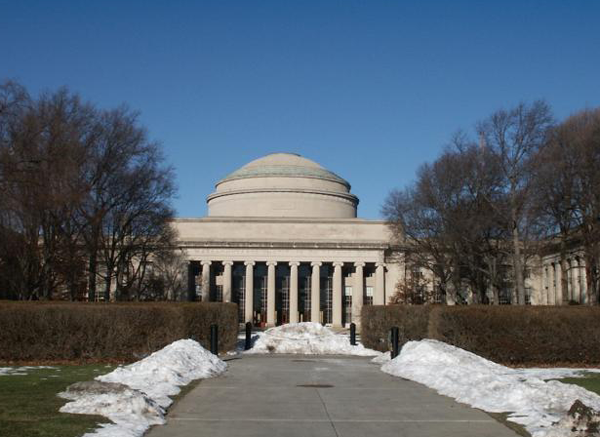
\includegraphics[width=0.9\columnwidth]{Figure1}
% \caption{With Caption Below, be sure to have a good resolution image
%   (see item D within the preparation instructions).}
% \label{fig:figure1}
% \end{figure}

% \textit{Proc. Interact 2003}). 
% \texttt{References} style
%  ``[Robertson, personal communication]''

% \begin{table}
%   \centering
%   \begin{tabular}{|c|c|c|}
%     \hline
%     \tabhead{Objects} &
%     \multicolumn{1}{|p{0.3\columnwidth}|}{\centering\tabhead{Caption --- pre-2002}} &
%     \multicolumn{1}{|p{0.4\columnwidth}|}{\centering\tabhead{Caption --- 2003 and afterwards}} \\
%     \hline
%     Tables & Above & Below \\
%     \hline
%     Figures & Below & Below \\
%     \hline
%   \end{tabular}
%   \caption{Table captions should be placed below the table.}
%   \label{tab:table1}
% \end{table}


% \section{Figures/Captions}

% (see Figure~\ref{fig:figure1}). 
% ``Table~\ref{tab:table1}'' or ``Figure~\ref{fig:figure2}''), 

% \begin{itemize}
% \item Write in a straightforward style.
% \end{itemize}

% \begin{enumerate}
% 	\item Add alternative text to all figures
% 	\item Mark table headings
% \end{enumerate}



% Balancing columns in a ref list is a bit of a pain because you
% either use a hack like flushend or balance, or manually insert
% a column break.  http://www.tex.ac.uk/cgi-bin/texfaq2html?label=balance
% multicols doesn't work because we're already in two-column mode,
% and flushend isn't awesome, so I choose balance.  See this
% for more info: http://cs.brown.edu/system/software/latex/doc/balance.pdf
%
% Note that in a perfect world balance wants to be in the first
% column of the last page.
%
% If balance doesn't work for you, you can remove that and
% hard-code a column break into the bbl file right before you
% submit:
%
% http://stackoverflow.com/questions/2149854/how-to-manually-equalize-columns-
% in-an-ieee-paper-if-using-bibtex
%
% Or, just remove \balance and give up on balancing the last page.
%
\balance

% \section{References format}
% References must be the same font size as other body text.
% REFERENCES FORMAT
% References must be the same font size as other body text.

\bibliographystyle{acm-sigchi}
\bibliography{sample}
\end{document}
